% This template is designed to operate with XeLaTeX.
%
% All elements in the Title, Abstract, and Keywords MUST be formatted as text and NOT as math.
%
%Further instructions for using this template are embedded in the document. Additionally, there are comments at the end of the file that give suggestions on writing your thesis.  
%
%In addition to the standard formatting options, the following options are defined for the VTthesis class: proposal, prelim, doublespace, draft. 

\documentclass[doublespace, nopageskip]{VTthesis} % nopageskip - Removes arbitrary blank pages.

% Using the following header instead will create a draft copy of your thesis
%\documentclass[doublespace,draft]{VTthesis}

% The lipsum package is just included to put dummy text in the document in order to demonstrate page headers and table of contents behavior. You should remove it once you begin writing your actual thesis or dissertation.
%\usepackage{lipsum}

% For the format of citations
\usepackage[sort&compress,numbers,super]{natbib}

%% Added by ZheWang-08/22/2023
%\RequirePackage[utf8]{inputenc}
\RequirePackage{chemformula}
% Script font
%\usepackage{boondox-cal}
%Tables
\usepackage{hhline}
\usepackage{multirow}
\usepackage{array}
% Equations
\def\bra#1{\langle#1 |}  
\def\ket#1{| #1 \rangle}
\def\linresp#1#2{\langle\langle#1;#2\rangle\rangle}
% Graphics
\usepackage{wrapfig}
%% End added by ZheWang


% Title of your thesis
\title{Investigation of Real-Time Coupled Cluster Methods for the Efficient Calculation of Optical Molecular Properties in the Time Domain}

% You should include 3-5 keywords, separated by commas
\keywords{Electronic structure theory, coupled cluster, numerical integration, GPUs, optical properties}

% Your name, including middle initial(s)
\author{Zhe Wang}

% Change this to your program, e.g. Physics, Civil Engineering, etc.
\program{Chemistry} 

% Change this to your degree, e.g. Master of Science, Master of Art, etc.
\degree{Doctor of Philosophy} 

% This should be your defense date:
\submitdate{September 21, 2023} 

% Committee members. Only have five readers and one chair available.
% Only use the ones you need and don't include the ones you don't need.
% You can also declare a Co-advisor. If you do, the principal and co-advisors
% will be listed as co-advisors on the title page.  Per the VT ETD standards, 
% you should not include titles or educational qualifications such as PhD or Dr.
% You should, however, include middle initials if possible.
\principaladvisor{Daniel Crawford}
\firstreader{Edward Valeev}
\secondreader{Diego Troya}
\thirdreader{Nicholas Mayhall}
%\fourthreader{Fourth Committee Member}
%\fifthreader{Fifth Committee Member}

% The dedication and acknowledgement pages are optional. Comment them out to remove them.
%\dedication{TODO}
\acknowledge{
    I would like to express my gratitude to the following individuals for guiding, supporting, and encouraging me throughout my academic journey:
    \begin{itemize}
        \item My parents, for their unconditional love, support, and for being my best friends.
        \item Mark, for brightening up my day, supporting me, and going on adventures with me.
        \item My friends for the encouragement and inspiration. I'm lucky to know you all.   
        \item Dr. Yang, for paying attention to my progress and always encouraging me to pursue my goals.
        \item Dr. Wu, for introducing me to the world of computational chemistry.
        \item Dr. Jaeger, for guiding me to become a scientist.
        \item Former and current members of the Crawford group: Roberto, Alex, Monika, Ashutosh, AJ, Kirk, Ben, Ruhee, Susana, Jose, Brendan, Josh, Sarah, and Aparna, for the motivation, collaboration, and insightful discussions.
        \item My committee members: Dr. Valeev, Dr. Mayhall, and Dr. Troya, for your expertise and feedback at every milestone.
        \item Last, but not least, Dr. Crawford, for guiding and inspiring me to be a better scientist and being the best mentor I could have asked for. 
    \end{itemize}
}

% The abstract is required.
\abstract{
Optical and spectroscopic molecular properties are key to characterizing the behavior of molecules interacting with an applied electromagnetic field of light. Response theory has been used for a long time to calculate such properties in the frequency domain. Real-time (RT) methods solve for the frequency-dependent properties in the time domain by explicitly propagating the time-dependent wave function. Various quantum chemical methods can be incorporated with the RT formalism, including Hartree-Fock, density functional theory, configurational interaction, coupled cluster, etc. Among these, coupled cluster (CC) methods provide high accuracy for systems with strong electron correlation, making RT-CC implementations intriguing. \\
All applications of CC methods face a substantial challenge due to their high-order polynomial scaling. For RT-CC methods, two aspects may be explored to improve the efficiency, the numerical techniques regarding the RT propagation and the reduced-scaling methods regarding CC itself. In this work, we start with the exploration of the hardware used for the calculations and the numerical integration methods for propagating the wave function parameters. Firstly, a GPU-enabled Python implementation has been developed by conducting the tensor contractions on GPUs utilizing PyTorch, a machine learning package, that has similar syntax as NumPy for tensor operations. A speedup of a factor of 14 is obtained for the RT-CCSD/cc-pVDZ absorption spectrum calculation of the water tetramer. Furthermore, to optimize the performance on GPUs, single-precision arithmetic is added to the implementation to achieve an additional speedup of a factor of two. Lastly, a group of integrators for solving differential equations are introduced to the RT framework, including regular explicit integrators, adaptive integrators, and a mixed-step-size approach customized for strong-field simulations. The optimal choice of the integrator depends on the requiring accuracy, stability and efficiency. \\
In addition to being highly accurate, CC methods are also systematically improvable and provide a hierarchy of accuracy. Based upon the RT-CCSD implementation, the coupled cluster singles, doubles and approximate triples (CC3) method, favorable for calculating frequency-dependent properties, is tailored to the RT framework for high excitation and approximate orbital relaxation. The calculation is tested on both CPUs and GPUs, with a significant speedup gained from GPUs for the water cluster test cases. To further expand the range of applications of our RT-CC implementation, dynamic polarizabilities, first hyperpolarizabilities, and the $G'$ tensor are calculated from induced electric and magnetic dipole moments using finite-difference methods. A discussion has also been conducted to compare RT-CC3 with RT-CCSD, and time-dependent nonorthogonal orbital-optimized coupled cluster doubles (TDNOCCD) method. Additionally, electron dynamics, including the Rabi oscillation and exited state to excited state transitions, have also been explored utilizing the well-developed RT-CC framework.
}
%\abstract{\lipsum [1-4]}

% The general audience abstract is required. There are currently no word limits.
\abstractgenaud{
Theoretical studies aim to match experiments, but more importantly, provide insights to interpret and predict experimental data. Calculating optical properties related to light-matter interactions is one of the most crucial tasks for characterizing molecular properties. In experiments, electromagnetic radiation in the form of light is applied to the system. The absorption or emission of light can be measured to identify, for example, the electronic structure of the molecule. In theoretical simulations, this applied radiation is represented by a perturbation operator that is added to the Hamiltonian in the Schr\"odinger equation. Quantum chemists are dedicated to developing methods that provide a better description of the spectroscopy. In the current work, the frequency, shape and the intensity of the radiation can all be finely-tuned, similar to experimental setups.\\
The framework for extracting optical properties from time-dependent trajectories of induced dipole moments is established for accurate and efficient simulations. To improve efficiency and make the method feasible for real-world applications, a strong understanding of light-matter interactions on a quantum level and proper utilization of computational resources are both necessary. Improvements achieved and presented in this dissertation demonstrate a powerful tool for a better understanding of the nature of the interaction between the system and the electromagnetic radiation.
}

% Creating \subsubsubsection 
\makeatletter
\newcounter{subsubsubsection}[subsubsection]
\renewcommand\thesubsubsubsection{\thesubsubsection.\arabic{subsubsubsection}}
\newcommand\subsubsubsection{\@startsection{subsubsubsection}{4}{\parindent}%
                                    {3.25ex \@plus1ex \@minus .2ex}%
                                    {-1em}%
                                    {\normalfont\normalsize\bfseries}}
\newcommand*\l@subsubsubsection{\@dottedtocline{4}{12em}{5em}}
\newcommand*{\subsubsubsectionmark}[1]{}
\makeatother

\setcounter{secnumdepth}{4}
\setcounter{tocdepth}{4}


\begin{document}

% The following lines set up the front matter of your thesis or dissertation and are required to ensure proper formatting per the VT ETD standards. 
  \frontmatter
  %\pagenumbering{⟨roman⟩}
  \maketitle
  \tableofcontents

% The list of figures and tables are now optional per the official ETD standards.  Unless you have a very good reason for removing them, you should leave these lists in the document. Comment them out to remove them.
	\listoffigures
	\listoftables
    %\printnomenclature %Creates a list of abbreviations. Comment out to remove it. 

% sample text for abbreviations:
%NLP is a field of computer science, artificial intelligence, and linguistics concerned with the interactions between computers and human (natural) languages.
 
%\nomenclature{NLP}{Natural Language Processing}
 
%$\sigma$ is the eighteenth letter of the Greek alphabet, and carries the 's' sound. In the system of Greek numerals, it has a value of 200. 
 
%\nomenclature{$\sigma$}{The total mass of angels per unit area}

% Attributions
    \chapter*{Attribution}
Chapters 3, 4 are coauthored by Prof. T. Daniel Crawford. Chapter 3 is additionally coauthored 
by Dr. Benjamin G. Peyton. 
Calculations, figures, tables and a majority of the text for these chapters were contributed by myself. Prof. Crawford served as a mentor for all projects and edited these chapters. For Chapter 3. Dr. Benjamin G. Peyton contributed to the Python packaged used, PyCC. For Chapter 4, Dr. H{\aa}kon Emil Kristiansen provided TDNOCCD polarizabilities.

% The following sets up the document for the main part of the thesis or dissertation. Do not comment out or remove this line.
	\mainmatter
	%\pagenumbering{⟨arabic⟩}
    \chapter{Introduction}  \label{intro} 
Spectroscopy is one of the most powerful tools used by scientists to understand the structure and properties of physical systems. In chemistry, spectroscopy is applied for obtaining characteristic quantities of matter and its chemical environment. An electromagnetic radiation source can be set up in the experiments, and then the impact of the radiation on the system is measured as a function of wavelength and frequency.\cite{Svanberg2023} As for the theoretical counterpart, quantum chemical methods based on the Schr\"odinger equation are developed for calculating the properties of excited states or response properties induced by the external electromagnetic field.\cite{Szabo2012, Helgaker2013} They bridge, validate and guide the experimental studies. Applications include but are not limited to: utilizing UV absorption spectra calculated with density functional theory (DFT) for the determination of Molnupiravir, a drug developed for mild COVID-19, in a more environmental friendly pharmaceutical preparation;\cite{Abdelazim2023} predicting interstellar molecules guided by a coupled cluster (CC) calculation of rotational spectra for astronomical searches;\cite{Puzzarini2023} rapid classification of tea products incorporating configuration interaction (CI) calculations with experimental X-ray photoelectron spectroscopy (XPS).\cite{Jiang2022} The development of an efficient and accurate method for calculating such properties is always highly in need, especially for higher-order properties, such as specific rotation, which are much more demanding in terms of computational resources compared to energies or dipole moments.\cite{Pecul2005, Crawford2007, Bohle2021}

For quantum chemical calculations, solving the Schr\"odinger equation is essential. However, obtaining the exact solution is only feasible for the simplest systems. The Hartree-Fock (HF)\cite{Slater1951, Szabo2012} approximation of the wave function is one of the most fundamental in computational chemistry. The essence of the Hartree-Fock approximation lies in representing the many-electron wave function as a single determinant composed of molecular orbitals, known as a Slater determinant. This single configuration state function is commonly utilized as a reference state for various higher levels of theory. Other more accurate approaches based upon HF are called post Hartree-Fock (post-HF) methods accordingly which include electron-electron correlation that is beyond the Slater determinant. For example, the configuration interaction (CI) method\cite{Sherrill1999} represents the exact wave function as a linear combination of Slater determinants so that all the electron configurations can be included with a complete basis (the number of N-electron functions in the basis set is infinite). Although full CI can give the exact solution of the N-electron problem formally, it is often extremely expensive whereas truncated CI is not size-consistent or size-extensive leading to difficulties in studying larger systems. Another important approximation for the correlation energy is coupled cluster (CC) theory.\cite{Crawford2000} Different from CI, the coupled cluster operator applies to the reference wave function in an exponential form. This unique exponential \textit{ansatz} gives rise to the most important characteristics of coupled cluster, size-consistency and size-extensivity. CC methods are systematically improvable and in practice, they are often used in truncated form. Coupled cluster singles and doubles with a perturbed triples correction (CCSD(T))\cite{Purvis1982} is referred to the gold standard. Other truncated CC methods include CCD, CCSD, CC2,\cite{Christiansen1995} CC3,\cite{Koch1997} CCSDT, etc. In this work, CC serves the role of the wave function approximation binding with the approaches targeting response properties. Since CC methods are the substantial part of the foundation and the objectives in this work, the basis and working equations that are used in Chapters 3 and 4 will be presented in Chapter 2. 

For the response properties specifically, response theory and real-time methods are two prominent approaches. Molecular properties induced by frequency-dependent external fields must naturally be calculated with a time-dependent approach. In 1928, Rosenfeld first published time-dependent perturbation methods and defined two optical activity tensors (also known as Rosenfeld tensors) that are related to the polarizability and the specific rotation respectively, laying the foundations of subsequent studies.\cite{Rosenfeld1929} To avoid the summation over all the excited states involved in the formula of Rosenfeld tensors, linear response theory (LR)\cite{Olsen1985, Sekino1984} becomes a more practical and conventional approach with the excited states replaced by the response of the ground state. The frequency-dependent response functions for the optical activity tensors are derived starting from a time-dependent perturbed Hamiltonian. Response theory agrees with the experimental data very well, especially for spectroscopic properties.\cite{Kobayashi1994, Roos1996, Coriani2012} Its root in perturbation theory, however, limits its applications to strong external fields. In Chapter 4, LR, particularly LR-CC results are used as the reference values in the examination of the accuracy of the proposed novel approaches where weak interactions between the molecules and the fields are involved. The fundamentals will be included in Chapter 2. 

Real-time methods, on the other hand, are non-perturbative approaches that can cope with strong external fields beyond perturbation theory.\cite{Goings2018, Li2020} With an explicit time-dependence, properties are calculated in the time-domain by propagating wave function parameters based on the time-dependent Schr\"odinger equation (TDSE). The properties can further be transformed into the full frequency-domain by means of, for example, Fourier transform (FT) without a designated narrow frequency range. Other advantages including the natural connection to the experiments, the potential of combining advanced techniques in other fields such as laser spectroscopy and numerical integration are also key drivers of the development of real-time methods. As mentioned earlier, this work will focus on implementations within the CC approximation. For real-time coupled cluster (RT-CC) methods, the challenge lies in two aspects: (1) The long propagation time for high-resolution spectra and the small step size for the adequate numerical stability of the simulation; (2) The balance between better accuracy with higher levels of theory and the high computational cost stemming from the polynomial scaling of CC methods. As a guide of general RT-CC simulations, the derivation of the differential equations of the coupled cluster amplitudes and the consideration of the external field and resulting properties are included in Chapter 2. 

Studies that seek for strategies to accelerate the simulations are shown in Chapter 3. Three perspectives are given: investigating the capability of the single-precision arithmetic compared to the conventional double-precision in quantum chemistry for the properties of interest; migrating the calculation from CPUs to GPUs to speed up the tensor contraction which is the major component of the working equations and the most expensive part of the calculation; and adopting and tailoring adaptive numerical integrators for RT-CC methods in order to lower the computational cost and improve the numerical stability particularly considering the high-intensity external fields. Chapter 4 presents the derivation and applications of real-time approximate coupled cluster singles, doubles and triples (RT-CC3) model with the singles amplitudes treated as zeroth-order and performing a function of  approximate orbital relaxation parameters. In addition to the absorption spectrum, polarizability, first hyperpolarizability and $G'$ tensor that is related to the optical rotation are also extracted from the real-time simulation with finite-difference methods.\cite{Ding2013} Results are compared to other RT-CC methods. Notably, a comparison with real-time (RT) time-dependent nonorthogonal orbital-optimized coupled cluster doubles (TDNOCCD)\cite{Krylov2000, Pedersen2001, Kristiansen2020} is carried out to explore more information about the mechanism and importance of orbital relaxation in real-time methods. A summary and conclusion section is given in Chapter 5. 
    \chapter{Theoretical Background}  \label{theory} 
\section{Approximations of the Many-Electron Wave Function}\label{approx-wfn}
A primary goal of quantum chemists is to identify suitable approximations for the many-electron wave function under specific circumstances. As frequently observed in quantum chemical investigations, key approximations are employed to account for various factors, such as neglecting relativistic effects\cite{Pitzer1979} that become significant for systems containing very heavy atoms and applying the Born-Oppenheimer approximation\cite{Born1927} that treats the wave functions of nuclei and electrons separately due to the substantial difference in mass and velocity between nuclei and electrons. These approximations lead to the formulation of the non-relativistic time-dependent electronic Schr\"odinger equation\cite{Schrodinger1982} (TDSE) in atomic units,
\begin{equation}
\hat{H}\ket{\Psi(\mathbf{r}, t; \mathbf{R})} = i\frac{d}{dt}\ket{\Psi(\mathbf{r}, t; \mathbf{R})},
\end{equation}
where the wave function depends on electronic coordinates and time explicitly and nuclear coordinates implicitly. Furthermore, for any stationary states without the consideration of the time-dependency, we can use a simpler form, the time-independent Schr\"odinger equation (TISE), 
\begin{equation}
\hat{H}\ket{\Psi(\mathbf{r}; \mathbf{R})} = E\ket{\Psi(\mathbf{r}; \mathbf{R})},
\end{equation}
which is an eigenvalue problem where the wave function and the energy of the corresponding state is the eigenvector and eigenvalue of the Hamiltonian, respectively.  

To completely describe an electron, the form of the wave function must also incorporate principles associated with spin and the Pauli exclusion principle.\cite{Pauli1925} One commonly used representation is the Slater determinant in the Hartree-Fock (HF) approximation,\cite{Slater1951, Szabo2012}
\begin{equation}
\Psi(\mathbf{x_{1}}, \mathbf{x_{2}}, ..., \mathbf{x_{N}})=(N!)^{-\frac{1}{2}}
\begin{vmatrix}
\chi_{1}(\mathbf{x_{1}}) & \chi_{2}(\mathbf{x_{1}}) & \cdots & \chi_{N}(\mathbf{x_{1}}) \\
\chi_{1}(\mathbf{x_{2}}) & \chi_{2}(\mathbf{x_{2}}) & \cdots & \chi_{N}(\mathbf{x_{2}}) \\
\vdots & \vdots & \ddots & \vdots \\
\chi_{1}(\mathbf{x_{N}}) & \chi_{2}(\mathbf{x_{N}}) & \cdots & \chi_{N}(\mathbf{x_{N}})
\end{vmatrix}, 
\end{equation}
where the orbital $\chi(\mathbf{x})=\phi(\mathbf{r})\alpha(\omega) \ or \ \phi(\mathbf{r})\beta(\omega)$ includes both spatial and spin coordinates.As a result, a wave function described by a single Slater determinant has $N$ electrons occupying $N$ spin orbitals and adheres to the Pauli exclusion principle/antisymmetry principle. It also accounts for the exchange correlation between two electrons with parallel spins, while the motions of electrons with opposite spins remain uncorrelated. Thus, HF methods are often referred to as ``uncorrelated" methods. Despite missing some of the exchange correlation terms, the HF approximation serves as the foundation for many other more accurate ``correlated" methods. For instance, the wave function can be represented as a combination of the HF ground state wave function $\ket{\Psi_{0}}$ and other determinants built upon $\ket{\Psi_{0}}$ as the reference state. Such methods are also known as post-HF methods.

\section{Coupled Cluster Methods}\label{cc}
Coupled cluster (CC) theory\cite{Crawford2000} is one of the post-HF methods that considers the correlated motions of any pair of electrons. Compared to HF, the correlated wave function consists not only of occupied orbitals as in the Slater determinant, but also of unoccupied/virtual orbitals that are part of the basis set but possess higher energy. By substituting occupied orbitals with virtual ones, excited/substituted determinants are constructed to enhance electron correlation. A linear combination of the HF ground state and these excited determinants is employed to provide a more accurate approximation of the wave function. In contrast to other correlated methods, CC methods use an exponential \textit{Ansatz} to specifically incorporate excited determinants:
\begin{equation}
\ket{\Psi_{\rm CC}} = e^{\hat{T}} \ket{0},
\label{eq:cc-wfn}
\end{equation}
and TISE becomes
\begin{equation}
\hat{H}e^{\hat{T}} \ket{0} = E_{CC}e^{\hat{T}} \ket{0},
\end{equation}
where the reference state, $\ket{0}$, is often the HF ground state. The excitation operator $\hat{T}$ in Eq.~(\ref{eq:cc-wfn}) can be expanded and represented with a convenient mathematical technique, second quantization:\cite{Dirac1927}   
\begin{equation}
\hat{T} = \sum_{n=1}^{N}\hat{T}_{n},
\end{equation}
with the nth-orbital cluster operator as
\begin{equation}
\hat{T}_{n} = (\frac{1}{n!})^{2}\sum_{ij...ab...}t_{ij...}^{ab...}a_{a}^{+}a_{b}^{+}...a_{j}a_{i},
\end{equation}
where $i, j, ...$ denotes occupied orbitals, $a, b, ...$ denotes virtual orbitals, and $t_{ij...}^{ab...}$ are excitation amplitudes corresponding to the n-tuply excited determinant, $\ket{\Psi_{ij...}^{ab...}}$. $a_{p}^{+}$ and $a_{p}$ are the creator and the annihilator, respectively, for any orbital $p$ in the second quantization. An exact description of the wave function can be obtained by including all possible excited determinants. However, in practice, truncated CC methods are usually employed due to their polynomial scaling and the limitation of computational resources. For example, the coupled cluster singles and doubles (CCSD) method includes only single- and double-excitation terms with $\hat{T}=\hat{T}_{1}+\hat{T}_{2}$. Its scaling is proportional to $N^{6}$, which is the order of the most computationally expensive contraction in CCSD equations. Similarly, the gold standard in quantum chemistry, CCSD(T),\cite{Raghavachari1989} scales as $N^{7}$, while CCSDT,\cite{Noga1987} which includes all triple excitations, scales as $N^{8}$.

The CC energy, $E_{CC}$, and $\hat{T}$ amplitudes can be solved by left-projecting the reference state $\ket{0}$ and the excited determinants $\ket{\Psi_{ij...}^{ab...}}$ to the Schr\"odinger equation, respectively:
\begin{equation}
\bra{0}e^{-\hat{T}}\hat{H}e^{\hat{T}} \ket{0} = E_{CC}\bra{0}e^{-\hat{T}}e^{\hat{T}} \ket{0} = E_{CC},
\label{eq:cc-energy}
\end{equation}
\begin{equation}
\bra{\Psi_{ij...}^{ab...}}e^{-\hat{T}}\hat{H}e^{\hat{T}} \ket{0} = E_{CC}\bra{\Psi_{ij...}^{ab...}}e^{-\hat{T}}e^{\hat{T}} \ket{0} = 0.
\label{eq:cc-amp}
\end{equation}
Noting that the similarity-transformed Hamiltonian, $e^{-\hat{T}}\hat{H}e^{\hat{T}}$, has the same eigenspectrum as $\hat{H}$ and is introduced by multiplying an inverse exponential $e^{-\hat{T}}$ in the process, so that the right-hand side of Eq.~(\ref{eq:cc-amp}) does not involve $E_{CC}$, the similarity-transformed Hamiltonian is usually denoted as $\bar{H}$. It can be calculated iteratively using the amplitudes solved via Eq.~(\ref{eq:cc-amp}). $\bar{H}$ can then be inserted into Eq.~(\ref{eq:cc-energy}) to solve for the CC energy. Another advantage of introducing $\bar{H}$ is that $e^{-\hat{T}}\hat{H}e^{\hat{T}}$ can be expanded as a linear combination of nested commutators of $\hat{H}$ with $\hat{T}$ using the Campbell-Baker-Hausdorff (CBH) expansion.\cite{Achilles2012} It can be naturally truncated at quadruply nested commutators:
\begin{equation}
e^{-\hat{T}}\hat{H}e^{\hat{T}} = \hat{H} + [\hat{H}, \hat{T}] + \frac{1}{2!}[[\hat{H}, \hat{T}], \hat{T}] + \frac{1}{3!}[[[\hat{H}, \hat{T}], \hat{T}], \hat{T}]
+ \frac{1}{4!}[[[[\hat{H}, \hat{T}], \hat{T}], \hat{T}], \hat{T}].
\label{eq:cc-cbh}
\end{equation}
In addition to simplifying the wave function mathematically, the unique exponential \textit{Ansatz} also guarantees the CC energy to be size-consistent and size-extensive,\cite{Sinanoglu1964, Cizek1966, Cizek1971, Crawford2000} with the reference wave function also being size-consistent and size-extensive. These characteristics are in demand, especially for larger molecules. Considering a system consisting of two non-interacting fragments, X and Y, $e^{\hat{T}}$ can be factorized as $e^{\hat{T}_{X}+\hat{T}_{Y}}=e^{\hat{T}_{X}}e^{\hat{T}_{Y}}$, leading to the wave function of the system as a product of the wave functions of its far-apart fragments. Thus, the corresponding CC energies have the relationship of $E_{CC}(XY) = E_{CC}(X) + E_{CC}(Y)$, which shows the size-consistency. Size-extensivity, on the other hand, is related to size-consistency but is more mathematically formal. Because $\hat{T}$ amplitudes have no dependency on the energy, as shown in Eq.~(\ref{eq:cc-amp}), the amplitudes are independent of the system size without being affected by the size-dependent energy. Also, as shown straightforwardly in the CBH expansion in Eq.~(\ref{eq:cc-cbh}), all the terms on the right-hand side have the Hamiltonian $\hat{H}$ connected to all cluster operators $\hat{T}$, regardless of whether $\hat{T}$ is truncated or not. These facts ensure that the CC energy scales linearly with the system size (the number of electrons), not only for full CC but also for truncated CC methods.

Although we have seen that $\bar{H}$ is convenient for the implementation of CC methods and the demonstration of important characteristics of CC, it is no longer Hermitian. Therefore, the left-hand eigenvectors and the right-hand eigenvectors are not identical and need to be solved separately. One way to resolve this is to introduce the energy Lagrangian:\cite{Beavis1990, Koch1990} 
\begin{equation}
\mathcal{L}_{CC} = E_{CC} = \bra{0}\bar{H}\ket{0} + \sum_{ij...ab...}\lambda_{ab...}^{ij...}\bra{\Psi_{ij...}^{ab...}}\bar{H}\ket{0} 
                                             = \bra{0}(1 + \hat{\Lambda})\bar{H}\ket{0},
\label{eq:cc-lag}                                          
\end{equation}
where $\lambda_{ab...}^{ij...}$ are the Lagrangian multipliers, also referred to as de-excitation amplitudes in CC equations. The left- and right-hand wave functions are thereby written as
\begin{equation}
\bra{\tilde{\Psi}_{CC}} = \bra{0}(1 + \hat{\Lambda})e^{-\hat{T}} 
\label{eq:cc-left-wfn}
\end{equation}
and
\begin{equation}
\ket{\Psi_{CC}} = e^{\hat{T}}\ket{0},
\label{eq:cc-right-wfn}
\end{equation}
respectively. The amplitude equations are then derived through variational optimization of $\mathcal{L}_{CC}$ with
\begin{equation}
\frac{\partial \mathcal{L}_{CC}}{\partial \lambda_{ab...}^{ij...}} = \bra{\Psi_{ij...}^{ab...}}\bar{H}\ket{0} = 0
\label{eq:cc-t-eqn}
\end{equation}
as the $\hat{T}$ equations, and 
\begin{equation}
\frac{\partial \mathcal{L}_{CC}}{\partial t_{ij...}^{ab...}} = \bra{0}(1 + \hat{\Lambda})[\bar{H}, \tau_{ij...}^{ab...}]\ket{0} = 0
\label{eq:cc-l-eqn}
\end{equation}
as the $\hat{\Lambda}$ equations, where $\tau_{ij...}^{ab...}$ is the second-quantized excitation operator.


Up to this point, equations for calculating CC amplitudes and the ground state energy have been presented. Other methods will be needed to obtain additional properties of interest. For instance, excited state energies can be calculated using equation-of-motion coupled cluster (EOM-CC) methods\cite{Geertsen1989, Stanton1993} by diagonalizing the similarity-transformed Hamiltonian. CC response theory\cite{Monkhorst1977, Dalgaard1983} is useful for studying frequency-dependent properties arising from the interaction between the system and external electromagnetic perturbations. Real-time coupled cluster (RT-CC) methods\cite{Schonhammer1978, Hoodbhoy1979} can also quantify properties related to the system's response to external electromagnetic fields, both within and beyond the perturbation theory framework. The following sections will discuss response theory and real-time methods in detail. 

\section{Response Theory}\label{response}
Apart from the molecular properties of the ground state, a variety of properties induced by the interaction between the system and an external electromagnetic field are also important for understanding molecular structure, electronic structure, electron dynamics, etc.\cite{English2015, Stuyver2020} The capability to calculate such properties, including spectroscopic properties, establishes a connection between theoretical studies and experimental measurements. Response theory, in particular, provides a framework to solve for the perturbation of a system by a time-dependent field as terms of a perturbative expansion with respect to the field strength.\cite{Norman2011, Helgaker2012} To derive the evolution of the wave function in the presence of a time-dependent field, we express the Hamiltonian as a sum of two terms with different perturbative orders: one being the zeroth-order time-independent term and the other being the first-order time-dependent term representing the field:
\begin{equation}
\hat{H}(t) = \hat{H}^{(0)} +  \hat{H}^{(1)}(t) = \hat{H}_{0} + \hat{V}^{t},
\label{eq:response-h}
\end{equation}
where
\begin{equation}
\hat{V}^{t} = \int_{-\infty}^{\infty} d\omega \, \hat{V}^{\omega}e^{-i\omega t},
\label{eq:response-V}
\end{equation}
obtained from the Fourier transform\cite{Bracewell1989} with $\omega$ being the frequency of the external field. And
\begin{equation}
\hat{V}^{\omega} = \epsilon_{\omega}\hat{\Omega},
\end{equation}
where $\epsilon_{\omega}$ represents the amplitude of the field, and $\hat{\Omega}$ represents the field operator. We can then expand the wave function and the expectation value of a general operator in orders of the perturbation as follows: 
\begin{equation}
\ket{\Psi(t)} = \ket{\Psi}^{(0)} +  \ket{\Psi(t)}^{(1)} +  \ket{\Psi(t)}^{(2)} + ...,
\end{equation}
where 
\begin{equation}
\ket{\Psi}^{(1)} = \int_{-\infty}^{\infty} d\omega \,  \ket{\Psi(\omega)}^{(1)}e^{-i\omega t}
\end{equation}
and
\begin{equation}
\ket{\Psi}^{(2)}  = \int_{-\infty}^{\infty} d\omega_{1} \int_{-\infty}^{\infty} d\omega_{2} \, 
                            \ket{\Psi(\omega_{1}, \omega_{2})}^{(2)}e^{-i\omega_{1} t}e^{-i\omega_{2} t}.
\end{equation}
Similarly, the expansion of the expectation value of an operator $\hat{A}$ can be written as
\begin{equation}
\langle \hat{A}\rangle(t) = \langle \hat{A}\rangle_{0} + 
                                     \int_{-\infty}^{\infty} d\omega \,  \langle\langle \hat{A};\hat{V}^{\omega}\rangle\rangle_{\omega} e^{-i\omega t} + 
                                     \int_{-\infty}^{\infty} d\omega_{1} \int_{-\infty}^{\infty} d\omega_{2} \, 
                                     \langle\langle \hat{A};\hat{V}^{\omega_{1}}, \hat{V}^{\omega_{2}} \rangle\rangle_{\omega_{1}, \omega_{2}} e^{-i\omega_{1} t}e^{-i\omega_{2} t} + ...,
\label{eq:response-exp-val}                                   
\end{equation}
from which the response functions are defined. $\langle\langle \hat{A};\hat{V}^{\omega}\rangle\rangle$ is the linear response function corresponding to the first-order perturbation due to the applied field and $\langle\langle \hat{A};\hat{V}^{\omega_{1}}, \hat{V}^{\omega_{2}} \rangle\rangle$  is the quadratic response function corresponding to the second-order perturbation. By definition, molecular response properties can be calculated using response functions at various perturbative orders. For example, in the presence of an external electric field, frequency-dependent polarizabilities are associated with the linear response function, while frequency-dependent hyperpolarizabilities are related to the quadratic response function. Additionally, transition matrix elements between the reference state and an excited state can be computed using the residue of the response function when the frequency of the field matches the energy difference between the two states. A wide range of molecular properties can be obtained by selecting different operators of interest and various types of external fields, such as electric or magnetic fields.\cite{Helgaker2012, Mukherjee1979, Olsen1985, Luo1995, Autschbach2002, Crawford2006, Bast2011}

To derive the response functions, one popular way is to utilize the time-dependent quasi-energy.\cite{Christiansen1998} Considering the exact states to start with, the wave function can be separated into a regular wave function $\ket{\tilde{\Psi}}$ and a time-dependent phase factor $F(t)$ with real values:
\begin{equation}
\ket{\Psi} = \ket{\tilde{\Psi}}e^{-iF(t)}.
\end{equation}
Inserting this form of the wave function into TDSE and then left-projecting the Schr\"odinger equation with $\ket{\tilde{\Psi}}$, we arrive at the equations for $F(t)$:
\begin{equation}
(\hat{H} - i\frac{d}{dt} - \frac{dF(t)}{dt} )\ket{\tilde{\Psi}} = 0.
\label{eq:response-quasi-SE}
\end{equation}
We define the time derivative of the phase factor as
\begin{equation}
Q(t) = \frac{dF(t)}{dt} = \bra{\tilde{\Psi}}\hat{H}-i\frac{d}{dt}\ket{\tilde{\Psi}},
\label{eq:response-quasi}
\end{equation}
where $Q(t)$ is the so-called quasi-energy. Noted that the quasi-energy becomes the ground state energy when the Hamiltonian is time-independent when $\hat{V}^{t} = 0$. 

With the form of $\hat{V}^{t}$ shown in Eq.~(\ref{eq:response-V}), a time-averaged quasi-energy\cite{Christiansen1998} over a period of the field $T=\frac{2\pi}{\omega}$ is essential to the response theory, which can be shown in Eq.~(\ref{eq:response-Q}):
\begin{equation}
\mathcal{Q} = \{Q\}_{T} = \{\bra{\tilde{\Psi}}\hat{H}-i\frac{d}{dt}\ket{\tilde{\Psi}}\}_{T},
\label{eq:response-Q}
\end{equation}
where the time-average is calculated as
\begin{equation}
\{Q\}_{T} = \frac{1}{T}\int_{0}^{1}Q(t)dt.
\end{equation}
It is also worth mentioning that $\mathcal{Q}$ does not depend on the form of $\ket{\tilde{\Psi}}$. Changing $\ket{\tilde{\Psi}}$ will not lead to any differences, which means that the derivation presented here for the exact states also applies to the approximate wave functions that will be discussed later on.

In analogous to the regular energy, the variational principle\cite{Ekeland1974} and the generalized Hellmann-Feynman theorem\cite{Hayes1965} of the quasi-energy are examined. By projecting an arbitrary variation of the regular wave function on Eq.~(\ref{eq:response-quasi-SE}): 
\begin{equation}
\bra{\delta\tilde{\Psi}} \hat{H} - i\frac{d}{dt} - Q(t) \ket{\tilde{\Psi}} = 0, 
\label{eq:response-variation}
\end{equation}
and taking a time-average of Eq.~(\ref{eq:response-variation}), the variational principle of the time-averaged quasi-energy can be derived as 
\begin{equation}
\delta\mathcal{Q} = 0.
\end{equation}
By taking the derivative of $\mathcal{Q}$ with respect to the amplitude of the field $\epsilon^{\omega}$, the Hellmann-Feynman theorem can be obtained as
\begin{equation}
\frac{d\mathcal{	Q}}{d\epsilon^{\omega}}=\{\bra{\tilde{\Psi}}\frac{d\hat{H}}{d\epsilon^{\omega}}\ket{\tilde{\Psi}}\}_{T}.
\end{equation}

Following the same procedure, we can also choose a different starting point rather than the one shown in Eq.~(\ref{eq:response-quasi}). The intermediate normalization together with the Lagrangian can be introduced to the derivation. The quasi-energy and the complex and real quasi-energy Lagrangian and the time-averaged Lagrangian in this formulation are derived and shown as
\begin{equation}
Q(t)  = Re(\bra{\Psi_{0}}\hat{H}\ket{\hat{\Psi}}),
\label{eq:response-lag-Q}
\end{equation}
\begin{equation}
L^{C}(t)  = \bra{\Psi_{0}}\hat{H}\ket{\hat{\Psi}} + \bra{\bar{\Psi}}\hat{H} - i\frac{d}{dt}\ket{\hat{\Psi}},
\label{eq:response-lag-Lc}
\end{equation}
\begin{equation}
L(t)  = Re(\bra{\Psi_{0}}\hat{H}\ket{\hat{\Psi}} + \bra{\bar{\Psi}}\hat{H} - i\frac{d}{dt}\ket{\hat{\Psi}}),
\label{eq:response-lag-L}
\end{equation}
and
\begin{equation}
\mathcal{L}  = Re(\{\bra{\Psi_{0}}\hat{H}\ket{\hat{\Psi}}\}_{T} + \{\bra{\bar{\Psi}}\hat{H} - i\frac{d}{dt}\ket{\hat{\Psi}}\}_{T}),
\label{eq:response-lag-avg-L}
\end{equation}
respectively, where $Q(t)$ remains real, and $L(t)$ is the real part of the complex $L^{C}(t)$. In Eqs.~(\ref{eq:response-lag-Q}) to~(\ref{eq:response-lag-avg-L}), the intermediate normalization $\bra{\Psi_{0}}\hat{\Psi}\rangle=1$ between a reference state $\ket{\Psi_{0}}$ and a normalized state $\ket{\hat{\Psi}}$ can be expanded in an orthonormal basis involving $\ket{\Psi_{0}}$ as
\begin{equation}
\ket{\hat{\Psi}} = \ket{\Psi_{0}} + \sum_{n}c_{n}\ket{\textbf{n}},
\label{eq:response-c}
\end{equation}
where $\bra{\bar{\Psi}}$ is defined as 
\begin{equation}
\bra{\bar{\Psi}}=\sum_{n}\bar{c}_{n}\bra{\hat{\textbf{n}}},
\label{eq:response-cbar}
\end{equation}
so that $\bra{\hat{\textbf{n}}}\hat{\Psi}\rangle=0$. The stationary condition of the quasi-energy Lagrangian is then obtained as
\begin{equation}
\bra{\hat{\textbf{n}}}\hat{H}-i\frac{d}{dt}\ket{\hat{\Psi}}=0,
\end{equation}
with $\bar{c}_{n}$ being the Lagrangian multipliers, giving us 
\begin{equation}
\bra{\bar{\Psi}}\hat{H} - i\frac{d}{dt}\ket{\hat{\Psi}} = \sum_{n}\bar{c_{n}}\bra{\hat{\textbf{n}}}\hat{H}-i\frac{d}{dt}\ket{\hat{\Psi}},
\end{equation}
as seen in the second term of Eq.~(\ref{eq:response-lag-Lc}).

The variational principle and the Hellmann-Feynman theorem are thereby become
\begin{equation}
\frac{\partial \mathcal{L}}{\partial c_{n}} = \frac{\partial \mathcal{L}}{\partial \bar{c}_{n}} = 0
\end{equation}
and
\begin{equation}
\frac{d\mathcal{	L}}{d\epsilon^{\omega}}=Re(\{\bra{\Psi_{0}}\frac{d\hat{H}}{d\epsilon^{\omega}}\ket{\hat{\Psi}}\}_{T} + \{\bra{\bar{\Psi}}\frac{d\hat{H}}{d\epsilon^{\omega}}\ket{\hat{\Psi}}\}_{T}).
\end{equation}
It is worth mentioning that this formulation is not exclusive but particularly convenient for deriving coupled cluster response functions, using a similar approach as demonstrated in Eq.~(\ref{eq:cc-lag}) for CC and the quasi-energy Lagrangian in Eqs.~(\ref{eq:response-lag-Lc}) and~(\ref{eq:response-lag-L}) for response theory. Equations can be obtained by directly replacing the exact wave functions and coefficients with the corresponding CC wave functions and amplitudes in the derivation of CC response functions.

The time-averaged quasi-energy is well-defined, and can be expanded as
\begin{equation}
\mathcal{Q} = \mathcal{Q}^{(0)} + \mathcal{Q}^{(1)} +  \mathcal{Q}^{(2)} + ...
\end{equation}
We can now return to the response functions introduced in Eq.~(\ref{eq:response-exp-val}). By substituting the time-averaged expectation value of an operator $\hat{V}^{\omega_{0}}e^{-i\omega_{0}t}$ for $\hat{A}$ in the form presented in Eq.~(\ref{eq:response-exp-val}) and utilizing the Hellmann-Feynman theorem for the time-averaged quasi-energy, the response functions can be shown to be derivatives of the time-averaged quasi-energy with respect to the amplitude of the field. For instance, the linear and quadratic response functions are as follows:
\begin{equation}
\langle\langle\hat{V}^{\omega_{0}};\hat{V}^{\omega_{1}}\rangle\rangle_{\omega_{1}} = \frac{d^{2}\mathcal{Q}}{d\epsilon^{\omega_{0}}d\epsilon^{\omega_{1}}} 
= 2! \mathcal{Q}_{\omega_{0}, \omega_{1}}^{(2)},
\label{eq:response-lr}
\end{equation}
\begin{equation}
\langle\langle\hat{V}^{\omega_{0}};\hat{V}^{\omega_{1}}, \hat{V}^{\omega_{2}}\rangle\rangle_{\omega_{1}, \omega_{2}} = \frac{d^{3}\mathcal{Q}}{d\epsilon^{\omega_{0}}d\epsilon^{\omega_{1}}d\epsilon^{\omega_{2}}}
= 3! \mathcal{Q}_{\omega_{0}, \omega_{1}, \omega_{2}}^{(3)},
\end{equation}
where their relationships with the corresponding second- and third-order time-averaged quasi-energies are also highlighted to derive the explicit expressions of the response functions. To illustrate, let's consider the linear response function: by explicitly expressing the second-order quasi-energy using the perturbative expansion of a general reference state, Eq.~(\ref{eq:response-lr}) can be reformulated as
\begin{equation}
\langle\langle \hat{A};\hat{B}\rangle\rangle_{\omega_{B}} = 2!P_{\hat{A},\hat{B}}\sum_{n}\frac{\bra{\Psi_{0}}\hat{A}\ket{\textbf{n}}\bra{\textbf{n}}\hat{B}\ket{\Psi_{0}}}{\omega_{B}-\omega_{n}},
\end{equation}
where $\hat{A}$ and $\hat{B}$ are in the simplified form of any frequency-dependent operators, and $P_{\hat{A},\hat{B}}$ is the permutation operator that exchanges $\hat{A}$ and $\hat{B}$. 

To derive CC response functions, the quasi-energy Lagrangian, as mentioned above, is compatible with coupled cluster theory and will be employed in this context. Eqs.~(\ref{eq:response-lag-Q}) to~(\ref{eq:response-lag-avg-L}) can be written in the coupled cluster framework as
\begin{equation}
Q_{CC}(t) = Re(\bra{\Psi_{0}}\hat{H}e^{\hat{T}(t)}\ket{\Psi_{0}}),
\end{equation}
\begin{equation}
L^{C}_{CC}(t) = \bra{\Psi_{0}}\hat{H}e^{\hat{T}(t)}\ket{\Psi_{0}} + 
\sum_{\mu}\lambda_{\mu}\bra{\Psi_{\mu}}(\hat{H}-i\frac{d}{dt})e^{\hat{T}}\ket{\Psi_{0}},
\end{equation}
\begin{equation}
L_{CC}(t) = Re(\bra{\Psi_{0}}\hat{H}e^{\hat{T}(t)}\ket{\Psi_{0}} + 
\sum_{\mu}\lambda_{\mu}\bra{\Psi_{\mu}}(\hat{H}-i\frac{d}{dt})e^{\hat{T}}\ket{\Psi_{0}}),
\end{equation}
and
\begin{equation}
\mathcal{L}_{CC} = Re(\{ \bra{\Psi_{0}}\hat{H}e^{\hat{T}(t)}\ket{\Psi_{0}} + 
\sum_{\mu}\lambda_{\mu}\bra{\Psi_{\mu}}(\hat{H}-i\frac{d}{dt})e^{\hat{T}}\ket{\Psi_{0}}\}_{T}),
\end{equation}
with the replacement of $\ket{\hat{\Psi}}$ with $e^{\hat{T}}\ket{\Psi_{0}}$ and $\bra{\bar{\Psi}}$ with $\sum_{\mu}\lambda_{\mu}\bra{\Psi_{\mu}}$ where $\mu$ represents the substituted wave function $\ket{\Psi_{ijk...}^{abc...}}$ orthogonal to the reference state, the coefficients $c_{n}$ in Eq.~(\ref{eq:response-c}) are equivalent to $\hat{T}$ amplitudes, and the Lagrangian multiplier $\bar{c}_{n}$ in Eq.~(\ref{eq:response-cbar}) is equivalent to $\hat{\Lambda}$ amplitudes. The HF wave function $\ket{\Psi_{0}}$ is chosen as the reference state. Furthermore, coupled cluster amplitudes are expanded in orders of the perturbation here to calculate the zeroth-order, first-order, etc. quasi-energy Lagrangian, which are shown as 
\begin{equation}
\hat{T}(t) = \hat{T}^{(0)} + \hat{T}^{(1)}(t) + \hat{T}^{(2)}(t) + ...
\end{equation}
and
\begin{equation}
\hat{\Lambda}(t) = \hat{\Lambda}^{(0)} + \hat{\Lambda}^{(1)}(t) + \hat{\Lambda}^{(2)}(t) + ...,
\end{equation}
where the zeroth-order amplitudes are the time-independent ground state coupled cluster amplitudes. Different orders of amplitudes are required to calculate a specific order of the Lagrangian according to the $2n+1$ and $2n+2$ rules.\cite{Kvasnivcka1980, Shavitt2009} For the linear response function, the second-order quasi-energy Lagrangian requires first-order $\hat{T}$ amplitudes and zeroth-order Lagrangian multipliers, the $\hat{\Lambda}$ amplitudes. Additionally, as shown in Eq.~(\ref{eq:cc-cbh}) in the previous section, the CBH expansion can be conveniently inserted into the expressions above. It's also noted that, with our definition of the left-hand wave function in Eq.~(\ref{eq:cc-left-wfn}), the overlap between the left- and right-hand wave functions is 1, instead of $\bra{\hat{\textbf{n}}}\hat{\Psi}\rangle=0$ when $\bar{c_{n}}$ is defined in Eq.~(\ref{eq:response-cbar}). With all these factors considered, the coupled cluster linear response function takes the form of
\begin{equation}
\langle\langle \hat{A}; \hat{B}\rangle\rangle_{\omega} = 
\frac{1}{2}\hat{C}^{\pm}[\bra{\Psi_{0}}\hat{\Lambda}[\bar{A},\hat{X}_{\hat{B}}^{\omega}]\ket{\Psi_{0}} +
\bra{\Psi_{0}}[\hat{Y}_{\hat{B}}^{\omega},\bar{A}]\ket{\Psi_{0}}],
\label{eq:response-final}
\end{equation}
where $\hat{C}^{\pm}$ acts as $\hat{C}^{\pm}\hat{V}^{\omega}=\hat{V}^{+\omega}+(\hat{V}^{-\omega})^{*}$ for a general operator $\hat{V}^{\omega}$, and $\bar{A}$ represents the similarity-transformed $\hat{A}$. We also differentiate the excitation operators with different perturbative orders, having $\hat{\Lambda}$ as $\hat{\Lambda}^{(0)}$ and $\hat{X}$, $\hat{Y}$ as perturbed $\hat{T}^{(1)}$ and $\hat{\Lambda}^{(1)}$ operators. It's noteworthy that the second term in Eq.~(\ref{eq:response-final}) can be expressed as a quadratic function of $\hat{T}^{(1)}$ without calculating $\hat{\Lambda}^{(1)}$, which takes advantage of the $2n+2$ rule mentioned earlier. Further details can be found in Ref.~\citenum{Crawford2019}.

Response theory provides theorists with a powerful tool to calculate properties that can be compared to quantities measured in experiments. For example, by utilizing the expression shown in Eq.~(\ref{eq:response-final}), we can derive polarizabilities and the G' tensor, which is associated with optical rotation, using linear response functions of the electric dipole moments perturbed by an external electric or magnetic field\cite{Crawford2006} as follows:
\begin{equation}
\alpha(\omega) = -\langle\langle\ \hat{\mu};\hat{\mu}\rangle\rangle_{\omega},
\end{equation}
\begin{equation}
G'(\omega) = Im\langle\langle\ \hat{\mu};\hat{m}\rangle\rangle_{\omega}.
\end{equation}

\section{Real-Time Methods}\label{rt}
In section~\ref{response}, response theory is demonstrated and highlighted for its convenience in calculating properties that arise from the response of the system of interest to an external electromagnetic field. While it has been a conventional method for addressing such problems for decades, it also exhibits limitations inherent to its nature. As depicted in Eq.~(\ref{eq:response-h}), the external field is treated as a first-order perturbation to the ground state. Consequently, if the field's strength surpasses the realm of perturbation, response theory becomes less suitable. Additionally, the frequency-dependent response function necessitates computation at one selected frequency at a time. Therefore, calculating properties like broad band spectra might become expensive due to the involvement of numerous frequencies. Furthermore, there is no specific expression that corresponds to the form of the field, such as its duration, intensity, and shape, in response functions. As a result, the field cannot be tuned for different molecules or properties as required in experimental settings. Given these reasons, an alternative approach is needed.

Real-time methods, in comparison to response theory, also rely on the time-dependent Schr\"odinger equation but involve explicit time-domain propagation of the wave function rather than direct computation of frequency-dependent properties.\cite{Goings2018, Li2020} In the case of exact states, the ordinary differential equation (ODE) that needs to be solved is the Schr\"odinger equation, which describes the time evolution of the wave function:
\begin{equation}
\hat{H}\ket{\Psi} = i\frac{d}{dt}\ket{\Psi},
\end{equation}
where the initial wave function $\ket{\Psi}$ at $t=0$ equals to the ground state, and $\ket{\Psi}$ perturbed by a field during the propagation can be viewed as a superposition of excited states whereas not any specific excited state. 

For approximate states, density functional theory (DFT) and wave function-based methods such as HF,\cite{Beck2000, Li2005, Kvaal2011} CI,\cite{Klamroth2003, Krause2005, Krause2007} CC,\cite{Kvaal2012, Nascimento2016, Nascimento2017, Pedersen2019, Kristiansen2020, Ofstad2023, Hauge2023, Park2019, Park2021} etc., can be incorporated within the same time-dependent formalism as the TDSE. In this context, we focus on RT-CC methods in comparison to LR-CC, as discussed in section~\ref{response}. By starting from the TDSE with CC wave functions as shown in Eqs.~(\ref{eq:cc-left-wfn}) and~(\ref{eq:cc-right-wfn}), we derive a set of ordinary differential equations (ODEs) that describe the time-dependent $\hat{T}$ and $\hat{\Lambda}$ amplitudes, capturing the evolving left- and right-hand wave functions over time:
\begin{equation}
\bra{0}(1 + \hat{\Lambda}(t))e^{-\hat{T}(t)}\hat{H}(t) = -i\frac{d}{dt}\bra{0}(1 + \hat{\Lambda}(t))e^{-\hat{T}(t)},
\label{eq:rt-left-wfn}
\end{equation}
\begin{equation}
\hat{H}(t)e^{\hat{T}(t)}\ket{0}=i\frac{d}{dt}e^{\hat{T}(t)}\ket{0}.
\label{eq:rt-right-wfn}
\end{equation}
The time-dependent Hamiltonian is usually expressed by a ``semi-classical dipole approximation":
\begin{equation}
\hat{H}(t) = \hat{H}_{0} + \hat{V}(t) = \hat{H}_{0} - \hat{\mu} \cdot \textbf{E}(t).
\end{equation}
In the equation, $\hat{\mu}$ represents, the molecular electric dipole operator that is calculated as $\hat{\mu}=\sum_{\alpha}\hat{\mu}_{\alpha}$, where $\alpha=x, y, z$ in the Cartesian coordinate system. It can also be replaced by the molecular magnetic dipole operator $\hat{m}$ when calculating properties related to the induced magnetic dipole. The time-dependence of the Hamiltonian, arising from the interaction with an external field, is present in the potential operator $\hat{V}(t)$ and the vector $\textbf{E}(t)$ that represents the external field. This allows us to choose different forms of the field. For example, if $\textbf{E}(t)$ is defined as
\begin{equation}
\textbf{E}(t) = A_{0}\textbf{F}(t)cos[\omega(t-t_{0})]
\end{equation}
and
\begin{equation}
\textbf{F}(t) = \textbf{F}sin^{2}[\frac{\pi(t-t_{0})}{t_{d}}]\theta[t_{d} - (t - t_{0})], 
\end{equation}
where the external field has a maximum intensity/amplitude of $A_{0}$ and a carrier frequency of $\omega$. The form of the field, denoted as $\textbf{F}(t)$, exhibits a sinusoidal envelope that persists from the starting time $t_{0}$ to the duration of the field $t_{d}$, regulated by the Heaviside step function $\theta(t)$ which takes on the value of 1 when $t \ge 0$ and 0 otherwise. The selected field form can be as straightforward as a Dirac delta function\cite{Dirac1927function, Morse1951} or a Gaussian pulse, a sinusoidal field, and so on, each with different parameters such as intensity and duration, as depicted in the above equations. This flexibility allows us to adjust the field to match the properties of interest and the stability of the simulation, thus emulating the laser pulses utilized in experiments.

To derive the working equations from Eqs.~(\ref{eq:rt-left-wfn}) and~(\ref{eq:rt-right-wfn}), an explicit time differentiation of the amplitudes is conducted as follows: 
\begin{equation}
\bra{\mu}\bar{H}\ket{0}=i\frac{dt_{\mu}}{dt},
\label{eq:rt-t-eqn}
\end{equation}
\begin{equation}
\bra{0}(1 + \hat{\Lambda})[\bar{H}, \tau_{\mu}]\ket{0} = -i\frac{d\lambda_{\mu}}{dt},
\label{eq:rt-l-eqn}
\end{equation}
where $\mu$ denotes the substituted determinants and $\tau$ represents the excitation operator.Comparing these two equations with Eqs.~(\ref{eq:cc-t-eqn}) and~(\ref{eq:cc-l-eqn}), it becomes evident that the left-hand sides correspond to residuals in the ground state $\hat{T}$ and $\hat{\Lambda}$ equations. The same procedures and expressions applicable to CC equations of the ground state can be used, simplifying the implementation of RT-CC methods compared to the derivation required for the response functions. Eqs.~(\ref{eq:rt-t-eqn}) and~(\ref{eq:rt-l-eqn}) are subsequently utilized for the ensuing numerical propagation. They can be expressed in a general form as a set of ordinary differential equations (ODEs) given by 
\begin{equation}
\begin{cases}
\frac{dy_{1}}{dx}=f_{1}(x, y_{1} , y_{2})\\
\frac{dy_{2}}{dx}=f_{2}(x, y_{1} , y_{2})
\end{cases},
\end{equation}
with $y_{1}$ and $y_{2}$ being $\hat{T}$ and $\hat{\Lambda}$ amplitudes, and $x$ being time. Integrators developed in mathematics are also compatible with RT equations. In Chapter 3, a detailed discussion on various types of integration techniques and the configuration of their parameters will be provided.

Properties, such as the energy and dipole moments, can be calculated as the expectation values of the CC wave functions with known amplitudes: 
\begin{equation}
\langle \hat{A}(t) \rangle = \frac{\bra{\tilde{\Psi}_{CC}(t)}\hat{A}\ket{\Psi_{CC}(t)}}{\bra{\tilde{\Psi}_{CC}(t)} \Psi_{CC}(t) \rangle}.
\end{equation}
For instance, the time-dependent electric dipole moments are calculated with $\hat{A}$ being the electric dipole operator, $\hat{\mu}$. The corresponding frequency-dependent properties can be obtained via Fourier transform in a wide range of frequencies at one time. 

We have now established a general RT-CC framework for implementation. In applications, the level of theory, the form of the field, the numerical integrator, etc., all need to be carefully selected based on the properties of interest, the required accuracy, and the available computational resources. The following are example steps for calculating an electronic absorption spectrum using RT-CCSD:

1. Running ground state calculations for the initial values of $\hat{T}_{1}$, $\hat{T}_{2}$, $\hat{\Lambda}_{1}$and $\hat{\Lambda}_{2}$ amplitudes. 

2. Calculating the external electric field at the first time step $t_{1}$, and inserting the value into the time-dependent Hamiltonian.

3. Solving the differential equations for the amplitudes at $t_{1}$. 
 
4. Calculating electric dipole moments at $t_{1}$.

5. Repeating step 2 to 4 for every time step for the rest of the propagation.

5. Calculating the absorption spectrum by performing a Fourier transform of the time-dependent dipole moments. \\
Among the steps outlined above, step 3 is the most computationally demanding in RT calculations, as it involves the calculation of the residuals in the amplitude equations. Each calculation for a set of amplitudes with a certain value of $t$ carries the same computational cost as one ground state calculation. For the simplest Euler's method,\cite{Atkinson1991} one step from $t_{i}$ to $t_{i+1}$ entails:
\begin{equation}
y_{i+1} = y_{i} + hf(x_{i}, y_{i}),
\end{equation}
where $h$ is the step size for solving an ODE: 
\begin{equation}
\frac{dy}{dx}=f(x, y).
\end{equation}
If this method is employed for the RT-CCSD calculation, the computational cost of a propagation with $n$ time steps will be $n$ times that of a CCSD ground state calculation. In practice, a higher-order integrator is often necessary for both accuracy and numerical stability.\cite{Pedersen2019} The computational cost will increase with the number of calculations of residuals. Efforts are needed to reduce the cost of both explicit time propagation and CC methods with polynomial scaling, which serves as the motivation for the work presented in the next two chapters.


























                                                                                                                                                      
                                                                                                                                                                                                                                                                                                                                                                                                                                                                                                                                                                                                                                                                                                                                                                                                                                                                                                                                                                                                                                                                                                                                                                                                                                                                                                                                                                                                                                                                                                                                                                                                                                                                                                                                                                                                                                                                                                                                                                                                                                                                                                                                                                                                                                                                                                                                                                                                                                                                                                                                                                                                                                                                                                                                                                                                                                                                                                                                                                                                                                                                                                                                                                                                                                                                                                                                                                                                                                                                                                                                                                                                                                                                                                                                                                                                                                                                                                                                                                                                                                                                                                                                                                                                                                                                                                                                                                                                                                                                                                                                                                                                                                                                                                                                                                                                                                                                                                                                                                                                                                                                                                                                                                                                                                                                                                                                                                                                                                                                                                                                                                                                                                                                                                             
    \chapter{Accelerating Real-Time Coupled Cluster Methods with Single-Precision Arithmetic and Adaptive Numerical Integration} \label{ch-3}
Reprinted with permission from Wang, Z.; Peyton, B. G.; Crawford, T. D. \textit{Journal of Chemical Theory and Computation} \textbf{2022}, \textit{18}, 5479–5491. Copyright 2022 American Chemical Society.
\section{Introduction} \label{intro}

Although quantum chemical models for the properties of stationary states have
seen great advances over the last 60 years, both in terms of accuracy and
computational efficiency, the non-equilibrium character of time-dependent
Hamiltonians (e.g., in the presence of an external, oscillating
electromagnetic field) requires approaches based on the time-dependent
Schr\"odinger equation.\cite{McCullough1969, Kosloff1988, Li2020}
While the most common techniques take a perturbational approach and treat
spectroscopic responses in the frequency domain, thereby carefully avoiding
the often-expensive time-propagation of the wave function, explicitly
time-dependent methods have a number of important advantages over their
perturbative counterparts. First, time-dependent methods allow straightforward
connections to experimental conditions, such as fine-tuning the shape,
duration, and intensity of the external fields.  Second, such methods yield
spectroscopic properties across a wide range of frequencies via Fourier
transformation of, e.g., the time-dependent electric-dipole moment, rather
than a relatively narrow window of frequencies produced by response
techniques.  Third, with careful propagation algorithms, time-dependent
methods can permit simulation of more intense external fields than
perturbation theory approaches.  Finally, the ample resources available from
modern numerical mathematics and computer science may be brought to bear to
improve the stability and efficiency of the time propagation itself.

To exploit these advantages, a wide range of real-time methods have been
explored over the last 30 years based on a variety of approximate solutions to
the electronic Schr\"odinger equation, including Hartree-Fock
(HF)\cite{Li2005}, density-functional theory (DFT),\cite{Repisky2015, Goings2018}
configuration interaction (CI),\cite{Klamroth2003,Schlegel2007} and
coupled-cluster (CC)\cite{Huber2011, Nascimento2017, Kristiansen2020}
approaches.  Among these, real-time DFT (RT-DFT) is the most widely used for
spectroscopic applications across a range of fields from biochemistry to solid
state physics where the target systems are relatively large.\cite{Sanchez2010,
Kolesov2016, Provorse2016, Bruner2016, Goings2016} The theory behind real-time
methods is continuously under development, however, and the same shortcomings
of systematic convergence and limited robustness that apply to ground-state
density-functionals also apply to RT-DFT.  This motivates researchers to
investigate higher-level methods.

Real-time coupled cluster (RT-CC) methods, in particular, can achieve
exceptionally high accuracy in many cases\cite{Bartlett2010,
Crawford2000} and have been explored in the context of real-time
simulations for some years.\cite{Huber2011, Pedersen2019, Kristiansen2020,
Pedersen2020,
Nascimento2016linear, Nascimento2017, Nascimento2019, Koulias2019, Vila2020,
Park2019, Park2021, Cooper2021} However, RT-CC approaches also suffer from
the same affliction as that of their time-independent counterparts,
\textit{viz.}, high-degree polynomial scaling with the size of the molecular
system.  For ground-state coupled cluster theory, techniques such as local
correlation, \cite{Pulay1983, Hampel1996, Neese2009, Schutz2001,Yang2012,
Russ2004, McAlexander2012, Crawford2019} fragmentation,\cite{Gordon2012,
Epifanovsky2013, Li2004, Li2009} tensor decomposition,\cite{Kinoshita2003,
Koch2003, Hohenstein2012, Schutski2017, Parrish2019, Pawlowski2019} and others
have been developed to permit applications to larger molecular systems than
conventional implementations allow.  However, while such methods are
potentially transferable to the corresponding time-dependent approaches, they
have yet to be exploited to reduce the computational cost of RT-CC.

In addition to the development of more compact representations of the
time-dependent wave function, the construction of the differential equations
that represent the time-dependency of the relevant properties, as well as the
choice of numerical integration algorithm can substantially affect the
efficiency and/or the stability of the calculation.  For example, DePrince and
Nascimento\cite{Nascimento2016,Nascimento2017} introduced left and right coupled
cluster dipole functions within the equation-of-motion (EOM-CC) framework for
calculating accurate linear absorption spectra across a wide frequency range.
They demonstrated that propagating either the left- or right-hand dipole
functions yielded the same result, thus reducing the computational cost by a
factor of two compared to propagating both left- and right-hand coupled cluster
wave functions. In 2016, Lopata\cite{Bruner2016} and coworkers accelerated
RT-DFT calculations of broadband spectra by applying Pad{\'e} approximants to
the Fourier transforms. Note that they gained a five times shorter simulation
time by obtaining rapid convergence of spectra from Pad{\'e} approximants,
while the technique has no dependence on the level of theory. In 2019, Pedersen and
Kvaal\cite{Pedersen2019} reported symplectic integrators such as Gauss-Legendre
can provide stable implementations across long propagation times even with
relatively strong external fields. In subsequent work, Pedersen, Kvaal, and
co-workers\cite{Kristiansen2020} used orbital-adaptive time-dependent coupled
cluster doubles (OATDCCD) to improve the stability of their RT-CC
implementation even when strong external fields result in a non-dominant
electronic ground state. For the application to core
excitation spectra, Bartlett and coworkers\cite{Park2019,Park2021}
compared time-independent (TI) EOM-CC and time-dependent (TD) EOM-CC --- as
well as contributions beyond the dipole approximation --- and concluded that
TD-EOM-CC can provide accurate spectra for both core and valance spectra. In
addition, in 2021, Li, DePrince, and co-workers\cite{Cooper2021} applied the short
iterative Lanczos integration to the time-dependent (TD) EOM-CC method for a
more efficient calculation of K-edge spectra. 

In this paper, we consider alternative numerical approaches aimed at reducing
the cost of RT-CC calculations.  In most quantum chemical programs,
numerical parameters are typically computed and stored using binary
representations translating to approximately 15 decimal digits of (double)
precision.  However, pioneering studies by Yasuda,\cite{Yasuda2008} Martinez and
co-workers,\cite{Ufimtsev2008,Ufimtsev2008quantum,Luehr2011} Aspuru-Guzik and
co-workers,\cite{Vogt2008} DePrince and Hammond,\cite{DePrince2011} Asadchev and Gordon\cite{Asadchev2012}, and Krylov
and co-workers\cite{Pokhilko2018} have demonstrated that single-precision
arithmetic in which the binary representation supports ca.\ seven decimal
digits, is sufficient --- and more cost effective --- for many applications.
Based on the success of this previous work, we have explored the use of
single-precision arithmetic in the context of RT-CC codes, particularly
for the simulation of linear absorption.
Additionally, we report a single-precision RT-CC implementation for which we
obtain significant further speed-up utilizing the parallel architecture of
graphical processing units (GPUs).

Finally, we explore a range of numerical integrators for solving the RT-CC
differential equations for time-dependent properties.  Generally, there are
three main types of such integrators: explicit, adaptive (or embedded), and
implicit.  Explicit integrators are so named because they take into account
only the output of the previous time step when calculating the results of the
current step, whereas adaptive integrators can adjust the step size at each
iteration with specialized algorithms to control the local error. Finally,
implicit integrators take in account the outputs of both the previous step and
the current step when determining the results for the next step, an approach
that is often more expensive due to the required iterative algorithm.
The Runge-Kutta (RK) family of integrators\cite{Butcher1996} includes all
three types and is commonly used for solving the initial value problem
associated with the Schr\"odinger equations-of-motion.  We have built a library of RK
integrators using all three types that are compatible with the RT-CC
algorithm, and here we compare their performance.  Moreover, inspired by
conventional adaptive integrators, we examine a mixed-step-size formalism to
customize the propagation on the fly, depending on whether the external field
is on or off.

%A stable and trackable
%time series of solutions is obtained for the cases with strong external fields
%without adding significant computational cost. Details will be discussed in
%the following sections.


\section{Theory} \label{theory}

The quantum mechanical description of a molecule or material subjected to an 
external time-dependent electromagnetic field requires solution of the time-dependent
Schr\"odinger equation (TDSE), which is given in atomic units as
\begin{equation}
\label{eq:TDSE} 
\hat{H}\ket{\Psi} = i\frac{d}{dt}\ket{\Psi},
\end{equation}
where the Hamiltonian,
\begin{equation}
\hat{H}(t) = \hat{H}_0 + \hat{V}(t),
\end{equation}
includes the molecular components, $\hat{H}_0$, and the time-dependent potential, $\hat{V}(t)$.  In the
time-dependent coupled-cluster framework,\cite{Nascimento2016,Pedersen2019,Crawford2019} we choose phase-isolated right- and left-hand wave functions,
respectively,
\begin{equation}
\ket{\Psi_{\rm CC}} = e^{\hat{T}(t)} \ket{0} e^{i \epsilon(t)},
\end{equation}
and 
\begin{equation}
\bra{\Psi_{\rm CC}} = \bra{0} \left(1 + \hat{\Lambda}(t)\right)
e^{-\hat{T}(t)} e^{-i \epsilon(t)}.
\end{equation}
In these expressions, $\ket{0}$ is the single-determinant reference state, and
$\hat{T}(t)$ and $\hat{\Lambda}(t)$ are second-quantized excitation and
de-excitation operators, respectively, relative to $\ket{0}$.  These operators are parametrized by 
time-dependent amplitudes that must be determined by propagating the TDSE, which, using the coupled-cluster
form of the wave function, yields right- and left-hand forms, \textit{viz.},
\begin{equation}
\bra{\mu} \bar{H} \ket{0} = i \frac{dt_\mu}{dt},
\label{Eq:derivT}
\end{equation}
and
\begin{equation}
\bra{0} \left(1 + \hat{\Lambda}\right) \left[\bar{H}, \tau_\mu\right]
\ket{0} = -i \frac{d\lambda_\mu}{dt},
\label{Eq:derivL}
\end{equation}
where the index $\mu$ denotes an excited/substituted determinant, $\tau_\mu$ is a second-quantized operator
that generates such a determinant from the reference, $\ket{0}$, and the similarity-transformed Hamiltonian,
\begin{equation}
\bar{H} = e^{-\hat{T}} \hat{H} e^{\hat{T}},
\label{Eq:simtranH}
\end{equation}
plays a central role in both the formal RT-CC equations and the algorithmic implementation.

\subsection{Propagation of the RT-CC Equations} \label{theory_1}

As mentioned in section~\ref{intro}, we propagate the CC wave function using the Runge-Kutta class of 
integrators, which are designed to solve the general initial-value problem (IVP),
\begin{equation}
\frac{dy}{dt} = f(t, y), \ \ \ \ y(t_0) = y_0,
\label{Eq:IVP}
\end{equation}
where $y$ is the unknown vector function, which is propagated in each iteration beginning from $y_0$, and $f(t,
y)$ carries the functional dependence. 
Runge-Kutta methods for solving this IVP have the general form,
\begin{equation}\label{eq:rk_y}
  y_{n+1} = y_{n} + h\sum_{i=1}^{s}b_{i}k_{ni},
\end{equation}
where
\begin{equation}\label{eq:rk_k}
  k_{ni} = f(x_{n} + c_{i}h, y_{n} + h\sum_{j=1}^{i-1}a_{ij}k_{nj}).
\end{equation}
In these expressions, $h$ is the (time) step size, and the $a_{ij}$, $b_i$,
and $c_i$ coefficients define the particular integrator.  These coefficients
may be written in a matrix form called Butcher Tableau\cite{Butcher1963} as
shown in Table~\ref{tab:butcher}. The matrix is symmetric for explicit
integrators and asymmetric for implicit integrators, and adaptive integrators
require an additional line of coefficients.\cite{Press1992} Generally, an
additional higher-order solution can be calculated, and the difference between
the higher-order and lower-order solutions is used for adjusting the step
size. More complicated algorithms have also been developed for dynamic
simulations, higher-order differential equations, discontinuous initial-value
problems, etc.\cite{Bastani2007, Cameron1988}.
\begin{table}
    \centering
    \caption{Butcher tableau for Runge-Kutta integrators}
    \begin{tabular}{c|cccc}
       $c_{1}$ & $a_{11}$ & $a_{12}$ & $\cdots$ & $a_{1s}$\\ 
       $c_{2}$ & $a_{21}$ & $a_{22}$ & $\cdots$ & $a_{2s}$\\
       $\vdots$ & $\vdots$ & $ $ & $\ddots$ & $\vdots$ \\
       $c_{s}$ & $a_{s1}$ & $a_{s2}$ & $\cdots$ & $a_{s,s}$\\ \hline
        $ $ & $b_{1}$ & $b_{2}$ & $\cdots$ & $b_{s}$
\end{tabular}
\label{tab:butcher}
\end{table}

In the RT-CC approach, we cast the time-dependent coupled-cluster left- and
right-hand amplitude expressions, Eqs.~(\ref{Eq:derivT}) and
(\ref{Eq:derivL}), into the form of Eq.~(\ref{Eq:IVP}) such that the $t_\mu$
and $\lambda_\mu$ amplitudes are collected into a single vector $y$.  Thus,
the left-hand sides of Eqs.~(\ref{Eq:derivT}) and (\ref{Eq:derivL}) provide
the specific form of $f(t, y)$.  Given that these are simply the residual
equations for the $t_\mu$ and $\lambda_\mu$ amplitudes in the time-independent
case, the initial vector, $y_0$, is naturally taken to be the solutions of the
ground-state $\hat{T}$ and $\hat{\Lambda}$ equations.  Thus, all of the same
algorithmic infrastructure used in efficient implementations of ground-state
CC methods --- spin-adaptation, intermediate factorizations, symmetry
exploitation (\textit{e.g.} using
direct-product-decomposition\cite{Stanton1991}), \textit{etc.} --- are readily applicable to the
RT-CC approach.  [NB: We choose to keep the underlying molecular orbitals from
the Hartree-Fock self-consistent field procedure from responding to the field
in order to allow direct comparison to conventional CC response and
equation-of-motion (EOM-CC) results.]

\subsection{Linear Absorption Spectra from RT-CC} \label{theory_2}

In CC theory, as with other wave-function-based methods, properties of
interest may be calculated by taking the expectation value of the
corresponding operator, though the non-Hermitian nature of the CC
similarity-transformed Hamiltonian in Eq.~(\ref{Eq:simtranH}) leads to a
generalized expectation value expression involving both the left- and
right-hand CC wave functions.  For example, the time-dependent, induced
electric dipole moment may be computed at a given time step, $t_k$, as
\begin{equation}\label{eq:dipole} \mu_{\alpha}(t_{k})=\bra{0} \left(1 +
\hat{\Lambda}(t_{k})\right) e^{-\hat{T}(t_k)}\hat{\mu}_\alpha e^{\hat{T}(t_k)}
\ket{0}(t_{k}) = \textrm{Tr}\left(\rho(t_{k})\cdot\hat{\mu}_\alpha\right)
\end{equation} where $\rho$ is the (unrelaxed) time-dependent one-particle
density matrix and $\hat{\mu}_\alpha$ is the $\alpha$-th Cartesian component
of the electric dipole operator.

If the perturbing potential is an electric field, \textit{i.e.}, 
\begin{equation}
V(t) = -\hat{\mu}_\alpha E_\beta(t),
\end{equation}
then, to a first approximation, the induced dipole moment is related to the dipole polarizability as\cite{Buckingham1967,Barron2009}
\begin{equation}
\mu_{\alpha}(t) = \alpha_{\alpha\beta}(t) \left(E_\beta(t)\right)_0,
\end{equation}
where $\alpha_{\alpha\beta}$ is the $\alpha,\beta-$th Cartesian component of the polarizability tensor, the
subscript $0$ indicates that the field is taken at the origin, and we imply the Einstein summation convention over repeated
indices.  (We note that high-intensity fields will of course induce non-linear
contributions to the induced-dipole, thus affecting the molecule's spectroscopic
response.)
The frequency-dependent dipole strength function associated with the linear absorption spectrum may
then be obtained as the imaginary component of the Fourier transform of the polarizability,
\begin{equation}
I(\omega) \propto \textrm{Im\ Tr}\left[ \boldsymbol{\alpha}(\omega) \right].
\end{equation}
In the special case that a Dirac-delta pulse is used for the shape of the electric field,
\begin{equation}
E_\beta(t) = \kappa_\beta \delta(t) \hat{n}_\beta,
\end{equation}
where $\kappa_\beta$ is the field strength and $\hat{n}_\beta$ is a unit vector in the $\beta$-th direction, then the
dipole polarizability takes a particularly simple form, \textit{viz.},
\begin{equation}
\alpha_{\alpha\beta}(\omega) = \frac{\mu_\alpha(\omega)}{\kappa_\beta}.
\end{equation}

\section{Computational Details} \label{comp}

To test the performance of RT-CC methods, absorption spectra were calculated
from fast Fourier transform (FFT) of time-dependent induced dipole moments for
comparison with EOM-CC excitation frequencies and dipole strengths.  
We take the applied external electric field to be a Gaussian envelope,
\begin{equation}\label{eq:field}
\vec{E}(t) = - {\cal E}
e^{-\frac{1}{2}\frac{(t-\nu)^2}{\sigma^{2}}} \cos{\omega(t-\nu)} \vec{n},
\end{equation}
where the intensity ${\cal E}$, center position $\nu$ and standard
deviation $\sigma$ of the Gaussian pulse may vary for different
applications.  In addition, we take the field to be isotropic, \textit{i.e.},
\begin{equation}\label{eq:iso-field}
\vec{n} = \frac{1}{\sqrt{3}}(\hat{i} + \hat{j} + \hat{k}).
\end{equation}

All calculations were carried out using the PyCC\cite{pycc} Python-based coupled
cluster package developed in the Crawford group, which makes use of the
NumPy\cite{Harris2020} and {\tt opt\_einsum}\cite{Smith2018} packages.
PyCC provides a variety of coupled cluster methods, including CCD, CC2, CCSD,
and CCSD(T), as well as local-correlation and real-time simulations, and it
takes advantage of the ability of Python and NumPy to cast between data types
(including complex representations) automatically.  PyCC utilizes the Psi4
package\cite{Smith2020} to provide the requisite one- and two-electron integrals,
as well as the SCF molecular orbitals.  For the single-precision calculations, the raw, 
double-precision, MO-basis electron repulsion integrals from Psi4 are cast into single 
precision with negligible computational cost as compared to subsequent RT-CC steps.  
These integrals are stored as four-index NumPy arrays for later contractions and automatically 
cast to single-precision complex type upon real-time propagation. Each CPU calculation was run on a single
node with Intel's Broadwell processors, 2 x E5-2683v4 2.1GHz.  Taking advantage
of the similarity to the NumPy syntax, our GPU implementation was coded with
PyTorch 1.8.0\cite{Paszke2019} by straightforwardly substituting NumPy
functions and arrays with the corresponding PyTorch functions and tensors.  Each
GPU calculation was run on a single node with an NVIDIA P100 GPU.

Our principal test case for both the single-precision calculations and the tests
of integrators is the series of water clusters, (H$_2$O)$_n$ up to $n=4$, using
the coordinates provided by Pokhilko \textit{et al.}\cite{Pokhilko2018} All the
calculations were carried out at the coupled cluster singles and doubles level
(CCSD) with the correlation-consistent double-zeta (cc-pVDZ) basis
set.\cite{Dunning1989}  All calculations kept the $1s$ core orbitals on the oxygen
atoms frozen.  For comparison to conventional linear response results, we also
carried out EOM-CCSD/cc-pVDZ excitation-energy calculations, which are included
as stick spectra.  These results were obtained using the Psi4 code\cite{Smith2020}
with the same frozen-core approximation.


\section{Results and Discussion} \label{results}

\subsection{Single-Precision RT-CC}\label{result:precision}

For the last 35 years (and updated most recently in 2019),the IEEE 754
standard\cite{IEEE-754-2019} has defined ``interchange and arithmetic formats
and methods for binary and decimal floating-point arithmetic in computer
programming environments,'' {\em i.e.}\ the representation and mathematical
operations of single- and double-precision numbers, among others.  In this
standard, each floating-point number is stored with three components: a sign, a
significand/coefficient, and an exponent.  For single precision, the 23 explicit
bits of the significand (plus an implicit bit for normal numbers) yields
$\log_{10}(2^{24}) \approx 7.22$ decimal digits, whereas double precision
yields $\log_{10}(2^{53}) \approx 15.95$ decimal digits.  As mentioned in
section~\ref{intro}, the development of quantum chemical methods that take
advantage of the efficiency of single- and mixed-precision arithmetic --- both
in storage and in computing time --- have seen considerable advances in recent
years.  For size-extensive properties, such as the total electronic energy,
Ufimtsev and Mart\' inez\cite{Ufimtsev2008,Ufimtsev2008quantum} demonstrated that
purely single-precision arthimetic and storage quickly becomes inadequate as the
size of the molecular system increases.  Similar observations were reported by
Asadchev and Gordon\cite{Asadchev2012} in their mixed- and high-precision
implementation of the Rys quadrature for the evaluation of two-electron
repulsion integrals, and by Tornai and co-workers in their development of a
high-performance, dynamic integral-evaluation program.\cite{Tornai2019}
Pokhilko, Epifanovsky, and Krylov\cite{Pokhilko2018} also reported a novel
single- and mixed-precision implementation of CC and equation-of-motion CC
methods in 2018, in which solution iterations of the relevant CC equations in
single precision were adequate for most applications, and a limited number of
``cleanup'' iterations in double-precision could recover higher accuracy.  Thus,
for such cases, a mixed-precision approach wherein some steps of the quantum
chemical calculation are carried out in single precision and others in higher
precision becomes essential.  

In this work we focus on simulations of linear UV/vis absorption spectra using
the approach described earlier.  If single-precision arithmetic is adequate, the
computational cost can be reduced to nearly half for both small and large
systems, and the error will not accumulate as the system size increases,
assuming neither the dipole moment nor the relevant electronic-excitation
domains are extensive.  To test this assumption, we computed the time-dependent
dipole moments of the water molecule at a series time points from a
double-precision RT-CCSD/cc-pVDZ calculation and corrupted the data by adding
random noise at several magnitude cutoffs.  In this initial test, we carried out
the time propagation for 300 a.u.\ using a Gaussian envelope with a field
strength ${\cal E} = 0.01$ a.u., center $\nu = 0.05$ a.u., width $\sigma = 0.01$
a.u., and a time step $h = 0.01$ a.u.

As shown in Fig.~\ref{fig:sp-noise}, the spectrum begins to deviate from
the original dipole trajectory only with random noise added starting at a magnitude
of $10^{-5}$ and greater.  In such cases, the spectra manifest the appearance of
the noise typically in the low-frequency region, as can be seen in the upper two
spectra between 0-5 eV.  Smaller noise cutoffs yield spectra that are
indistinguishable from their noise-free counterpart.  This is consistent with
the expectation based on the IEEE definition of floating-point arithmetic,
namely that single-precision can retain accuracy to roughly $10^{-7}$. 
\begin{figure}
    \centering
    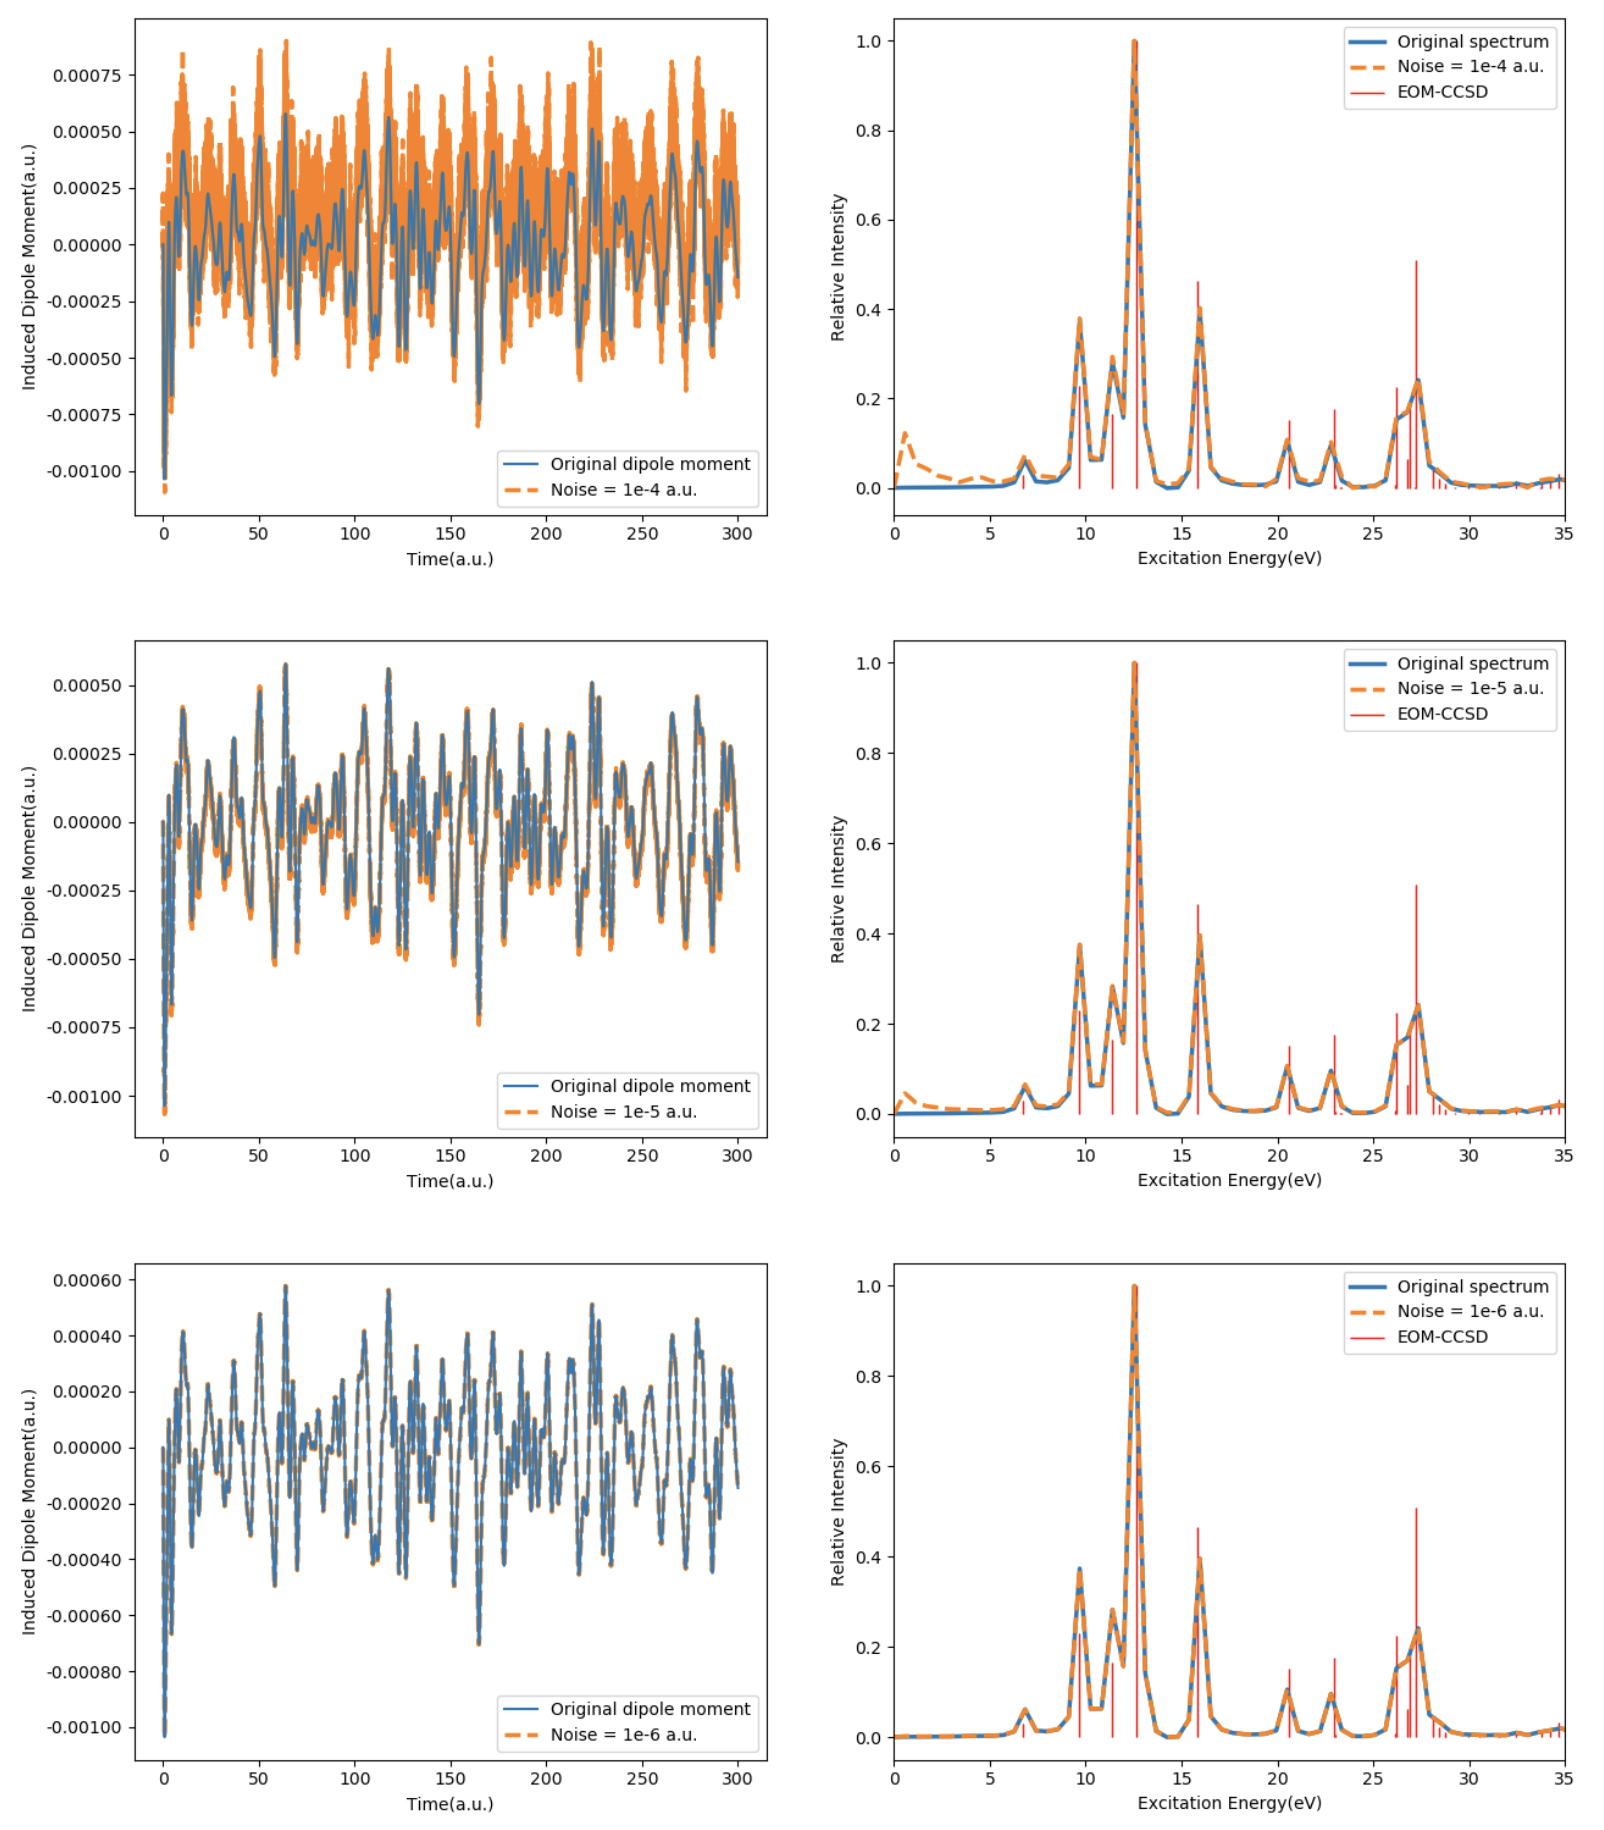
\includegraphics[angle=0, scale=0.4]{ch3/Figs/1-5.png}
    \caption{RT-CCSD/cc-pVDZ time-dependent induced electric dipole moments (left-hand
column) for a water molecule in the presence of an external electric field and
the corresponding linear absorption spectrum (right-hand column) with and
without random noise of varying magnitudes. Corresponding EOM-CCSD/cc-pVDZ 
transitions are included as stick-spectra for comparison.}
    \label{fig:sp-noise}
\end{figure}

To compare the double-precision and single-precision arithmetic directly, we
calculated the RT-CCSD/cc-pVDZ dipole trajectories and corresponding linear
absorption spectra shown in Fig.~\ref{fig:sp-spectrum} using both representations for the series of (H$_2$O)$_n$
clusters with $n=1-4$. For these simulations, the explicit integration was
carried out using the Runge-Kutta 4th order integrator (RK4) with a step size
$h=0.01$ a.u.  The external field was chosen to be a Gaussian envelope defined
in Eq.~(\ref{eq:field}) with ${\cal E} = 0.01$ a.u., $\nu=0.05$ a.u., and
$\sigma=0.01$ a.u. (a narrow pulse). The results are aligned with the numerical
experiments above, with no discernible difference in the spectra after lowering
the arithmetic precision to single-precision. All the spectra are also compared
with EOM-CCSD/cc-pVDZ calculations: we include 40 EOM-CC roots in each of the
spectra, all of which are well-aligned with the associated RT-CC peaks. From this perspective,
the computation time and the required size of memory can both be reduced by
ca.\ a factor of two for the calculation of the spectra, as previously observed
for electronic energies and other components of quantum chemical
calculations.\cite{Ufimtsev2008,Ufimtsev2008quantum,Asadchev2012,Tornai2019,Pokhilko2018}
We note, however, that single-precision arithmetic may not be practical for certain numerically sensitive calculations,
\textit{e.g.}, using higher-order numerical differentiation to extract linear and nonlinear response functions as reported
by Ding \textit{et al.}\cite{Ding2013}
(In addition, we note that these spectra are not intended to reproduce vapor-phase experimental
measurements, only to test the validity of the single-precision arithmetic
approximation.  Thus, any transitions appearing above the physical ionization
limit are not physically realistic and are merely an artifact of the use of a
finite basis set without representation of continuum states.)

\begin{figure}
     \centering
     \begin{subfigure}{0.475\textwidth}
         \centering
         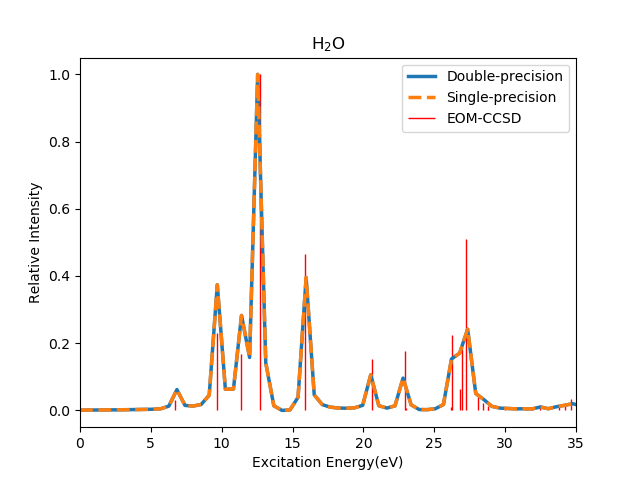
\includegraphics[width=\textwidth]{ch3/Figs/1-1.png}
         \label{fig:sp-monomer}
     \end{subfigure}
     \hfill
     \begin{subfigure}{0.475\textwidth}
         \centering
         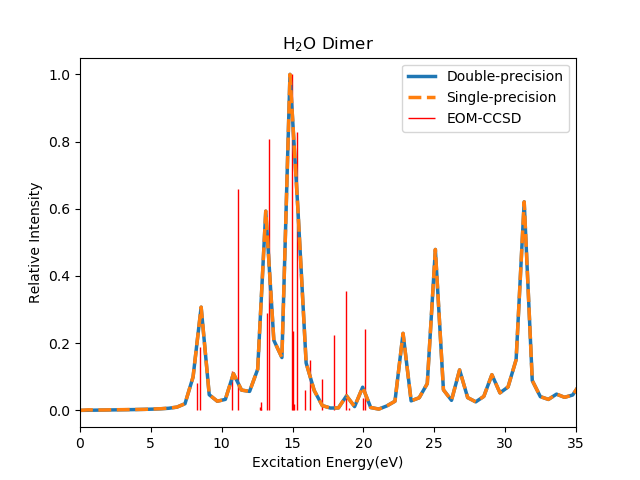
\includegraphics[width=\textwidth]{ch3/Figs/1-2.png}
         \label{fig:sp-dimer}
     \end{subfigure}
     \vfill
     \begin{subfigure}{0.475\textwidth}
         \centering
         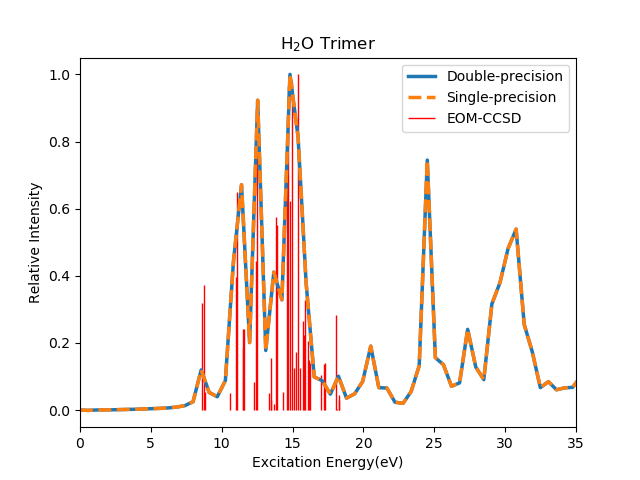
\includegraphics[width=\textwidth]{ch3/Figs/1-3.png}
         \label{fig:sp-trimer}
     \end{subfigure}
     \hfill
     \begin{subfigure}{0.475\textwidth}
         \centering
         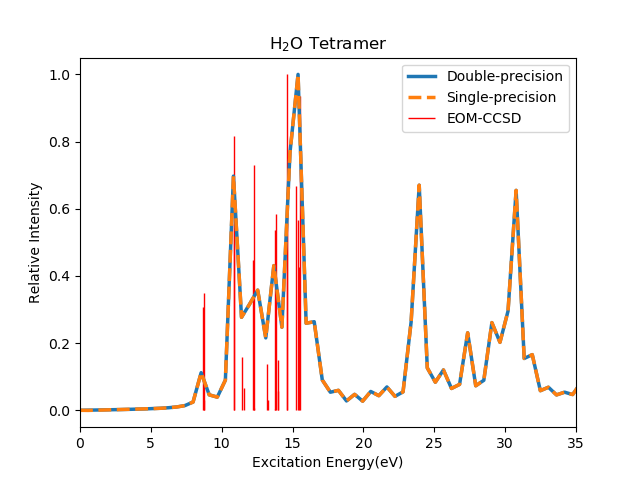
\includegraphics[width=\textwidth]{ch3/Figs/1-4.png}
         \label{fig:sp-tetramer}
     \end{subfigure}
     \caption{Linear UV/vis absorption spectra of (H$_{2}$O)$_n$ clusters for
$n=1-4$ calculated at the RT-CCSD/cc-pVDZ level of theory in both double- and
single-precision arithmetic. Time propagation was carried out for 300 a.u. in
the presence of a weak electric field represented by a narrow Gaussian pulse.
Corresponding EOM-CCSD/cc-pVDZ transitions are included as stick-spectra for
comparison.}
     \label{fig:sp-spectrum}
\end{figure}

Inspired by many parallel implementations of CC methods for distributed memory
architectures on CPUs\cite{Olson2007, Solomonik2014, Janowski2007,
Anisimov2014}, corresponding GPU implementations have become desirable in order
to take advantage of heterogenous artchitectures on modern high-performance
computing systems.  While early GPU hardware was designed for accelerating image
processing with an emphasis on mostly single- or low-precision floating point
operations for quick memory access when higher accuracy is not required, over
the past several years, GPUs have been more extensively used for scientific
research.  In addition to the development of GPUs with robust performance for
double-precision arithmetic, numerous software toolkits have also emerged such
as the Computer Unified Device Architecture (CUDA),\cite{cuda} the Open
Computing Language (OpenCL),\cite{Stone2010} and a variety machine-learning
packages that support GPUs such as TensorFlow,\cite{tensorflow2015}
PyTorch,\cite{Paszke2019} and others, all of which lower the barriers to a wide
range of scientific applications that can take advantage of modern GPU
performance.  We note that, even though the performance of double-precision
calculations on GPUs is already relatively robust, single-precision arithmetic
is still preferable if it provides neglible errors relative to double-precision
results due to the substantial improvement in computational speed and memory
usage.  

For the RT-CC methods explored in this work, we have therefore developed a
GPU-capable implementation within the PyCC code using the PyTorch
package\cite{Paszke2019} based on the conventional CPU version described in
section~\ref{comp}.  In the PyCC implementation, all one-electron quantities
such as the Fock matrix (including the external field), $\hat{T}_1$, and
$\hat{T}_2$ amplitudes are loaded onto the GPU at the beginning of either each
iteration of the time-independent wave function or each computation of the
residuals in Eqs.~(\ref{Eq:derivT}) and (\ref{Eq:derivL}) during the RT-CC
propagation.  As each term in the CC equations is evaluated, the necessary
subblock of the two-electron repulsion integrals is loaded onto the GPU, and the
required tensor contraction is carried out using the usual {\tt opt\_einsum}
function.  Other two- and four-index intermediates formed from the
similarity-transformed Hamiltonian (\textit{e.g.}, the $W_{mbej}$ or $W_{amef}$
intermediates), are retained on the GPU as they are created for later use in the
same iteration/time-step, and deleted once the current residual is complete.
The advantage of this approach is that it provides straightforward access to
local GPU hardware without significant modification of the NumPy-based
tensor-contraction code already in place.  Of course, this Python-based
implementation does not represent the full performance of a production-level
code and is necessarily limited in terms of the size of the molecular system it
can treat, but it does provide a valuable estimate of the minimum expected
speed-up one can obtain for a more highly optimized alogrithm.

Table~\ref{tab:gpu-cpu} provides a comparison of RT-CCSD/cc-pVDZ timings for
double-precision (dp) and single-precision (sp) on CPUs and GPUs for our set of
example water clusters, using the same Gaussian envelope parameters are for
previous computations.  The first three columns report the number of seconds
required for each time step of the RT-CC simulation averaged over a 300 a.u.
propagation (\textit{i.e.}, for a step size of $h=0.01$ a.u., averaged over
30,000 time steps).  As the size of the molecular system increases from monomer
to tetramer, the computational cost per iteration for a CPU-dp calculation
increases by approximately a factor of ca.\ $4^{4.85}$, whereas for a GPU-dp
calculation, the increase is a factor of ca.\ $4^{3.18}$, and for a GPU-sp
calculation, this falls to $4^{2.88}$.  While these are clearly less than the
formal ${\cal O}(4^6)$ scaling expected from CCSD, all of these implementations
would eventually reach that limit for larger systems, because the CPU/GPU and
dp/sp improvements only affect the prefactor, and not the exponent.
Nevertheless, the use of the GPU coupled with single-precision arithmetic
clearly offers substantial advantages.  This improvement is also clearly seen in
the data reported in the final two columns of Table~\ref{tab:gpu-cpu}, where the
single-precision code yields roughly the expected factor of two speed-up over
its double-precision counterpart (with both calculations taking place on the
GPU), and the GPU offers up to a factor of 14 speed-up over the CPU when both
operate in double-precision (or better when the GPU operates in single-precision
mode).  Larger molecular systems should offer even greater improvement, with the
proviso that the memory limits of the GPU will eventually produce a performance
pleateu.
\begin{table} 
    \centering
        \caption{Performance comparison of conventional RT-CC/cc-pVDZ calculations
for water clusters using double-precision on the CPU (CPU-dp), double-precision
on the GPU (GPU-dp), and single-precision on the GPU (GPU-dp). Timings (first
three columns) are given in seconds as per-iteration averages over a 300 a.u.
propagation wth $h=0.01$ a.u.  The final two columns are speed-ups,
\textit{i.e.} ratios of timings for each case.}
    \begin{tabular}{c|ccccc}
       \textrm{Water Cluster} & $t_\textrm{CPU-dp}$ &  $t_\textrm{GPU-dp}$ &
$t_\textrm{GPU-sp}$ & $\frac{t_\textrm{CPU-dp}}{t_\textrm{GPU-dp}}$ &
$\frac{t_\textrm{GPU-dp}}{t_\textrm{GPU-sp}}$\\ \hline
       \textrm{Monomer} & 0.17217 & 0.14330 & 0.13253 & 1.2015 & 1.0813\\ 
       \textrm{Dimer} & 3.4705 & 0.60738 & 0.40496 & 5.7139 & 1.4999\\
       \textrm{Trimer} & 32.729 & 3.4910 & 1.7264 & 9.3752 & 2.0221 \\
       \textrm{Tetramer} & 167.43 & 11.727 & 7.2215 & 14.277 & 1.6239\\     
    \end{tabular}
    \label{tab:gpu-cpu}
\end{table}
        
\subsection{Comparison of Numerical Integrators for RT-CC} \label{result:integrator}

As discussed in section~\ref{theory}, the family of Runge-Kutta methods is the
most widely used class of numerical integrators for IVPs such as the TDSE, not
only because their implementation is straightforward --- \textit{e.g.}, for
RT-CC methods they are easily adapted to accept function vectors taken from the
left- and right-hand wave function residuals in Eqs.~(\ref{Eq:derivT}) and
(\ref{Eq:derivL}) --- but also because of their relatively robust performance
for a range of applications.  The classic Runge-Kutta 4th order integrator
(RK4), for example, is one of the most commonly used algorithms for scientific
problems because it averages each time step into four simple stages and yields a
small truncation error of order $h^{5}$, where $h$ is the step size,
\begin{equation}\label{eq:rk4truncation}
y_{n+1} = y_{n} + \frac{1}{6}(k_{1}+2k_{2}+2k_{3}+k_{4}) + \textit{O}(h^{5}).
\end{equation}

Such explicit integrators typically yield stable propagations of real-time
methods, provided sufficient care is taken in choosing the step size, which is
critical not only for the integration to be numerically stable, accurate, and
efficient, but also cost effective: larger step sizes reduce the computational
expense of the simulation, but they can also result in failure of the
propagation due to a non-convergent time series.  Rather than running sets of
numerical experiments to find the largest, reasonable step size that can provide
accurate results for every application, adaptive integrators\cite{Press1992}
were designed to balance the required stability with the least computational
cost by exerting algorithmic control over step size  within the existing process of
explicit integrators.  For example, Fehlberg\cite{Fehlberg1968} discovered that,
by carrying out six function evaluations per time step and using different
combinations of the six resulting intermediates to formulate a fifth-order
solution and a fourth-order solution, a fourth-order method can be derived with
step size control.  In 1990, Cash and Karp\cite{Cash1990} found another
combination of Fehlberg's coefficients that yields an even more efficient
method,
\begin{equation}\label{eq:ck-k}
\begin{aligned}
k_{1} &= f(t_{n}, y_{n})\\
k_{2} &= f\left(t_{n}+\frac{1}{5}h, y_{n}+\frac{1}{5}k_{1}h\right)\\
k_{3} &= f\left(t_{n}+\frac{3}{10}h,
y_{n}+h\left(\frac{3}{40}k_{1}+\frac{9}{40}k_{2}\right)\right)\\
k_{4} &= f\left(t_{n}+h,
y_{n}+h\left(\frac{3}{10}k_{1}+\frac{9}{10}k_{2}+\frac{6}{5}k_{3}\right)\right)\\
k_{5} &= f\left(t_{n}+\frac{3}{5}h,
y_{n}+h\left(\frac{-11}{54}k_{1}+\frac{5}{2}k_{2}-\frac{70}{27}k_{3}+\frac{35}{27}k_{4}\right)\right)\\
k_{6} &= f\left(t_{n}+\frac{7}{8}h,
y_{n}+h\left(\frac{1631}{55296}k_{1}+\frac{175}{512}k_{2}-\frac{575}{13824}k_{3}+\frac{44275}{110592}k_{4}+\frac{253}{4096}k_{5}\right)\right),
\end{aligned}
\end{equation}
with the resulting coupled time steps being,
\begin{equation}\label{eq:ck-y}
\begin{aligned}
y_{1} &=
y_{n}+h\left(\frac{37}{378}k_{1}+\frac{250}{621}k_{3}+\frac{125}{594}k_{4}+\frac{512}{1771}k_{6}\right)\\
y_{2} &=
y_{n}+h\left(\frac{2825}{27648}k_{1}+\frac{18575}{48384}k_{3}+\frac{13525}{55296}k_{4}+\frac{277}{14336}k_{5}+\frac{1}{4}k_{6}\right)
\end{aligned}
\end{equation}
where $y_{1}$ is a fourth-order solution embedded with $y_{2}$, which is a
fifth-order solution. Therefore, with $\Delta=|y_{2}-y_{1}|$ taken to be an
error estimate for the current time step of order $h^{5}$, a desired accuracy of
$\epsilon$ yields a formula for adjusting the step-size on the fly,
\textit{viz.},
\begin{equation}\label{eq:ck-h}
\frac{h_{new}}{h}=\left(\frac{\epsilon}{\Delta}\right)^{1/5}.
\end{equation}
Thus, if $\Delta$ is smaller than $\epsilon$, $h$ will be increased for the next
step, but if $\Delta$ is larger than $\epsilon$, $h$ will be reduced and the
current step must be repeated until the required accuracy is reached.
Furthermore, if $h$ is reduced and used for the current step again, the error
will have an implicit scaling of $h$, and the exponent in Eq.~(\ref{eq:ck-h})
must be shifted from $\frac{1}{5}$ to $\frac{1}{4}$. The size control of final
step is given as,
\begin{equation}\label{eq:ck-h-final}
\begin{aligned}
h_{new} &= 0.84 h \left(\frac{\epsilon}{\Delta}\right)^{1/5}   \hspace{0.5cm}&
\textrm{for} \hspace{0.1cm}|\Delta| \leq \epsilon \\
h_{new} &= 0.84 h \left(\frac{\epsilon}{\Delta}\right)^{1/4}   \hspace{0.5cm}& 
\textrm{for} \hspace{0.1cm}|\Delta| > \epsilon 
\end{aligned}
\end{equation}
where the coefficient $0.84$ is a ``safety factor'' because the error
estimates are not exact.  Thus, the computational cost of the adaptive
integrator is optimized under a predetermined desired accuracy. If the values at
consecutive time steps change rapidly, a small step size will naturally be used;
if the values vary only slightly, larger step sizes will be sufficient for a
stable propagation. 

In our RT-CC calculations, the time-dependent cluster amplitudes change rapidly
when the external field is on at the beginning of the simulation and gradually
stabilize after the field is turned off.  With this in mind, we tested the
adaptive Cash-Karp (CK) integrator described above for the RT-CCSD simulation
of the absorption spectrum of a single water molecule using the same external
field as in the calculations in section \ref{result:precision}. Additionally,
with the results shown in section \ref{result:precision}, all the calculations
are run in single-precision for the efficiency. 

Fig.~\ref{fig:ck-step} reports the variation in the step size at each iteration
of the propagation using an initial step size of $h=0.01$ a.u.  From
Eq.~(\ref{eq:field}), if $t=0.01$ a.u.\ the field strength is only $3.35\times
10^{-6}$ a.u., and the local error $\Delta$, is expected to be smaller than
$\epsilon$ according to Eq.~(\ref{eq:ck-h-final}), leading to an increase in
$h$ to 0.015 a.u.  At the second time step when $t=0.025$ a.u., the
corresponding field strength is $4.39\times 10^{-4}$ a.u., which gets closer to
its peak of 0.01 a.u.  At this point in the simulation, $\Delta$ is large, and
the CK algorithm automatically reduces the step size to $h=0.012$ a.u.  At the
third and fourth time steps, $h$ slightly increases to 0.014 a.u., because,
even though the field is still on, $h=0.012$ a.u. is small enough to keep
$\Delta$ smaller than $\epsilon$. After the fifth time step, $h$ is increased
to 0.018 a.u. and further 0.027 a.u. when $t=0.064 ~\textrm{to}~ 0.082$ a.u.,
because, during this point in the propagation, the field strength has already
begun to decrease due to the brevity of the pulse.  When the propagation
reaches $t=0.109$ a.u., the magnitude of the field strength falls back to
$10^{-10}$, $\Delta$ is small when $h=0.027$ a.u.\ is tested, and thus $h$
increases to 0.032 a.u.\ at the seventh time step and 0.057 a.u.\ at the eighth
time step. Starting from the ninth time step when $t=0.198$ a.u., although the
external field is essentially zero for the remainder of the propagation, the
algorithm still converges to a step size of $h=0.02$ a.u. due to the continued
oscillation of the amplitudes instigated by the pulse. Since the step size varies 
throughout the propagation, the dipole moments are not calculated at equally 
spaced time points, typical Fourier transform will not work, instead, we pre-process 
our data by interpolating the data points to an evenly spaced grid. Ultimately, after a 300
a.u.\ propagation, the adaptive CK integrator yields an overall speedup of 1.32
relative to the explicit RK4 integrator, yet, as shown in
Fig.~\ref{fig:ck-results}, the final absorption spectra obtained from each
algorithm exhibit no significant differences.  Thus, adaptive integrators such
as the CK algorithm can provide an automated approach to systematically
optimizing the step size depending on the system.

\begin{figure}
    \centering
    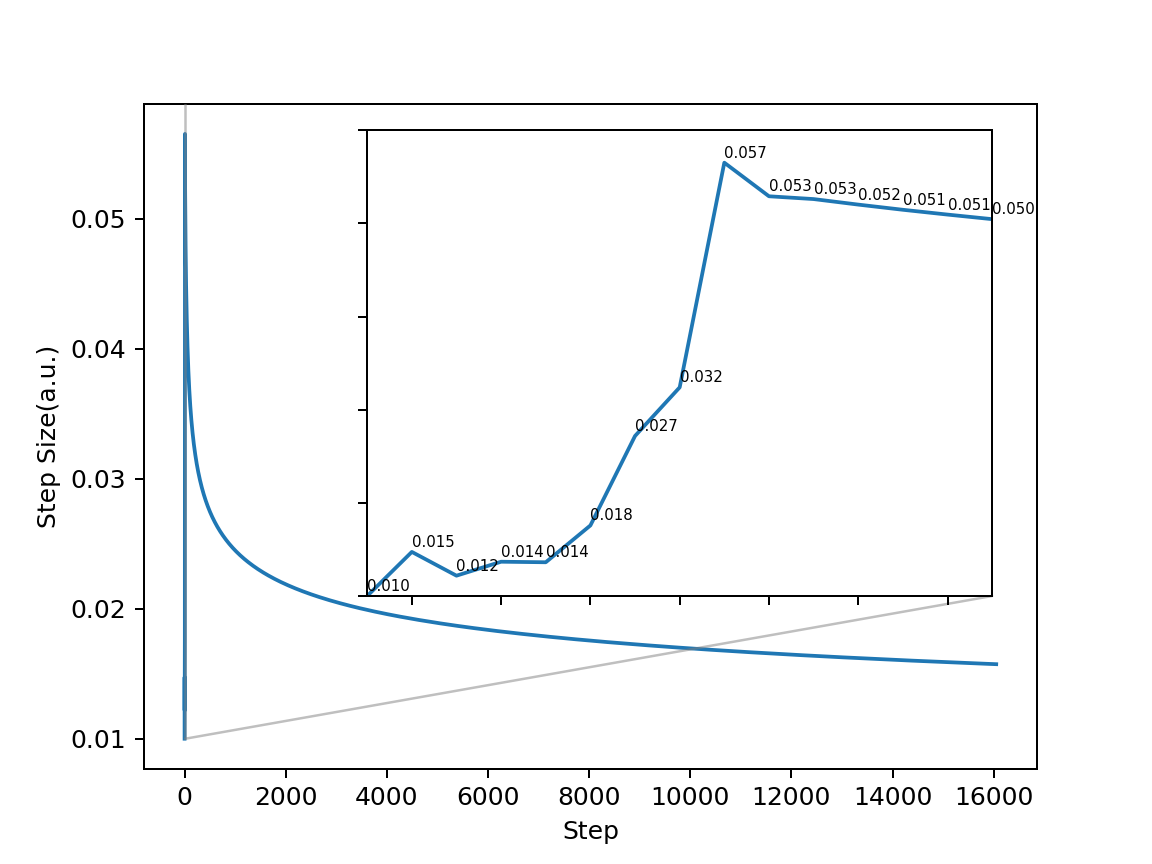
\includegraphics[angle=0, scale=0.3]{ch3/Figs/3-3_new.png}
    \caption{The adjusted step size at each time step in the RT-CCSD/cc-pVDZ
calculation for H$_2$O using the adaptive Cash-Karp integrator over 300 a.u.\
propagation. The first 15 time steps are zoomed in to focus on the detailed change.}
    \label{fig:ck-step}
\end{figure}

\begin{figure}
    \centering
    \begin{subfigure}{0.475\textwidth}
        \centering
        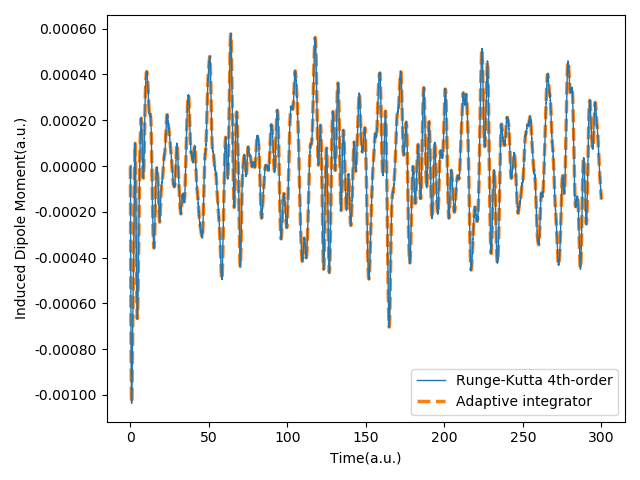
\includegraphics[width=\textwidth]{ch3/Figs/3-1.png}
    \end{subfigure}
    \hfill
    \begin{subfigure}{0.475\textwidth}
        \centering
        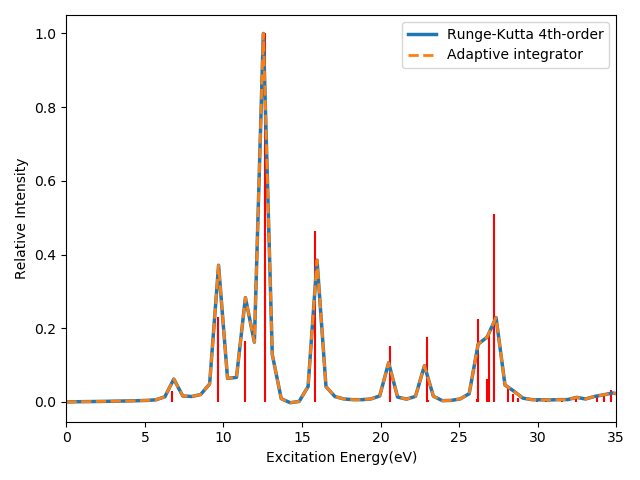
\includegraphics[width=\textwidth]{ch3/Figs/3-2.png}
    \end{subfigure}
    \caption{Comparison of the time-dependent induced dipole moment and the
corresponding linear absorption spectrum from the RT-CCSD/cc-pVDZ simulation of
H$_2$O using RK4 and CK integrators. EOM-CCSD/cc-pVDZ transition energies are
depicted as stick-spectra for reference.}
    \label{fig:ck-results}
\end{figure}

For strong external fields, the numerical stability of the propagation
becomes challenging because the wave function amplitudes fluctuate rapidly
leading to a large local error.  For example, Fig.~\ref{fig:t2-mag} depicts
the norm of the $\hat{T}_2$ amplitudes from an RT-CCSD/cc-pVDZ simulation
of our H$_2$O molecule at several different field strengths of the Gaussian
pulse in Eq.~(\ref{eq:field}) across a 1000 a.u.\ propagation using the RK4
integrator and a step size of $h = 10^{-2}$ a.u. On the scale of the
figure, the weaker fields of ${\cal E} = 0.01$ and $1.0$ a.u.\ induce
relatively small fluctuations in the amplitudes, while a $10.0$ a.u.\ field
yields much larger oscillations.  When the field strength is increased to
${\cal E} = 100.0$ a.u.\, the fluctuations are so great that the
propagation diverges. (This divergence affects both $\hat{T}$- and $\hat{\Lambda}$-amplitudes similarly.) In such cases, the TDSE is commonly referred to as a
``stiff equation'' in that the chosen step size must be extremely small to
maintain the stability of the propagation.  For our ${\cal E} = 100.0$
a.u.\ test case, we find that a step size of $h = 10^{-5}$ a.u.\ is
necessary to maintain the integrity of the simulation, which is clearly
impractical for realistic applications.

\begin{figure}
    \centering
    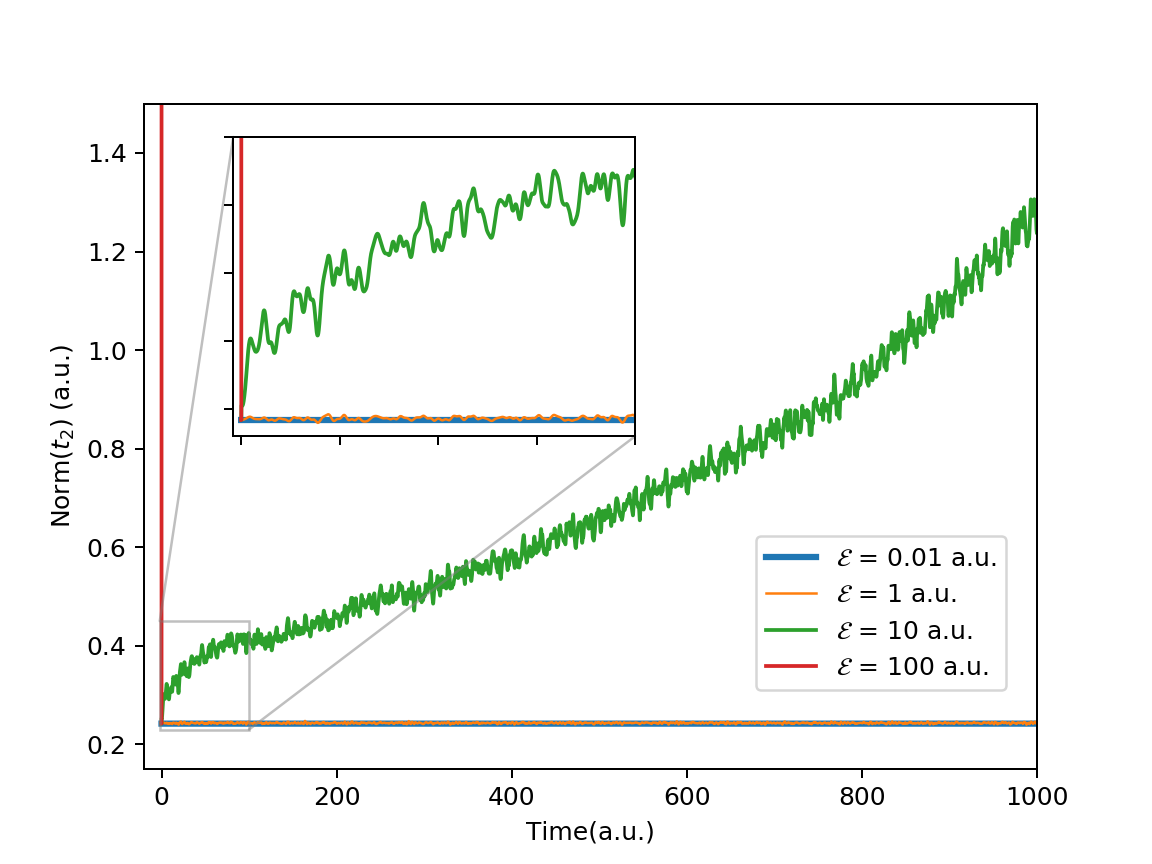
\includegraphics[angle=0, scale=0.3]{ch3/Figs/4-4.png}
    \caption{Comparison of the norm of $\hat{T}_2$ amplitudes during an
RT-CC/cc-pVDZ simulation for H$_2$O using a short Gaussian pulse and the RK4
integrator for different field strengths, ${\cal E}$.}
    \label{fig:t2-mag}
\end{figure}

For the strong-field simulation, it is noteworthy that the divergence
begins near the peak of the of the Gaussian pulse, suggesting that one
might need only decrease the step size while the field is on (the ``bumpy''
portion of the trajectory) and shift to larger values once the field has
decayed.  We therefore carried out a test simulation using $h_1 = 10^{-5}$
a.u.\ when the field is non-zero and $h_2 = 0.01$ a.u.\ otherwise.  The
overhead of this approach is obviously the number of additional residual
evaluations necessary during the pulse, $\frac{\Delta t}{h_{1}} -
\frac{\Delta t}{h_2}$, where $\Delta t$ is the duration of the
field.  The goal is to use steps from $t_{0}$ to $t_{f}$ to track the
interaction with the field precisely, while still minimizing the
computational cost for the overall propagation. 

In order to test this approach, we chose a very narrow Gaussian pulse with
$\nu=0.0005$ a.u.\ and $\sigma=0.0001$ a.u.\ according to the magnitude of
$h_{1}$, once again for an RT-CCSD/cc-pVDZ calculation for a single H$_2$O
molecule, but for a 1000 a.u.\ propagation.  For ${\cal E} = 100.0$ a.u.\
we found that the proposed mixed-step-size approach recovered a stable
propagation, as shown in Fig.~\ref{fig:ms-results}, whose upper-left-hand
plot depicts the norm of the $\hat{T}_2$ wave function parameters as a
function of time. The amplitude of the oscillation is clearly greater than
that induced by weaker fields, which is expected, but it still does not
diverge throughout the propagation. The corresponding absorption spectrum
in the lower-right-hand plot of Fig.~\ref{fig:ms-results} is nearly the
same as that produced by a weaker field in Fig.~\ref{fig:ck-results}, apart
from some additional noise in the low-frequency regime.

\begin{figure}
    \centering
    \begin{subfigure}{0.475\textwidth}
        \centering
        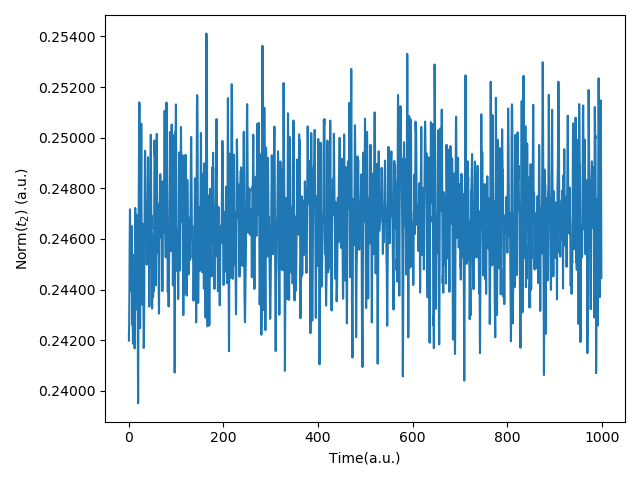
\includegraphics[width=\textwidth]{ch3/Figs/4-5.png}
    \end{subfigure}
    \hfill
    \begin{subfigure}{0.475\textwidth}
        \centering
        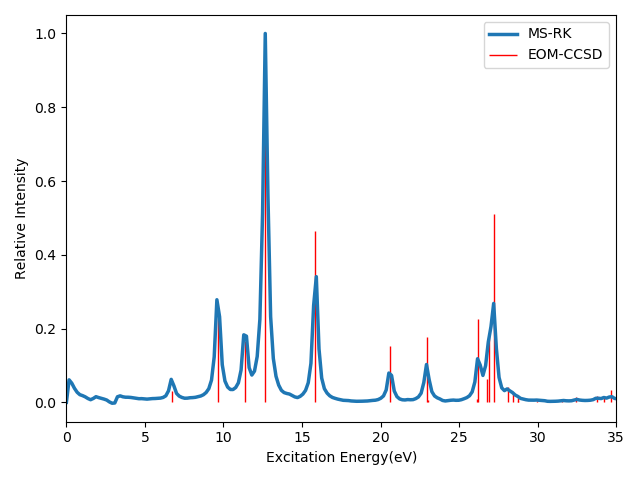
\includegraphics[width=\textwidth]{ch3/Figs/4-3.png}
    \end{subfigure}
    \\
    \begin{subfigure}{0.475\textwidth}
        \centering
        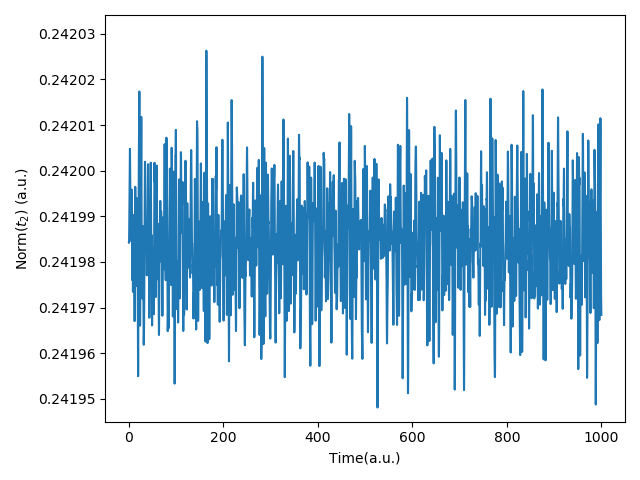
\includegraphics[width=\textwidth]{ch3/Figs/4-6.png}
    \end{subfigure}
    \hfill
    \begin{subfigure}{0.475\textwidth}
        \centering
        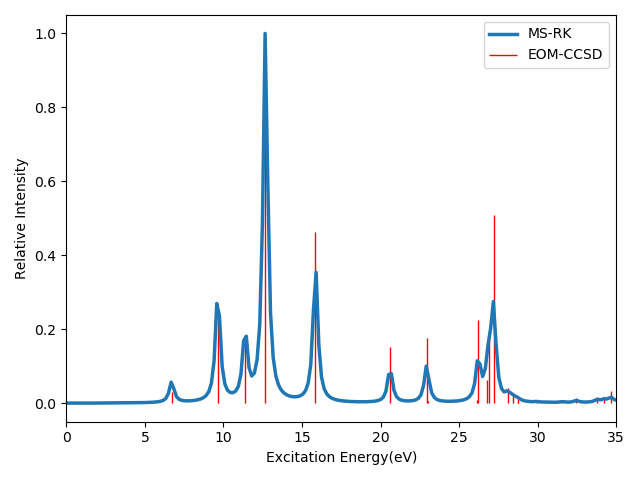
\includegraphics[width=\textwidth]{ch3/Figs/4-7.png}
    \end{subfigure}
    \\
    \begin{subfigure}{0.475\textwidth}
        \centering
        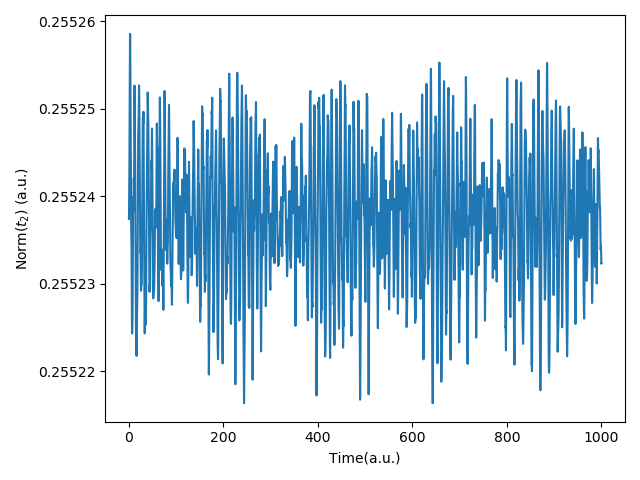
\includegraphics[width=\textwidth]{ch3/Figs/4-8.png}
    \end{subfigure}
    \hfill
    \begin{subfigure}{0.475\textwidth}
        \centering
        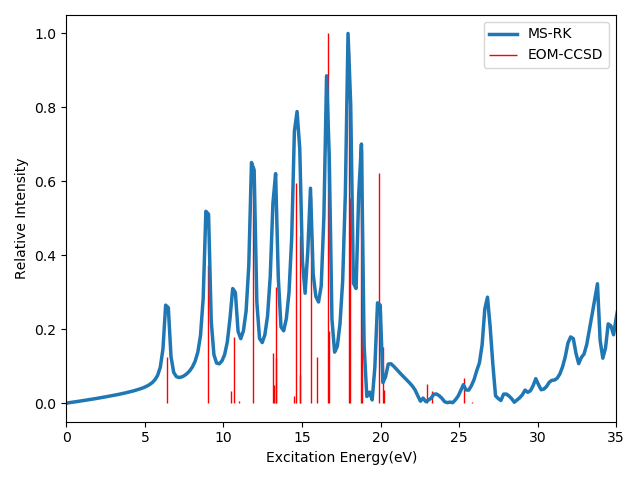
\includegraphics[width=\textwidth]{ch3/Figs/4-9.png}
    \end{subfigure}

    \caption{A $t=1000$ a.u.\ simulation of H$_2$O in the presence of a
    strong ${\cal E} = 100.0$ a.u.\ field with a width of $10^{-4}$ a.u.\
    (upper plot) and $10^{-6}$ a.u.\ (middle plot) at the RT-CCSD/cc-pVDZ
    level of theory using a mixed time-step RK4 approach. The bottom plot differs only from the middle calculation in
    that the aug-cc-pVDZ basis set was used, thus demonstrating that diffuse functions do not affect the numerical
    stability of this simulation.
    The norm of the
    $\hat{T}_2$ amplitudes in each case is depicted in the left-hand plots, and the
    absorption spectrum is shown on the right.}
\label{fig:ms-results}
\end{figure} 

The low-frequency noise disappears, however, if we also choose an even
narrower Gaussian pulse (so as to approximate a strong-field Dirac-delta
pulse) in conjunction with the mixed step-size approach described above.
To demonstrate this we chose parameters for the external field to be
$\cal{E} = 100$ a.u., $\sigma = 10^{-6}$ a.u. and $\nu = 5\times10^{-6}$
a.u.\ with a corresponding step size of $h_{1} =10^{-7}$ a.u.\ during the
pulse and the usual $h_{2} =0.01$ a.u.\ is used after field is off. (Note
that we carried out this calculation in single-precision, and thus
$10^{-7}$ is the smallest scale that can be selected to retain the required
accuracy.) As shown in the middle plots of Fig.~\ref{fig:ms-results}, the
even smaller step size (compared to $h=10^{-5}$ a.u.) gives rise to a more
stable propagation, and therefore, a higher-quality spectrum that avoids
the extra noise in the low-frequency range that appears in the upper-right
panel of Fig.~\ref{fig:ms-results}.  It should also be noted that the
overhead of this calculation is the same as the one with a wider Gaussian
pulse since the ratio $\frac{\Delta t}{h_{1}}$ is unchanged.  Furthermore,
while a mixed step-size approach will necessarily incur more overhead for
more comples field shapes, the stability offered by the algorithm may be
worth the additional expense. Finally we note that, while further testing is necessary to determine the robustness of this
approach across a range of molecular systems, the propagation is stable even for the same molecule and the aug-cc-pVDZ
basis set and with the oxygen $1s$-core electrons included in the correlation treatment. The simulation with aug-cc-pVDZ
basis set is shown in the lower plots of Fig.~\ref{fig:ms-results}.




%conc.tex%
\section{Conclusions} \label{conc}

In this work, we have explored several approaches for improving the
efficiency of the real-time coupled cluster singles and doubles method.
Through a number of numerical experiments on absorption spectra of small
clusters of water molecules, we have found that lowering the arithmetic
representation of the wave function from double- to single-precision yields
negligible differences in the resulting spectra, but speeds up the
calculations by nearly a factor of two compared to the conventional
double-precision implementation.  We have additionally found that migration
of the data and the corresponding tensor contractions from CPU to GPU
utilizing the the PyTorch framework produces a further overall speedup of a
factor of 14.  Based on the rapidly growing computational power of GPU
hardware and their supporting software ecosystem, we intend to carry out
further investigation and optimization of our GPU implementation for
calculations on larger molecular systems. 

We have also investigated a variety of numerical integration schemes for
improving the stability and efficiency of the RT-CC approach, especially
focusing on adaptive integrators that can adjust the step size during the
time-propagation.  In particular, we demonstrate that the Cash-Karp
integrator, which uses an estimate of the local error in each iteration, can
accordingly adjust the time-step to optimize the simulation in terms of
both computing time and numerical stability.  However, for very strong
external fields, such as a narrow Gaussian envelope or delta-pulse, both of
which are commonly used in such simulations, we find that even a
straightforward mixed-step integrator based on the fourth-order Runge-Kutta
algorithm is capable of providing a stable propagation provided a small
enough step size is used in for the duration of the field.  Such an
algorithm should be quite favorable for such calculations with intense, but
narrow laser pulses since it enables the existing RT-CCSD method to be
generally used without any substantial modification to the algorithm or
excessively increased computational cost. While further tests are required to determine the generality and robustness of
this approach, the current results are encouraging.



    \chapter{Real-Time Coupled Cluster Method with Approximate Triples: the Calculation of Optical Properties and Electron Dynamics} \label{ch-4}
\section{Introduction} \label{ch4-intro}
Coupled cluster (CC) theory\cite{Purvis1982, Crawford2000} has been proven to be one of the most accurate and robust correlated methods. The non-truncated CC method that contains all levels of excitations is equivalent to full configurational interaction (CI)\cite{Sherrill1999} and recovers the exact wave function. However, only truncated CC methods are feasible in practical applications, while they still suffer from polynomial scaling. For instance, CCS, CCSD,\cite{Purvis1982} CCSDT,\cite{Noga1987, Scuseria1988} and CCSDTQ\cite{Kucharski1998} scale at $N^{4}$, $N^{6}$, $N^{8}$, and $N^{10}$, respectively. 

Although the inclusion of singles and doubles has been widely used and affirmed to be effective and efficient, a higher level of theory is still in demand to achieve a closer comparison to full CI and/or recover missing properties. Covering triple excitation operators is an obvious starting point. It needs to be pointed out that triple excitations can already be obtained from lower excitation operators in CC by definition. For instance, the coupled cluster singles and doubles (CCSD) method can introduce triple excitations by having terms like $\hat{T}_{1}\hat{T}_{2}$ and $\hat{T}_{1}^{3}$. It is important to figure out which are the leading terms among all triple excitations and wether the addition of the triple excitation operator $\hat{T}_{3}$ is key to the problem, as it indeed sacrifices the computational efficiency to some extent. To understand this, many-body perturbation theory (MBPT)\cite{Bartlett1981} is a paramount and straightforward technique to show how higher excitations impact the electron-correlation effects and further affect the properties. According to MBPT, $\hat{T}_{3}$ contributes and appears for the first time in the fourth-order correlation energy, while $\hat{T}_{1}\hat{T}_{2}$ and $\hat{T}_{1}^{3}$ first appear in higher orders. Thus, to make a method correct to the fourth order, triples are essential, not only for the correlation energy itself,\cite{Lee1984} but also for other properties, including excitation energies,\cite{Christiansen1995CC3, Watts1995, Christiansen1996, Kucharski2001} polarizabilities,\cite{Christiansen1998triple, Hald2003} NMR parameters,\cite{Gauss1996, Faber2017, Jaszunski2020} and so on.

Over the decades, alternatives to treat triples have been explored, as the full CCSDT is expensive due to summations involving as many as eight indices. Among various techniques, CCSDT-n\cite{Noga1987ccsdtn} models are among the earliest ones that retain only the important terms in the triples equation. They are constructed iteratively, approximating triples based on the single and/or double amplitudes, resulting a scaling of $N^{7}$. In the simplest model, known as the coupled cluster singles, doubles, and linearized triple excitation method (CCSDT-1),\cite{Lee1984, Urban1985} only terms with linearized $\hat{T}_{2}$, which contribute the most to triples, are retained in the $\hat{T}_{3}$ equation. Linearized triples, which can improve the MBPT energy to the fourth order, are further used to solve the $\hat{T}_{1}$ and $\hat{T}_{2}$ amplitudes. This is an equivalent approximation to $e^{\hat{T}_{1}+\hat{T}_{2}} + \hat{T}_{3}$ and is often denoted as CCSDT-1a. On the other hand, CCSDT-1b is defined to be a slightly more accurate model, including all the terms in CCSDT-1a, plus the ones involving the product of $\hat{T}_{1}$ and $\hat{T}_{3}$ in the $\hat{T}_{2}$ equation. Additionally, if $e^{\hat{T}_{2}}$ is preserved in the $\hat{T}_{3}$ equation rather than solely $\hat{T}_{2}$, CCSDT-2\cite{Noga1987ccsdtn} can be formulated to include the non-linear term $\hat{T}_{2}^{2}$. Another extended model, CCSDT-3,\cite{Noga1987ccsdtn} approximates $\hat{T}_{3}$ by using $e^{\hat{T}_{1} + \hat{T}_{2}}$ and improves the accuracy compared to CCSDT-2, especially when $\hat{T}_{1}$ amplitudes are large. 

Apart from these iterative models, the investigation of non-iterative models was motivated by reducing the computational cost. Augmented coupled cluster models, including CCSD+T(CCSD)\cite{Urban1985} and CCSD(T)\cite{Raghavachari1989, Stanton1997} methods, use the converged CCSD parameters and introduce triples in a non-interactive manner by adding dominant terms in the fifth-order perturbation expansion of the correlation energy. The correction gained from the triples is evaluated from CCSD $\hat{T}_{2}$ amplitudes in CCSD+T(CCSD), but from both CCSD $\hat{T}_{1}$ and $\hat{T}_{2}$ amplitudes in CCSD(T). Due to the equal treatment of singles and doubles in CCSD(T), a closer approximation to CCSDT is obtained. In practical implementations, the non-iterative methods have only one step that scales at $N^{7}$, succeeding the CCSD iterations with a scaling of $N^{6}$ while the iterative methods have every iteration scale at $N^{7}$. CCSD(T) is hereby acknowledged as the gold standard in quantum chemistry. Given the success of CCSD(T) for static correlation, the non-interactive manner of introducing triples also leads to a deficiency in calculating time-dependent properties. On the contrary, an approximate coupled cluster singles, doubles and triples (CC3)\cite{Koch1997} model is preferable for such properties. 

CC3 is an iterative model that treats singles uniquely as zero-order parameters for an approximation of orbital relaxation, with triples being correct to the second order. During each iteration, approximate triples are calculated and used for a subsequent calculation of their contributions to the singles and doubles, in order to correct the energy to the fifth order. In this manner, contractions with a scaling of $N^{7}$ occur with the triple amplitudes, but triples need not to be stored, in terms of additional computational cost. Simultaneously, singles and doubles are updated and stored every iteration and returned after convergence, resulting in the same formula for calculating the correlation energy as CCSD.

CC3 can provide comparable results compared to other iterative and non-iterative approximate triples models for time-independent properties.\cite{Koch1997} More crucially, time/frequency-dependent properties, including response functions, can be derived as opposed to CCSD(T).\cite{Koch1997, Christiansen1995CC3} If considered only in comparison with other iterative models, counting singles as zero-order parameters underscores the greater importance of singles for properties related to the perturbation of an external electromagnetic field and excited states. This makes it an exceptional candidate to be combined with, for example, equation-of-motion methods,\cite{Stanton1993} linear response theory,\cite{Olsen1985, Sekino1984} and real-time methods,\cite{Goings2018, Li2020} in order to involve higher excitations.

Here, we propose the first implementation of the RT-CC3 method, which is built upon our existing RT-CC framework. As stated above, the CC3 method works particularly well for dynamic properties arising from the interaction between the system and the external electromagnetic field. For instance, it excels in calculating induced dipole moments due to its iterative construction and the special treatment of single amplitudes.\cite{Hald2002} Calculations of response functions were soon explored alongside the CC3 model itself and were compared with other iterative models such as CCSDT-1a and CCSDT-1b, where CC3 was found to be favorable.\cite{Christiansen1995CC3} The excitation energy of various molecules was significantly improved by CC3 compared to CCSD and was close to CCSDT. Second-order properties, such as polarizabilities, were also obtained from CC3 linear response functions and showed good agreement with experimental data for the tested molecules.\cite{Hald2003} For these reasons, the RT-CC3 method is desirable for calculating these properties, as it combines advantages from both the real-time formalism and the CC3 model.

The calculation of the absorption spectrum is conducted and compared to the equation-of-motion (EOM) CC results to validate the RT-CC3 method. For higher-order properties, instead of using the Fourier transform of the corresponding time-dependent properties, finite-difference methods\cite{Perrone1975} are used to calculate numerical derivatives to obtain properties including polarizabilities, the $G'$ tensor related to optical rotation, hyperpolarizabilities, etc. This approach was first proposed by Ding et al. in an application of real-time time-dependent density functional theory (RT-TDDFT), allowing response properties to be obtained from a group of propagations with different field strengths.\cite{Ding2013} Without the need for explicit Fourier transform, each propagation does not need to be as long as those for obtaining, for example, absorption spectra, where the resolution of the spectra depends on sufficient propagation time. Additionally, properties related to different orders of response to the same field can be calculated using the same group of propagations. The formalism for calculating different orders of numerical derivatives is relatively simple compared to the derivation of linear, quadratic, or even higher-order response functions. Details about the implementation of the finite difference method and the discussion of the accuracy and stability of the RT-CC3 simulation, along with real-time simulations at other levels of theory, will be presented in the later sections.

Besides response properties, another interesting simulation accessible within the RT framework is observing Rabi oscillation,\cite{Knorr1994} which is the oscillation of level population under the influence of an incident light field. A series of discussions on the simulation using RT-TDDFT was published by the Isborn group, focusing on the formulation of the method and addressing false observations due to deficiencies in available exchange functionals.\cite{Habenicht2014, Provorse2015, Provorse2016, Ranka2023} Another application of RT-CC methods on collective Rabi oscillation was conducted by Andreas et al., discussing the differences in quality and stability of the simulation between time-dependent equation-of-motion coupled cluster and time-dependent coupled cluster.\cite{Skeidsvoll2023} In this paper, a simulation of Rabi oscillation is conducted using RT-CCSD, following a discussion on the population of the excited states.




\section{Theory} \label{theory_cc3} 
\subsection{RT-CC3 Method} \label{theory-cc3-1}
\subsubsection{CC3 Model}  \label{theory-cc3-11}
In CC theory, the wave function is represented as 
\begin{equation}
\ket{\Phi_{CC}}=e^{\hat{T}}\ket{\Phi_{0}},
\end{equation}
where $\ket{\Phi_{0}}$ is the single-reference state that is typically chosen to be the Hartree-Fock wave function, and $\hat{T}$ is the cluster operator defined as
\begin{equation}
\hat{T} = \sum_{i=1, 2, ..., N}\hat{T}_{i},
\label{eq:cc3-t}
\end{equation}
with $N$ being the number of electrons of the system. For a closed-shell restricted Hartree-Fock (RHF) formalism, the singles, doubles and triples are written as
\begin{equation}
\hat{T}_{1}=\sum_{ia}t_{i}^{a}a_{a}^{+}a_{i},
\label{eq:cc3-T1}
\end{equation}
\begin{equation}
\hat{T}_{2}=\frac{1}{2}\sum_{ijab}t_{ij}^{ab}a_{a}^{+}a_{b}^{+}a_{j}a_{i},
\label{eq:cc3-T2}
\end{equation}
and
\begin{equation}
\hat{T}_{3}=\frac{1}{6}\sum_{ijkabc}t_{ijk}^{abc}a_{a}^{+}a_{b}^{+}a_{c}^{+}a_{k}a_{j}a_{i},
\label{eq:cc3-T3}
\end{equation}
respectively, where $i, j, k, ...$ are occupied orbitals, and $a, b, c, ...$ are virtual orbitals. The sum of the number of occupied orbitals (NO) and the number of virtual orbitals (NV) equals to the number of molecular orbitals (NMO). From the Schr\"odinger equation of the CC wave function:
\begin{equation}
\hat{H}\ket{\Phi_{CC}}=E_{CC}\ket{\Phi_{CC}}=E_{CC}e^{\hat{T}}\ket{\Phi_{0}},
\end{equation}
the CC energy can be obtained in the form of
\begin{equation}
E_{CC} = \bra{\Phi_{0}}e^{-\hat{T}}\hat{H}e^{\hat{T}}\ket{\Phi_{0}}
\label{eq:cc3-ecc}
\end{equation}
when left projecting the reference state together with the exponential. $e^{-\hat{T}}\hat{H}e^{\hat{T}}$ is usually denoted as the similarity-transformed Hamiltonian $\bar{H}$. If left-projecting the substituted determinant instead, the CC amplitudes can be solved using the equation
\begin{equation}
\bra{\mu_{i}}\bar{H}\ket{\Phi_{0}}=0,
\label{eq:cc3-amp}
\end{equation}
where $i$ is the excitation level. The ground state CC energy is obtained with converged amplitudes from Eq.~(\ref{eq:cc3-amp}). If we take the CC energy as the stationary point and the amplitude equation as the constraint, an energy Lagrangian can be constructed as:
\begin{equation}
\mathcal{L}_{CC} = \bra{\Phi_{0}}\bar{H}\ket{\Phi_{0}} + \sum_{\mu}\lambda_{\mu}\bra{\mu}\bar{H}\ket{\Phi_{0}},
\label{eq:cc3-lag}
\end{equation}
where $\lambda$ is the Lagrangian multiplier. A de-excitation operator $\hat{\Lambda}$, in analogous to the $\hat{T}$ operator, can be defined as
\begin{equation}
\hat{\Lambda}=\sum_{i=1, 2, ..., N}\hat{\Lambda}_{i},
\end{equation}
with
\begin{equation}
\bra{\Phi_{0}}\hat{\Lambda}=\sum_{\mu}\lambda_{\mu}\bra{\mu}
\end{equation}
to serve as additional parameters representing the left-hand eigenvector of $\bar{H}$, which is distinct from the right-hand eigenvector since $\bar{H}$ is not Hermitian. They are equivalent to the Lagrangian multipliers in the Lagrangian formalism. There exists an optimal set of $t's$ and $\lambda's$ that can converge the energy Lagrangian to its minimum. Therefore, the $\hat{T}$ and $\hat{\Lambda}$ amplitude equations can be derived from 
\begin{equation}
\frac{\partial \mathcal{L}_{CC}}{\partial \lambda_{\mu}}=0
\label{eq:cc3-lag-t-eq}
\end{equation}
and
\begin{equation}
\frac{\partial \mathcal{L}_{CC}}{\partial t_{\mu}}=0,
\label{eq:cc3-lag-l-eq}
\end{equation}
respectively.
Although this does not lead to a simpler method of solving the energy itself, it provides a convenient approach to discussing the perturbation expansion of the energy. The the energy Lagrangian can be expanded as 
\begin{equation}
\mathcal{L} = \mathcal{L}^{(0)} + \mathcal{L}^{(1)} + \mathcal{L}^{(2)} + ...,
\end{equation}
also the cluster operators as
\begin{equation}
\hat{T} = \hat{T}^{(0)} + \hat{T}^{(1)}+ \hat{T}^{(2)} + ...
\end{equation}
and
\begin{equation}
\hat{\Lambda} = \hat{\Lambda}^{(0)} + \hat{\Lambda}^{(1)} + \hat{\Lambda}^{(2)} + ...
\end{equation}
From Eqs.~(\ref{eq:cc3-lag-t-eq}) and~(\ref{eq:cc3-lag-l-eq}), the $nth$-order amplitudes can be calculated from
\begin{equation}
\frac{\partial{\mathcal{L}^{(n)}}}{\partial{t_{\mu}^{(n)}}}=0
\label{eq:cc3-partial-lag-t}
\end{equation}
and
\begin{equation}
\frac{\partial{\mathcal{L}^{(n)}}}{\partial{\lambda_{\mu}^{(n)}}}=0.
\label{eq:cc3-partial-lag-l}
\end{equation}
With the knowledge of $\hat{T}$ amplitudes up to the $n$-th order,  the $(2n+1)$-order energy can be calculated, and with the knowledge of $\hat{\Lambda}$ amplitudes up to the $n$-th order, the $(2n+2)$-order energy can be calculated. These rules are known as Wigner's $(2n+1)$ and $(2n+2)$ rules.\cite{Kvasnivcka1980, Shavitt2009} It can be proved that the zeroth-order amplitudes are equal to zero, the first-order amplitudes contain only doubles, and the first non-vanishing order for triples is the second order, as demonstrated in Ref.~\citenum{Koch1997}.

In CC3, only the second-order triples are kept. Singles are treated as the approximate orbital relaxation parameters at the zeroth-order, as opposed to the second-order in MBPT. Applying these conditions to Eq.~(\ref{eq:cc3-lag}) and partitioning the Hamiltonian into the Fock operator $\hat{F}$ and the fluctuation operator $\hat{U}$ results in:
\begin{equation}
\hat{H} =  \hat{F} + \hat{U},
\label{eq:cc3-h}
\end{equation}
the CC3 Lagrangian becomes
\begin{align}
\begin{split}
\mathcal{L}_{CC3} &= \bra{\Phi_{0}}\bar{H}\ket{\Phi_{0}} \\
&+ \sum_{\mu_{1}}\lambda_{\mu_{1}}\bra{\mu_{1}}H + [H, \hat{T}_{2}] + [H, \hat{T}_{3}] \ket{\Phi_{0}} \\
&+ \sum_{\mu_{2}}\lambda_{\mu_{2}}\bra{\mu_{2}}H + [H, \hat{T}_{2}] + \frac{1}{2}[[H, \hat{T}_{2}], \hat{T}_{2}] + [H, \hat{T}_{3}] \ket{\Phi_{0}} \\
&+ \sum_{\mu_{3}}\lambda_{\mu_{3}}\bra{\mu_{3}}[H, \hat{T}_{2}] + [F, \hat{T}_{3}] \ket{\Phi_{0}},
\label{eq:cc3-lag-cc3}
\end{split}
\end{align} 
where the operator $H$ and $F$ represent the $T_{1}$-transformed Hamiltonian and Fock operator, respectively, when a $T_{1}$-transformed operator is defined as
\begin{equation}
O = e^{-\hat{T}_{1}}\hat{O}e^{\hat{T}_{1}}.
\end{equation}
The perturbative order of each term in Eq.~(\ref{eq:cc3-lag-cc3}) can be determined by the perturbative orders of its components. For instance, as $F$ and $U$ are considered to be zeroth- and first-order, respectively, and $\Lambda_{2}$ is considered to be first-order, the term $\sum_{\mu_{2}}\lambda_{\mu_{2}}\bra{\mu_{2}}[U, \hat{T}_{3}]\ket{\Phi_{0}}$ contributes to the fourth-order energy. Similarly, the overall corrections to the fourth- and fifth-order energies are extracted as:
\begin{equation}
 \sum_{\mu_{2}}\lambda_{\mu_{2}}\bra{\mu_{2}}[U, \hat{T}_{3}]\ket{\Phi_{0}} + 
 \sum_{\mu_{3}}\lambda_{\mu_{3}}\bra{\mu_{3}}[H, \hat{T}_{2}] + [F, \hat{T}_{3}]\ket{\Phi_{0}}
  \rightarrow E^{(4)},
\end{equation}
and
\begin{equation}
 \sum_{\mu_{3}}\lambda_{\mu_{3}}\bra{\mu_{3}}[U, \hat{T}_{2}]\ket{\Phi_{0}}
  \rightarrow E^{(5)},
\end{equation}
respectively.

To derive the CC3 $\hat{T}$ amplitude equation, we bring $\mathcal{L}_{CC3}$ from Eq.~(\ref{eq:cc3-lag-cc3}) into Eq.~(\ref{eq:cc3-lag-t-eq}). Then, the equations for $\hat{T}_{1}$, $\hat{T}_{2}$, and $\hat{T}_{3}$ can be written in the form of
\begin{equation}
\bra{\mu_{1}}H + [H, \hat{T}_{2}] + [H, \hat{T}_{3}] \ket{\Phi_{0}}=0,
\label{eq:cc3-t1}
\end{equation}
\begin{equation}
\bra{\mu_{2}}H + [H, \hat{T}_{2}] + \frac{1}{2}[[H, \hat{T}_{2}], \hat{T}_{2}] + [H, \hat{T}_{3}] \ket{\Phi_{0}}=0,
\label{eq:cc3-t2}
\end{equation}
and
\begin{equation}
\bra{\mu_{3}}[H, \hat{T}_{2}] + [F, \hat{T}_{3}] \ket{\Phi_{0}}=0.
\label{eq:cc3-t3}
\end{equation}
Expanding and rearranging terms in Eq.~(\ref{eq:cc3-t3}), triples can be calculated explicitly as 
\begin{equation}
t_{\mu_{3}}= -\frac{\bra{\mu_{3}}[U, \hat{T}_{2}]\ket{\Phi_{0}}}{\epsilon_{\mu_{3}}},
\label{eq:cc3-final-t3}
\end{equation}
where the denominator $\epsilon_{\mu_{3}}$ is the difference between the sum of the virtual orbital energies and the sum of the occupied orbital energies. The $\hat{T}_{1}$ and $\hat{T}_{2}$ equations can also be rewritten as
\begin{equation}
\bra{\mu_{1}} e^{-(\hat{T}_{1}+\hat{T}_{2})}\hat{H}e^{\hat{T}_{1}+\hat{T}_{2}}\ket{\Phi_{0}} +\bra{\mu_{1}}[\hat{H}, \hat{T}_{3}] \ket{\Phi_{0}}=0
\label{eq:cc3-final-t1}
\end{equation}
and
\begin{equation}
\bra{\mu_{2}} e^{-(\hat{T}_{1}+\hat{T}_{2})}\hat{H}e^{\hat{T}_{1}+\hat{T}_{2}}\ket{\Phi_{0}} +\bra{\mu_{2}}[H, \hat{T}_{3}] \ket{\Phi_{0}}=0
\label{eq:cc3-final-t2}
\end{equation}
to separate the CCSD component in the first term and the contribution from the triples in the second term. The contributions to the $\hat{T}_{1}$ and  $\hat{T}_{2}$ amplitudes from the connected triples are defined as
\begin{equation}
X_{1} = \bra{\mu_{1}}[\hat{H}, \hat{T}_{3}] \ket{\Phi_{0}}
\label{eq:cc3-x1}
\end{equation}
and
\begin{equation}
X_{2} = \bra{\mu_{2}}[H, \hat{T}_{3}] \ket{\Phi_{0}}.
\label{eq:cc3-x2}
\end{equation}

When calculating the CC3 ground state energy, all amplitudes are solved iteratively. During each iteration, the approximate $\hat{T}_{3}$ amplitude, which is correct to the second order, is calculated using the  $\hat{T}_{1}$ and  $\hat{T}_{2}$ amplitudes from the previous iteration, as shown in Eq.~(\ref{eq:cc3-final-t3}). Its contribution to the new $\hat{T}_{1}$ and  $\hat{T}_{2}$ amplitudes, $X_{1}$ and $X_{2}$, can be calculated using Eqs.~(\ref{eq:cc3-x1}) and~(\ref{eq:cc3-x2}), and then added to the CCSD amplitude residuals to obtain the $\hat{T}_{1}$ and  $\hat{T}_{2}$ amplitudes for the current iteration. 

To calculate other molecular properties, $\hat{\Lambda}$ amplitudes are calculated by inserting $\mathcal{L}_{CC3}$ into Eq.~(\ref{eq:cc3-lag-l-eq}). The resulting $\hat{\Lambda}$ equations can be organized in matrix form as follows:
\begin{gather}
 \begin{pmatrix} \lambda_{\mu_{1}}&\lambda_{\mu_{2}}&\lambda_{\mu_{3}} \end{pmatrix}
 \textbf{A}
 = -
  \begin{pmatrix}
   \bra{\Phi_{0}} \bar{H}\ket{\mu_{1}}&
   \bra{\Phi_{0}} \bar{H}\ket{\mu_{2}}&
   0
   \end{pmatrix},
\end{gather}
where
\begin{gather}
 \textbf{A} = 
\begin{pmatrix} 
   \bra{\mu_{1}}H + [\hat{H}, \hat{T}_{2}]\ket{\nu_{1}} & \bra{\mu_{1}}H \ket{\nu_{2}} & \bra{\mu_{1}}\hat{H} \ket{\nu_{3}} \\
   \bra{\mu_{2}}H + [H, \hat{T}_{2}]+ [\hat{H}, \hat{T}_{3}]\ket{\nu_{1}} & \bra{\mu_{2}}H + [\hat{H}, \hat{T}_{2}]\ket{\nu_{2}} &  \bra{\mu_{2}} H \ket{\nu_{3}}  \\
    \bra{\mu_{3}} [H, \hat{T}_{2}]\ket{\nu_{1}} &  \bra{\mu_{3}} H \ket{\nu_{2}} & 0
  \end{pmatrix}.
\end{gather}
Similar to $\hat{T}$ equations, only terms involving triples need to be calculated to obtain the $\hat{\Lambda}_{3}$ amplitude itself and its contributions to the $\hat{\Lambda}_{1}$ and $\hat{\Lambda}_{2}$ amplitudes, which are defined as
\begin{equation}
Y_{1} = \bra{\Phi_{0}}\hat{\Lambda}_{2}[\hat{H}, \hat{T}_{3}]\ket{\nu_{1}} + \bra{\Phi_{0}}\hat{\Lambda}_{3}[\hat{H}, \hat{T}_{2}]\ket{\nu_{1}}
\label{eq:cc3-y1}
\end{equation}
and
\begin{equation}
Y_{2} = \bra{\Phi_{0}}\hat{\Lambda}_{3}[H, \hat{T}_{2}]\ket{\nu_{2}}.
\label{eq:cc3-y2}
\end{equation}
The simplified $\hat{\Lambda}_{3}$ equation for the second-order $\hat{\Lambda}_{3}$ amplitudes may be written as
\begin{equation}
\lambda_{\mu_{3}}=-\frac{\bra{\Phi_{0}}\hat{\Lambda}_{1}\hat{H}\ket{\nu_{3}} + \bra{\Phi_{0}}\hat{\Lambda}_{2}H\ket{\nu_{3}}}{\epsilon_{\mu_{3}}}.
\label{eq:cc3-l3}
\end{equation}

Now, if we consider the case where the molecule is subjected to an external perturbation $\beta\hat{V}$, such as an electromagnetic field, where $\beta$ represents the field strength and $\hat{V}$ is the one-electron perturbation operator, the Hamiltonian can be written as follows:
\begin{equation}
\hat{H}  \rightarrow \hat{H} + \beta\hat{V} = \hat{F} + \beta\hat{V} + \hat{U},
\label{eq:cc3-h-pert}
\end{equation}
where $\hat{F}+\hat{U}$ can be seen as the zeroth-order Hamiltonian, and $\beta\hat{V}$ contributes to the first-order energy Lagrangian as the first-order Hamiltonian. If we consider this scenario as the zeroth-order $\hat{F}$ being perturbed by two individual perturbations, $\hat{U}$ and $\beta\hat{V}$, the modified Fock operator $\hat{F}+\beta\hat{V}$ can no longer be treated as zeroth-order. Since CC3 does not involve explicit orbital relaxation, no approximations should be applied to the singles due to their unique role. All terms that involve $\hat{V}$ must be retained, leading to an additional term in the $\hat{T}_{3}$ equation compared to Eq.~(\ref{eq:cc3-t3}). The modified $\hat{T}_{3}$ equation can be written as 
\begin{equation}
t_{\mu_{3}}= -\frac{\bra{\mu_{3}}[U, \hat{T}_{2}]\ket{\Phi_{0}} + \frac{1}{2}\bra{\mu_{3}}[[\beta V, \hat{T}_{2}], \hat{T}_{2}]\ket{\Phi_{0}}}{\epsilon_{\mu_{3}}}.
\label{eq:cc3-final-t3-pert}
\end{equation}
Under the influence of an external perturbation, it becomes possible to calculate properties that arise from its interaction with the system. For example, if the external perturbation is represented by an external electric field, the induced electric dipole moments can be determined. In the case of first-order properties, the expectation value of the corresponding operator can be computed. One convenient approach involves calculating the derivative of the first-order Lagrangian with respect to the field strength, as shown in Eq.~(\ref{eq:cc3-prop1}). Alternatively, the expectation value can be represented as the contraction of the one-electron density $D_{pq}$ and the property integrals $V_{pq}$, as demonstrated in Eq.~(\ref{eq:cc3-prop2}), where $p$ and $q$ represent molecular orbitals. 
\begin{equation}
\langle\hat{V}\rangle = \frac{\partial\mathcal{L}_{CC3}^{(1)}}{\partial\beta}
\label{eq:cc3-prop1}
\end{equation}
\begin{equation}
\langle\hat{V}\rangle = \sum_{pq}D_{pq}V_{pq}
\label{eq:cc3-prop2}
\end{equation}
By equating the right-hand sides of Eqs.~(\ref{eq:cc3-prop1}) and~(\ref{eq:cc3-prop2}), terms for calculating the elements of the one-electron density matrix can be derived. The contribution from triples is highlighted and presented as
\begin{equation}
\bra{\Phi_{0}}\hat{\Lambda}_{2}[E_{pq}, \hat{T}_{3}]\ket{\Phi_{0}} + \bra{\Phi_{0}}\hat{\Lambda}_{3}[E_{pq}, \hat{T}_{3}]\ket{\Phi_{0}} 
+ \frac{1}{2}\bra{\Phi_{0}}\hat{\Lambda}_{3}[[E_{pq}, \hat{T}_{2}], \hat{T}_{2}]\ket{\Phi_{0}} \rightarrow D_{pq},
\label{eq:cc3-opdm}
\end{equation}
where $E_{pq}$ is the unitary-group generator that can be expanded as $a_{p_{\alpha}}^{+}a_{q_{\alpha}} + a_{p_{\beta}}^{+}a_{q_{\beta}}$.

\subsubsection{Implementation of RT-CC3 Method}  \label{theory-cc3-12}
The Hamiltonian perturbed by an external field is defined in Eq.~(\ref{eq:cc3-h-pert}). With the semi-classical dipole approximation, the time-dependent Hamiltonian can be written as
\begin{equation}
\hat{H}(t)= \hat{H}_{0} - \hat{\mu} \cdot \textbf{E}(t),
\label{eq:cc3-H-efield}
\end{equation}
where $\hat{\mu}$ is the electric dipole operator, and $\textbf{E}(t)$ is the electric field vector with a chosen intensity and shape. In RT-CC methods, the differential equations of the time-dependent $\hat{T}$ and $\hat{\Lambda}$ amplitudes can be derived from the time-dependent Schr\"odinger equation by explicitly differentiating the amplitudes with respect to time, which can be written as
\begin{equation}
i\frac{dt_{\mu}}{dt} = \bra{\mu}\bar{H}\ket{\Phi_{0}}
\label{eq:cc3-rt-t}
\end{equation}
and
\begin{equation}
-i\frac{d\lambda_{\mu}}{dt} = \bra{\Phi_{0}}(1+\hat{\Lambda})[\bar{H}, \tau_{\mu}]\ket{\Phi_{0}},
\label{eq:cc3-rt-l}
\end{equation}
where $\tau_{\mu}$ is the excitation operator. It is important to note that the right-hand sides of the two equations are equivalent to the amplitude residuals in the ground state amplitude equations. Therefore, CC3 equations that include the external perturbation, as shown in section~\ref{theory-cc3-11}, can be inserted into the real-time equations straightforwardly. The additional terms that need to be evaluated at each time step beyond RT-CCSD can be found in Eqs.~(\ref{eq:cc3-x1}),~(\ref{eq:cc3-x2}),~(\ref{eq:cc3-y1}), and~(\ref{eq:cc3-y2}).   

The spin-adapted expression in a closed-shell RHF formalism is shown here by inserting the form of $\hat{T}$  amplitudes in Eqs.~(\ref{eq:cc3-T1}), ~(\ref{eq:cc3-T2}) and~(\ref{eq:cc3-T3}) and the similar form for the $\hat{\Lambda}$ amplitudes into Eqs.~(\ref{eq:cc3-x1}),~(\ref{eq:cc3-x2}),~(\ref{eq:cc3-y1}) and~(\ref{eq:cc3-y2}). The terms in $X_{1}$, $X_{2}$, $Y_{1}$ and $Y_{2}$ become
\begin{equation}
X_{i}^{a}= \sum_{jkbc}(t_{ijk}^{abc}-t_{ijk}^{cba})L_{jkbc},
\label{eq:cc3-x1-exp}
\end{equation}
\begin{align}
\begin{split}
X_{ij}^{ab}&=P_{ij}^{ab}\{\sum_{kc}(t_{ijk}^{abc}-t_{ijk}^{cba})\tilde{f}_{kc} + \sum_{kce}(2t_{ijk}^{cbe}-t_{ijk}^{ceb}-t_{ijk}^{ebc}) \tilde{\langle ak|ce \rangle} \\
 &- \sum_{kmc}(2t_{mjk}^{cba}-t_{mjk}^{bca}-t_{mjk}^{abc}) \tilde{\langle km|ic \rangle} \},
\label{eq:cc3-x2-exp}
\end{split}
\end{align}
\begin{align}
\begin{split}
Y_{a}^{i} &= \sum\limits_{\substack{jkl\\bcd}}[(t_{jkl}^{bcd}\langle ij|cd \rangle \lambda_{ab}^{kl} + t_{jkl}^{bcd} \langle kl|ab \rangle \lambda_{cd}^{ij}+ t_{jkl}^{bcd}L_{ij}^{ab}\lambda_{cd}^{kl}) \\
 &-(t_{jkl}^{bcd}L_{ijac}\lambda_{bd}^{kl} + t_{jkl}^{bcd}L_{jibc}\lambda_{ad}^{kl} + t_{jkl}^{bcd}L_{ijab}\lambda_{cd}^{il})\\
 &-(t_{jk}^{bc} \tilde{\langle jd|la \rangle} \lambda_{bcd}^{lki} + t_{jk}^{bc} \tilde{\langle dj|la \rangle} \lambda_{bcd}^{ikl} 
   + t_{jk}^{bc} \tilde{\langle id|lb \rangle} \lambda_{acd}^{lkj} + t_{jk}^{bc} \tilde{\langle di|la \rangle} \lambda_{acd}^{jkl})] \\
 &+\sum\limits_{\substack{jk\\bcde}} t_{jk}^{bc} \tilde{\langle de|ab \rangle} \lambda_{cde}^{kij}
   +\sum\limits_{\substack{jklm\\bc}}t_{jk}^{bc} \tilde{\langle ij|lm \rangle} \lambda_{abc}^{lmk},
\label{eq:cc3-y1-exp}
\end{split}
\end{align}
and
\begin{equation}
Y_{ab}^{ij}= P_{ij}^{ab} \{ \sum_{lde} \tilde{\langle de|al \rangle} \lambda_{dbe}^{ijl} -  \sum_{lmd} \tilde{\langle id|ml \rangle} \lambda_{abd}^{mjl} \},
\label{eq:cc3-y2-exp}
\end{equation}
where the triples can be calculated from Eqs.~(\ref{eq:cc3-final-t3-pert}) and~(\ref{eq:cc3-l3}) as
\begin{equation}
t_{ijk}^{abc}=-{\epsilon_{ijk}^{abc}}^{-1}P_{ijk}^{abc}\{\sum_{e}t_{ij}^{ae} \tilde{\langle cb|ke \rangle} 
  -\sum_{m}t_{im}^{ab} \tilde{\langle mc|jk \rangle\}}
\label{eq:cc3-t3-exp}
\end{equation}
and
\begin{align}
\begin{split}
\lambda_{abc}^{ijk}&=P_{ijk}^{abc}\{ (L_{ijab}\lambda_{c}^{k} - L_{ijac}\lambda_{b}^{k}) 
  + (\tilde{f}_{ia}\lambda_{bc}^{jk} + \sum_{l} \tilde{\langle kj|al \rangle} \lambda_{bc}^{li} - \sum_{d} \tilde{\langle kd|ab \rangle} \lambda_{cd}^{ij}) \\
 &+ \frac{1}{2}P_{ij}^{ab}(-\tilde{f}_{ja}\lambda_{bc}^{ik} - \sum_{l} \tilde{L}_{ijal}\lambda_{bc}^{lk} + \sum_{d} \tilde{L}_{djab}\lambda_{cd}^{ki}) \}.
\label{eq:cc3-l3-exp}
\end{split}
\end{align}
In Eqs.~(\ref{eq:cc3-x1-exp}) to~(\ref{eq:cc3-l3-exp}), the one- and two-electron integrals, $f_{pq}$ and $\langle pq|rs \rangle$, are extracted from the one- and two-electron component of the Hamiltonian, respectively, as 
\begin{equation}
\hat{H} = \sum_{pq}f_{pq}\{E_{pq}\} + \frac{1}{2}\sum_{pqrs}\langle pq|rs \rangle \{E_{pq}E_{qs}\},
\end{equation}
where $\{E_{pq}\}$ denotes the normal ordering unitary-group generator. $L_{pqrs}$ is defined as
\begin{equation}
L_{pqrs} = 2\langle pq|rs \rangle - \langle pq|sr \rangle.
\end{equation}
$\tilde{f}_{pq}$, $\tilde{\langle pq|rs \rangle}$ and $\tilde{L}_{pqrs}$ are components of the $T_{1}$-transformed Hamiltonian. The permutation operators are defined as 
\begin{equation}
P_{ij}^{ab}f_{ij}^{ab} = f_{ij}^{ab} + f_{ji}^{ba}
\label{eq:cc3-pijab}
\end{equation}
and
\begin{equation}
P_{ijk}^{abc}f_{ijk}^{abc} = f_{ijk}^{abc} + f_{jik}^{bac} + f_{ikj}^{acb} + f_{kji}^{cba} + f_{kij}^{cab} + f_{jki}^{bca}.
\label{eq:cc3-pijkabc}
\end{equation}
The explicit formula of the additional terms involving triples in the one-electron density can be written as
\begin{equation}
D_{ij} = -\frac{1}{2}\sum\limits_{\substack{kl\\abc}}t_{ilk}^{abc}\lambda_{abc}^{jlk},
\label{eq:cc3-dij}
\end{equation}
\begin{equation}
D_{ab} = \frac{1}{2}\sum\limits_{\substack{ijk\\cd}}t_{ijk}^{bdc}\lambda_{adc}^{ijk},
\end{equation}
and
\begin{equation}
D_{ia} = \sum_{jkbc}(t_{ijk}^{abc} - t_{ijk}^{bac})\lambda_{bc}^{jk} - \sum\limits_{\substack{jkl\\bcd}}\lambda_{bcd}^{jkl}t_{il}^{cd}t_{kj}^{ab}.
\end{equation}

In each time step of the real-time propagation, the CCSD amplitude residuals are calculated first, followed by the calculation of the contribution from triples to singles and doubles. Since the $\hat{T}_{3}$ amplitude is a six-index quantity, storing the entire tensor with a size of $NO^{3}NV^{3}$ is neither preferable nor feasible due to limited memory, especially when dealing with large systems and/or large basis sets. In our implementation, only a specific subset of triples is calculated on-the-fly when it's needed in a contraction. For example, in Eq.~(\ref{eq:cc3-x1-exp}), the subset of triples corresponding to a certain set of occupied orbitals $i, j, k$ is calculated and contracted with the subset of integrals corresponding to the same orbitals $j$ and $k$ to calculate its contribution to the $\hat{T}_{1}$ amplitudes with the occupied orbital $i$. It's important to note that the subset of triples to be calculated can be a tensor with fixed occupied orbitals $i, j, k$, or fixed unoccupied orbitals $a, b, c$. The former approach requires performing the triple calculations and subsequent contractions $NO^{3}$ times, while the latter requires these calculations $NV^{3}$ times. As $NV$ is typically much larger than $NO$, using triples of a specific set of unoccupied orbitals is significantly more time-consuming. Thus, it's avoided if not necessary. As seen in Eq.~(\ref{eq:cc3-dij}), the triples for a specific set of $a,b,c$ are required. Therefore, the calculation of $D_{ij}$ takes significantly longer compared to the other terms.

\subsection{Frequency-Dependent Properties from RT Simulations} \label{theory-cc3-2}
\subsubsection{Absorption Spectrum} \label{theory-cc3-21}
As shown in Eq.~(\ref{eq:cc3-H-efield}), the perturbation operator can be specifically written as
\begin{equation}
\hat{V}(t) = -\hat{\mu}\cdot \textbf{E}(t),
\end{equation}
with the system interacting with an external electric field $\textbf{E}(t)$. Linear absorption spectra can be calculated using the frequency-dependent counterparts of the time-dependent dipole and electric field, obtained via the Fourier transform:
\begin{equation}
\tilde{f}(\omega) = \frac{1}{2\pi}\int_{-\infty}^{+\infty}f(t)e^{i\omega t}dt.
\end{equation}
The dipole strength function used here to quantify the probability of the absorption process is proportional to the imaginary part of the trace of the dipole polarizability tensor $\boldsymbol{\alpha}(\omega)$, as shown below:
\begin{equation}
I(\omega) \propto Im [\sum_{\beta}\alpha_{\beta \beta}(\omega)],
\end{equation}
where $\beta$ is the Cartesian axis $x, y, z$. $\alpha_{\beta\beta}$ can be calculated as
\begin{equation}
\alpha_{\beta\beta}(\omega) = \frac{\tilde{\mu_{\beta}}}{\tilde{E_{\beta}}} 
\end{equation}
under the condition that the time-dependent induced dipole moment in the $\beta$-axis is approximated by the first-order term induced by the electric field in the same direction:
\begin{equation}
\mu_{\beta}(t) = \alpha_{\beta\beta}(E_{\beta}(t))_{0},
\end{equation}
where the subscript of the field indicates that it is taken at the origin. 

\subsubsection{Dynamic Polarizabilities and Hyperpolarizabilities} \label{theory-cc3-22}
Considering that the molecule is exposed to a field with the form of
\begin{equation}
E_{\beta}(t) = A_{\beta}cos(\omega t),
\label{eq:cc3-polar-field}
\end{equation}
where $A_{\beta}$ and $\omega$ is the maximum amplitude and the frequency of the field, respectively, with $\beta$ being the Cartesian axis that indicates the direction of the field. Under this electric field, the time-dependent electric dipole moments can be expanded as
\begin{equation}
\mu_{\alpha}(t) = (\mu_{\alpha})_{0} + \alpha_{\alpha\beta}(\omega)cos(\omega t)A_{\beta} 
+ \frac{1}{4}[ \beta_{\alpha\beta\beta}(-2\omega;\omega,\omega)cos(2\omega t) + \beta_{\alpha\beta\beta}(0;\omega,-\omega)]A_{\beta}^{2} + ...,
\label{eq:cc3-polar-mu1}
\end{equation}
where $\alpha(\omega)$ is the polarizability, $\beta(-2\omega;\omega,\omega)$ and $\beta(0;\omega,-\omega)$ are the first-hyperpolarizabilities corresponding to the second-harmonic generation (SHG) and optical rectification (OR), respectively. Alternatively, if we write the series expansion of the electric dipole moment as 
\begin{equation}
\mu_{\alpha}(t) = \mu_{\alpha}^{(0)} + \mu_{\alpha\beta}^{(1)} A_{\beta} + \mu_{\alpha\beta\beta}^{(2)}A_{\beta}^{2} + ...,
\label{eq:cc3-polar-mu2}
\end{equation}
and then equate Eqs.~(\ref{eq:cc3-polar-mu1}) and~(\ref{eq:cc3-polar-mu2}), we can obtain
\begin{equation}
\mu_{\alpha\beta}^{(1)} = \alpha_{\alpha\beta}cos(\omega t)
\label{eq:cc3-polar-alpha}
\end{equation}
and
\begin{equation}
\mu_{\alpha\beta\beta}^{(2)} = \frac{1}{4}[ \beta_{\alpha\beta\beta}(-2\omega;\omega,\omega)cos(2\omega t) + \beta_{\alpha\beta\beta}(0;\omega,-\omega)].
\label{eq:cc3-polar-beta}
\end{equation}
One way to calculate the first- and second-order dipole moments is using the finite-difference method, which is commonly employed for numerical differentiation. To apply it to real-time methods, induced dipole moments from simulations with different field strengths are required. For instance, conducting four separate simulations with field strengths of $A$, $-A$, $2A$, and $-2A$ as the only varying parameter, allows us to express $\mu_{\alpha \beta}^{(1)}$ and $\mu_{\alpha \beta\beta}^{(2)}$ as
\begin{equation}
\mu_{\alpha \beta}^{(1)}(t)=\frac{8[\mu_{\alpha}(t,A_{\beta})-\mu_{\alpha}(t,-A_{\beta})]-[\mu_{\alpha}(t,2A_{\beta})-\mu_{\alpha}(t,-2A_{\beta})]}{12A_{\beta}}
\end{equation}
and 
\begin{equation}
\mu_{\alpha \beta\beta}^{(2)}(t)=\frac{16[\mu_{\alpha}(t,A_{\beta})+\mu_{\alpha}(t,-A_{\beta})]-[\mu_{\alpha}(t,2A_{\beta})+\mu_{\alpha}(t,-2A_{\beta})]-30\mu^{(0)}_{\alpha}}{24A_{\beta}^2}.
\end{equation}
With the value of $\mu_{\alpha \beta}^{(1)}$ at each time step, we can fit the trajectory into a cosine curve, as shown in Eq.~(\ref{eq:cc3-polar-alpha}). The polarizability $\alpha(\omega)$ will be the amplitude of the fitted curve. Similarly, the trajectory of $\mu_{\alpha \beta\beta}^{(2)}$ can also be fitted into a curve with the form $1/4[A\cos(\omega t) + B]$, where $\beta(-2\omega;\omega,\omega)$ and $\beta(0;\omega,-\omega)$ are the values of $A$ and $B$ respectively. Additional details about the finite difference method and its application in the real-time framework can be found in Ref.~\citenum{Ding2013}. It's worth noting that although calculating polarizabilities/hyperpolarizabilities at each frequency requires four real-time simulations, each simulation does not need to be as long as the ones used for calculating the absorption spectrum, where the spectrum's resolution depends on the propagation length. Moreover, both polarizabilities and hyperpolarizabilities at the same frequency can be obtained from the same set of simulations. The difference lies only in the post-processing steps.

\subsubsection{$G'$ Tensor} \label{theory-cc3-23}
In addition to the properties associated with the induced electric dipole moments, the $G'$ tensor that is related to optical rotation is also accessible under this formalism, but it's connected to the magnetic dipole moments induced by an external electric field. Following the same steps, we first expand the magnetic dipole moments as:
\begin{equation}
m_{\alpha} (t)= (m_{\alpha} )_{0} +\frac{1}{\omega} G^{'}_{\beta\alpha}(\omega)\dot E_{\beta} + ...,
\end{equation}
with the time derivative of the field being $\dot E_{\beta} = -A\omega sin(\omega t)$, and then equate it with the series expansion shown as
\begin{equation}
m_{\alpha}(t)= m_{\alpha}^{(0)} + m_{\alpha \beta}^{(1)}(t)\ A_{\beta} + ...
\end{equation}
$m_{\alpha\beta}^{(1)}$ can be written as
\begin{equation}
m_{\alpha \beta}^{(1)}(t)= G^{'}_{\alpha \beta}(\omega)sin(\omega t),
\end{equation}
and calculated as
\begin{equation}
m_{\alpha \beta}^{(1)}(t)=\frac{8[m_{\alpha}(t,A_{\beta})-m_{\alpha}(t,-A_{\beta})]-[m_{\alpha}(t,2A_{\beta})-m_{\alpha}(t,-2A_{\beta})]}{12A_{\beta}}.
\end{equation}
For the magnetic dipole moments, no additional modifications to the real-time framework need to be made. Once we calculate the one-electron density, the electric dipole moment can be obtained by contrasting the density with the electric dipole operator, and the magnetic dipole moment can be obtained by contracting the density with the magnetic dipole operator.

\subsubsection{Ramped Continuous Wave} \label{theory-cc3-24}
As shown in Eq.~(\ref{eq:cc3-polar-field}), a cosine wave with a frequency of $\omega$ is used to calculate the optical properties. In practice, instead of having the same field from the beginning to the end, a ramped wave is applied, gradually switching on the field. There are two major types of ramped waves: the linear ramped continuous wave (LRCW):
\begin{equation}
F_{LRCW}=\begin{cases}
\frac{t}{t_{r}}cos(\omega t), \ \ 0\le t < t_{r} ,\\
cos(\omega t),\ \ \  \ t_{r}\le t \le t_{tot},
\end{cases}
\end{equation}
and the quadratic ramped continuous wave (QRCW):
\begin{equation}
 F_{QRCW}=\begin{cases}
\frac{2t^{2}}{t_{r}^{2}}cos(\omega t),\ \ \ \ \ \ \ \ \ \ \ \ \ \ \ 0\le t < \frac{t_{r}}{2} ,\\
[1-\frac{2(t-t_{r})^{2}}{t_{r}^{2}}]cos(\omega t), \ \ \ \frac{t_{r}}{2}\le t < t_{r} ,\\
cos(\omega t),\ \ \  \ \ \ \ \ \ \ \ \ \ \ \ \ \ \ t_{r}\le t \le t_{tot},
\end{cases}
\end{equation}
where $t_{r}$ is the duration of the ramped field and $t_{tot}$ is the total length of the simulation. For a field with a frequency $\omega$, an optical cycle can be calculated as 
\begin{equation}
t_{c} = \frac{2\pi}{\omega}.
\end{equation}
Therefore,
\begin{equation}
t_{tot} = t_{r} + t_{p} = n_{r}t_{c} + n_{p}t_{c},
\end{equation}
where $n_{r}$ represents the number of optical cycles during which the ramped field is applied, $n_{p}$ indicates the number of optical cycles used for the subsequent curve fitting, and $t_{p}$ signifies the portion of the propagation utilized for property calculation. Ofstad et al. demonstrated in Ref.~\citenum{Ofstad2023} that QRCW can reduce the number of optical cycles required for both the ramped and subsequent cycles. This reduction is attributed to QRCW's more gradual amplification over time in comparison to LRCW, resembling an adiabatic switch-on of the field. This allows the system to stabilize more rapidly, even in a shorter time. Their findings concluded that for accurate fitting of polarizabilities and hyperpolarizabilities, one ramped cycle and one subsequent cycle for curve fitting are sufficient, providing accurate results compared to linear response theory, which assumes a monochromatic pulse that is adiabatically switched on by definition. Thus, in this paper, RT-CC3 calculations are carried out with $n_{r}=n_{p}=1$ as the default values. 

\subsection{Simulating Rabi Oscillation from RT-CC Methods} \label{theory-cc3-3}
When a molecule is excited by an oscillatory external field at resonance, it absorbs a photon and transitions to its first excited state. If the field remains active, instead of remaining in the excited state, the system emits a photon with the same frequency as the field when it interacts with another photon from the electromagnetic wave. This photon emission causes the system to de-excite back to the ground state. The probabilities of finding the molecule in the ground state ($P_{g}$) and excited state ($P_{e}$) oscillate between 0 and 1, satisfying the relation $P_{g}(t) + P_{e}(t) = 1$. This phenomenon, observed in a two-level quantum system, is known as Rabi oscillation.\cite{Rabi1937} Two commonly used models explain this behavior: the semi-classical Rabi model\cite{Gerry2005} and the quantum Rabi model, also known as the Jaynes-Cummings model.\cite{Shore1993} The latter assumes a quantized field and is often associated with quantum computing. It is important to note that the field strength should be sufficiently strong to excite a significant population to the target excited state. This approach may not be suitable for perturbation theory, which assumes the ground state's dominance. Given that real-time methods lack assumptions inherent to perturbation theory, they offer a feasible approach for simulating Rabi oscillations.

\subsubsection{Semi-Classical Rabi Model} \label{theory-cc3-31}
If we define the oscillatory external field as 
\begin{equation}
E(t) = \textbf{A}sin(\omega t),
\label{eq:cc3-rabi-field}
\end{equation}
the Hamiltonian can be written as
\begin{equation}
\hat{H}(t) = \hat{H}_{0} - \hat{\mu} \cdot \textbf{A}sin(\omega t).
\end{equation}
The field vector $ \textbf{A}$ in Eq.~(\ref{eq:cc3-rabi-field}) is defined as $A_{0}\textbf{r}$, where $A_{0}$ is the field strength and $\textbf{r}$ is the unit vector that represents the direction of the field. The ground and excited states are labeled as $\ket{\Phi_{g}}$ and $\ket{\Phi_{e}}$ with the transition frequency between the two states being $\omega_{0} = (E_{e} - E_{g})/\hbar$. During the propagation in the time domain, the state vector at $t$ can be expressed as
\begin{equation}
\ket{\Phi(t)} = C_{g}(t)e^{-\frac{iE_{g}t}{\hbar}} + C_{e}(t)e^{-\frac{iE_{e}t}{\hbar}},
\label{eq:cc3-rabi-state-vector}
\end{equation}
representing a superposition of the ground and excited states. The differential equations for the coefficient $C_{g}$ and $C_{e}$ can then be obtained by inserting Eq.~(\ref{eq:cc3-rabi-state-vector}) into TDSE as
\begin{equation}
\frac{dC_{g}(t)}{dt} = \frac{i}{2\hbar} \hat{\mu} \cdot  \textbf{A} e^{-i\Delta t} C_{e}(t)
\end{equation}
and
\begin{equation}
\frac{dC_{e}(t)}{dt} = \frac{i}{2\hbar} \hat{\mu} \cdot  \textbf{A} e^{i\Delta t} C_{g}(t),
\end{equation}
where $\Delta$ is the detuning of the transition frequency defined as $\Delta = \omega_{0} - \omega$. 
Given the initial condition of $C_{g} =1$ and $C_{e} =0$, the solution can be derived as 
\begin{equation}
C_{g}(t) =  e^{\frac{i \Delta t}{2}}[cos(\frac{\Omega_{R}t}{2}) - i \frac{\Delta}{\Omega_{R}} sin(\frac{\Omega_{R}t}{2})]
\end{equation}
and
\begin{equation}
C_{e}(t) = -i\frac{-\hat{\mu} \cdot \textbf{A}}{\Omega_{R} \hbar} e^{\frac{i \Delta t}{2}} sin(\frac{\Omega_{R}t}{2}),
\end{equation}
where $\Omega_{R}$ is the Rabi frequency defined as
\begin{equation}
\Omega_{R} = [\Delta^{2} + (\hat{\mu} \cdot \textbf{A})^{2}]^{\frac{1}{2}}.
\label{eq:cc3-rabi-freq}
\end{equation}
If the frequency of the field equals to the transition frequency between $\ket{\Phi_{g}}$ and $\ket{\Phi_{e}}$, and $\Delta=0$, $\Omega_{R}$ becomes
\begin{equation}
(\Omega_{R})_{\Delta=0} = \frac{|\hat{\mu} \cdot \textbf{r}|}{\hbar} A_{0}.
\end{equation}
It is proportional to the field strength. If $\Delta \neq 0$, the Rabi frequency will be larger than $(\Omega_{R})_{\Delta=0}$, as described by Eq.~(\ref{eq:cc3-rabi-freq}), the maximum probability of finding the molecule in the excited state $\ket{\Phi_{e}}$, denoted as $|C_{e}(t)|^{2}$, will be less than 1. 

\subsubsection{Observing Rabi Cycles with RT-CC Simulations} \label{theory-cc3-32}
In RT-CC methods, the time-dependent population of the molecule being in the ground or excited state, as defined in section~\ref{theory-cc3-32}, can also be represented using the time-dependent wave function parameters, the cluster amplitudes, to simulate the Rabi oscillation. As discussed in section~\ref{theory-cc3-11}, CC left- and right-hand wave functions are not identical. Rather than defining the state vector as shown in Eq.~(\ref{eq:cc3-rabi-state-vector}), we define the CC state vector as
\begin{equation}
\ket{S} \rangle = \frac{1}{\sqrt{2}} 
\begin{pmatrix}
\ket{\Phi_{L}} \\ \ket{\Phi_{R}}
\end{pmatrix}.
\end{equation}
To quantify the energy level of the system at a certain time step, a quantum mechanical autocorrelation function defined as the overlap of two state vectors can be calculated. This concept was first introduced by Pedersen and Kvaal to extract time-dependent quantities about the stationary states from real-time simulations.\cite{Pedersen2019} The autocorrelation function of the state vectors at times $t_{1}$ and $t_{2}$ can be defined as
\begin{equation}
A(t_{1}, t_{2}) = \langle \bra{S(t_{1})} S(t_{2}) \rangle \rangle,
\end{equation}
where $\langle \bra{S(t_{1})} S(t_{2}) \rangle \rangle$ is the indefinite inner product with a general form of
\begin{equation}
\langle \bra{S_{1}} S_{2} \rangle \rangle = \frac{1}{2}(\bra{\Phi_{L_{1}}}\Phi_{R_{2}} \rangle + {\bra{\Phi_{L_{2}}}\Phi_{R_{1}} \rangle}^{*})
\end{equation}
for the CC wave function.
If we expand the state vector in the basis of eigenvectors of the stationary Hamiltonian and parameterize the wave function with the $\hat{T}$ and $\hat{\Lambda}$ amplitudes, the autocorrelation function can be written as
\begin{equation}
A(t_{1}, t_{2}) = e^{iE_{0}(t_{1}-t_{2})}\{ 1+ i \sum_{\mu \ge 0}\lambda_{\mu}^{(0)} Im[t_{\mu}^{(1)}(t_{2}) - t_{\mu}^{(1)}(t_{1})]  \},
\end{equation}
where $E_{0}$ represents the ground state energy, and the superscripts of the cluster amplitudes indicate the perturbative orders with respect to the external field. To observe Rabi oscillation in a real-time simulation, we can choose $t_{1}=t_{0}=0$ and $t_{2}=t_{i}$ with $t_{i} > 0$. Assuming that the system starts in its ground state at the beginning of the simulation and an oscillatory electric field described by Eq.~(\ref{eq:cc3-rabi-field}) is applied starting from $t_{0}$, the autocorrelation function $A(t_{0}, t_{i})$ can provide information about the superposition of the ground and excited states at $t_{i}$ by evaluating the overlap between the ground state wave function and the wave function at $t_{i}$. The quantity $|A(t_{0}, t_{i})|^{2}$ is computed to represent the population of the ground state, with $|A(t_{0}, t_{i})|^{2}=1$ at $t=0$. If the frequency of the field is chosen to be the transition frequency between the ground state and the first excited state, a substantial population can be observed in the excited state, particularly with a sufficiently strong field strength. As a result, $|A(t_{0}, t_{i})|^{2}$ will exhibit oscillations within a range of approximately 0 to 1, with the oscillation frequency being the Rabi frequency associated with the field strength.                                                                                                                                                      
                                                                                                                                                                                                                                                                                                                                                                                                                                                                                                                                                                                                                                                                                                                                                                                                                                                                                                                                                                                                                                                                                                                                                                                                                                                                                                                                                                                                                                                                                                                                                                                                                                                                                                                                                                                                                                                                                                                                                                                                                                                                                                                                                                                                                                                                                                                                                                                                                                                                                                                                                                                                                                                                                                                                                                                                                                                                                                                                                                                                                                                                                                                                                                                                                                                                                                                                                                                                                                                                                                                                                                                                                                                                                                                                                                                                                                                                                                                                                                                                                                                                                                                                                                                                                                                                                                                                                                                                                                                                                                                                                                                                                                                                                                                                                                                                                                                                                                                                                                                                                                                                                                                                                                                                                                                                                                                                                                                                                                                                                                                                                                                                                                                                                                             
\section{Computational Details} \label{comp_cc3} 
When calculating the absorption spectrum and comparing it with the EOM-CC results, an isotropic electric field shaped as a Gaussian function is applied to the system and shown as
\begin{equation}
\textbf{E}(t) = \mathcal{E}e^{-\frac{(t-\nu)^{2}}{2\sigma^{2}}}\textbf{n},
\end{equation}
where the vector $\textbf{n}$ represents the direction of the field as 
\begin{equation}
\textbf{n} = \frac{1}{\sqrt{3}}(\hat{i}+\hat{j}+\hat{k}).
\end{equation}
The center $\nu$ and the width $\sigma$ of the field are chosen to be 0.01 au and 0.001 au, respectively, to mimic a delta pulse that is switched on at the beginning of the propagation. For the calculation of RT-CC3/cc-pVDZ absorption spectrum of \ch{H_{2}O}, the field strength $\mathcal{E}$, step size $h$, and propagation time $t_{f}$ were chosen to be 0.01 au, 0.01 au, and 300 au, respectively. For the RT-CCSD/STO-3G absorption spectra of \ch{H_{2}}, \ch{LiH}, and \ch{C_{2}H_{4}}, the field strength $\mathcal{E}$, step size $h$, and propagation time $t_{f}$ were chosen to be 0.01 au, 0.01 au and 500 au, respectively.

To further test the performance of our RT-CC3 implementation, CPU and GPU calculations were carried out using water monomer, dimer, and trimer systems in both single- and double-precision. Each CPU calculation was run on a single node with an AMD EPYC 7702 chip, and each GPU calculation was run on a single node with an Nvidia Tesla P100 GPU. Tensor manipulation was conducted using NumPy\cite{Harris2020} and PyTorch\cite{Paszke2019} for the CPU and GPU calculations, respectively, with similar syntax. Tensor contraction was performed using {\tt opt\_einsum},\cite{Smith2018} and a PyTorch backend was specifically employed for the GPU calculation. All calculations kept the $1s$ orbitals of the oxygen atoms frozen.

For calculating dynamic polarizabilities and first hyperpolarizabilities, a set of RT calculations for the water molecule with the cc-pVDZ basis set\cite{Dunning1989} were executed using field strengths of $0.002\ \text{au}$, $-0.002\ \text{au}$, $0.004\ \text{au}$, and $-0.004\ \text{au}$ at both the CC3 and CCSD levels. The step size was set to $0.01\ \text{au}$. The carrier frequency of the field was set to $0.078\ \text{au}$, which corresponds to a wavelength of $582\ \text{nm}$ and is lower than the resonance at $0.247\ \text{au}$ for the water molecule. The molecule was subjected to a field in the $x$, $y$, and $z$ directions individually to obtain the corresponding elements of the polarizabilities and first hyperpolarizabilities tensors. For the $G'$ tensors, the same electric field was applied to the H$_{2}$ dimer with the cc-pVDZ basis set. The $G'$ tensor elements were calculated from the induced magnetic dipole moments. The frequency of $0.078\ \text{au}$ is below the resonance at $0.367\ \text{au}$. Curve fitting was performed using {\tt scipy.optimize.curve\_fit}.\cite{Virtanen2020} All calculations were performed on a single Nvidia Tesla P100 GPU, and both single- and double-precision calculations were conducted and compared. The results from the RT simulations were also compared to reference values obtained from the Psi4\cite{Smith2020} and CFOUR\cite{Matthews2020} packages. 

RT-CC methods were also compared to the time-dependent nonorthogonal orbital-optimized coupled cluster doubles (TDNOCCD) method\cite{Pedersen2001} for calculating polarizabilities with ten-electron systems including \ch{Ne}, \ch{HF}, \ch{H_{2}O}, \ch{NH_{3}}, and \ch{CH_{4}}. The field strengths of the propagations were chosen to be $0.001\ \text{au}$, $-0.001\ \text{au}$, $0.002\ \text{au}$, and $-0.002\ \text{au}$. Various frequencies below the resonance of the corresponding molecule were tested. The basis set was chosen to be aug-cc-pVDZ\cite{Woon1993} for \ch{HF}, \ch{H_{2}O}, \ch{NH_{3}}, and \ch{CH_{4}}, and d-aug-cc-pVDZ\cite{Woon1994} for \ch{Ne}. The QRCW method was utilized for accuracy and efficiency. The length of each propagation is two optical cycles, depending on the frequency of the field. The time step of the propagations was $0.01\ \text{au}$. All calculations were performed in double-precision. 

Electron dynamics in response to an applied electric field were modeled using RT-CCSD. The test cases included \ch{H_{2}}, \ch{LiH} and \ch{C_{2}H_{4}} with the STO-3G basis set.\cite{Pietro1983} The applied field is defined as
\begin{equation}
\textbf{E}(t) = \mathcal{E}sin(\omega t)\textbf{n}.
\end{equation}
For \ch{H_{2}}, the field was applied in the direction of the H-H bond to simulate Rabi oscillation. In the simulations of LiH, an isotropic field was applied for one optical cycle with various field strengths. The absorption spectra were calculated using the induced dipole moment after the field was turned off. The $1s$ orbital in the lithium atom was frozen. To investigate the Rabi oscillation of an approximate two-level system, namely the $\pi$-$\pi^{*}$ transition in \ch{C_{2}H_{4}}, the field was applied in the direction of the \ch{C}=\ch{C} double bond. The $1s$ orbitals of the carbon atoms were frozen. The step size of the calculations was chosen to be $0.01\ \text{au}$. The calculations were performed on a single Nvidia Tesla P100 GPU in double-precision.

All calculations were run in PyCC\cite{pycc} with the stationary electric and magnetic dipole operators extracted from Psi4. Runge-Kutta fourth-order integrator\cite{Butcher1996} was used for the RT propagations. For the series of water clusters, (H$_2$O)$_n$ up to $n=4$, used in section~\ref{results-cc3-1}, including \ch{H_{2}O} in section~\ref{results-cc3-22}, the coordinates were provided by Pokhilko et al.\cite{Pokhilko2018} Five ten-electron systems, \ch{Ne}, \ch{HF}, \ch{H_{2}O}, \ch{NH_{3}}, and \ch{CH_{4}}, were taken as test cases in section~\ref{results-cc3-22}, using coordinates provided by Kristiansen et al.\cite{Kristiansen2022} The coordinate of the \ch{H_{2}} dimer for the $G'$ tensor calculation in section~\ref{results-cc3-23} can be found in the dictionary of molecular structures of PyCC. In section~\ref{results-cc3-3}, the coordinate of \ch{H_{2}} and \ch{C_{2}H_{4}} were taken from Ref.~\citenum{Habenicht2014}, and the coordinate of \ch{LiH} was obtained from Ref.~\citenum{Provorse2015}.


\captionsetup[subfigure]{font={small}, skip=1pt, margin=-0.1cm, singlelinecheck=false}
\section{Results and Discussion} \label{results_cc3} 
\subsection{Computational Cost of RT-CC3 Method} \label{results-cc3-1}
CC3 methods scale at $N^{7}$, making them significantly more expensive compared to CCSD methods. In the implementation, techniques including factorization, reordering, and memory management need to be considered to improve efficiency, while the scaling remains unchanged. Taking the contribution from triples to the $\hat{\Lambda}_{1}$ equation shown in Eq.~(\ref{eq:cc3-y1-exp}) as an example, several adjustments can be made to accelerate the calculation. For contractions involving three tensors, an intermediate consisting of two tensors is calculated first to avoid a $NO^{4}NV^{4}$ contraction. The selection of the two tensors in the initial step may also affect efficiency. For instance, we can rewrite the third term in Eq.~(\ref{eq:cc3-y1-exp}) as two alternatives:
\begin{equation}
\sum\limits_{\substack{jkl\\bcd}}t_{jkl}^{bcd}L_{ij}^{ab}\lambda_{cd}^{kl} = \sum_{klcd}Z_{ikl}^{acd}\lambda_{cd}^{kl},
\end{equation}
where
\begin{equation}
Z_{ikl}^{acd}=\sum_{jb}t_{jkl}^{bcd}L_{ij}^{ab},
\end{equation}
or
\begin{equation}
\sum\limits_{\substack{jkl\\bcd}}t_{jkl}^{bcd}L_{ij}^{ab}\lambda_{cd}^{kl} = \sum_{jb}Z_{j}^{b}L_{ij}^{ab},
\end{equation}
where
\begin{equation}
Z_{j}^{b} = \sum_{klcd}t_{jkl}^{bcd}\lambda_{cd}^{kl}.
\end{equation}
The former approach results in a scaling of $N^{6}$, whereas the intermediate approach requires a contraction that scales at $N^{8}$. The latter approach results in a scaling of $N^{4}$ with an intermediate contraction of $N^{6}$, making it the favorable way to calculate this specific term. The second term in Eq.~(\ref{eq:cc3-y1-exp}) can be rewritten as
\begin{equation}
\sum\limits_{\substack{jkl\\bcd}}t_{jkl}^{bcd}\bra{kl}ab \rangle \lambda_{cd}^{ij}=\sum_{jcd}Z_{j}^{acd}\lambda_{cd}^{ij},
\label{eq:cc3-result-l1-term211}
\end{equation}
where
\begin{equation}
Z_{j}^{acd} =\sum_{klb} t_{jkl}^{bcd}\bra{kl}ab \rangle,
\label{eq:cc3-result-l1-term212}
\end{equation}
or
\begin{equation}
\sum\limits_{\substack{jkl\\bcd}}t_{jkl}^{bcd}\bra{kl}ab \rangle \lambda_{cd}^{ij}=\sum_{klb}Z_{ikl}^{b}\bra{kl}ab \rangle,
\end{equation}
where
\begin{equation}
Z_{ikl}^{b} = \sum_{jcd}t_{jkl}^{bcd} \lambda_{cd}^{ij}.
\end{equation}
In this case, the two alternatives share the same scaling of $N^{7}$ for the contraction and $N^{5}$ for the calculation of the intermediates. The former factorization results in a scaling of $NO^{3}NV^{4}$, while the latter one results in a scaling of $NO^{4}NV^{3}$. Following the same approach as was done for the third term in the equation, the latter method should be preferable since $NV$ is usually larger than $NO$ and grows faster when a larger basis set is used. However, it's important to note that the intermediate $Z_{j}^{acd}$ in Eqs.~(\ref{eq:cc3-result-l1-term211}) and~(\ref{eq:cc3-result-l1-term212}) does not contain any $\hat{\Lambda}$ amplitudes. It can be calculated before the iterations and only needs to be computed once during the ground state calculation. Similar considerations are taken into account for the other terms in the CC3 equations as well.

Another computationally expensive step in the RT-CC3 method is the calculation of the occupied-occupied block of the one-electron density, as shown in Eq.~(\ref{eq:cc3-dij}). This calculation involves the contraction of the $\hat{T}_{3}$ and $\hat{\Lambda}_{3}$ amplitudes, which only differ in one index corresponding to the occupied orbital. Nested loops over virtual orbitals are required for this calculation. For the density matrix elements, we choose to implement a two-layer nested loop over virtual orbitals, considering it as a four-index quantity for the triples with two fixed virtual orbitals. This is preferred over a three-index quantity approach with three fixed virtual orbitals. The contraction can be written as
\begin{equation}
\sum_{klc}\Omega_{ilk}^{c}\Omega_{c}^{jlk} \rightarrow D_{ij}
\end{equation}
for a certain pair of virtual orbitals $a,b$. Reducing the number of loops over virtual orbitals accelerates the calculation of the one-electron density substantially. For the ground state calculation, the density needs to be calculated only once after the amplitudes converge from the iterations. Therefore, the effect of this adjustment may not seem to be prominent. However, it is particularly important in RT simulations when the density is calculated in every time step to obtain the corresponding time-dependent properties.

In addition to the above, the permutational symmetry of the amplitudes shown in Eqs.~(\ref{eq:cc3-pijab}) and~(\ref{eq:cc3-pijkabc}), as well as the permutational symmetry of the integrals, are facilitated in both derivation and implementation. Identical terms that only differ in ordering need to be identified to avoid repeated calculation with a polynomial scaling. Regarding the triples, the amplitudes contracted with the same integral or other amplitudes should be reordered first. For instance, in Eq.~(\ref{eq:cc3-x1-exp}), $\hat{T}_{3}$ amplitudes contribute to $\hat{T}_{1}$ amplitudes by contracting with two-electron integrals. Two distinct triples are required in the contraction. Instead of calculating two $\hat{T}_{3}$ amplitudes individually, the amplitudes are reordered so that they share the same set of occupied orbitals. Given the known $t_{ijk}^{abc}$ with a fixed set of $i,j,k$, $t_{ijk}^{cba}$ can be obtained simply by swapping the first and third axes of the 3-index quantity. As noted by Paul et al. in Ref.~\citenum{Paul2020}, the computational time for reordering can be significant depending on the system size and the hardware used for the calculation. Nevertheless, the calculation of an additional triple amplitude is still much more expensive and thereby dominant in computational cost in our implementation. Additionally, it's worth mentioning that the permutational symmetry of the $T_{1}$-transformed integrals no longer has the same symmetry as the regular integrals. The only symmetry rule is that swapping pairs of indices does not change the integral, which is shown as
\begin{equation}
\tilde{\bra{pq}rs \rangle} = \tilde{\bra{qp}sr \rangle}.
\end{equation}
% Table1-CC3-timing
\begin{table} 
    \centering
        \caption{Performance comparison of RT-CC3/cc-pVDZ calculations for water clusters using different hardwares and precisions: double-precision on the CPU (CPU-dp), single-precision on the CPU (CPU-sp), double-precision on the GPU (GPU-dp), and single-precision on the GPU (GPU-sp). Timings (first four columns) are reported in seconds as per-step averages over five time steps. The final three columns indicate speed-ups, calculated as ratios of timings for each case.}
    \begin{tabular}{c|ccccccc}
       \textrm{Water Cluster} & $t_\textrm{CPU-dp}$ &  $t_\textrm{CPU-sp}$ & $t_\textrm{GPU-dp}$ &
$t_\textrm{GPU-sp}$ & $\frac{t_\textrm{CPU-dp}}{t_\textrm{GPU-dp}}$ & $\frac{t_\textrm{CPU-dp}}{t_\textrm{CPU-sp}}$ & 
$\frac{t_\textrm{GPU-dp}}{t_\textrm{GPU-sp}}$ \\ \hline
       \textrm{Monomer} & 14.05 & 15.28 & 19.02 & 18.99 & 0.7387 & 0.9195 & 0.9975 \\ 
       \textrm{Dimer} & 583.4 & 376.5 & 181.6 & 181.7 & 3.213 & 1.550 & 0.9994 \\
       \textrm{Trimer} & 9851 & 5252 & 592.7 & 570.3 & 16.62 & 1.876 & 1.039 \\
       \textrm{Tetramer} & & & 1890 & 1562 & & & 1.210
    \end{tabular}
    \label{tab:cc3-gpu-cpu}
\end{table}

To assess the performance of our RT-CC3 implementation, we calculated the computational time for each time step and presented the results in Table~\ref{tab:cc3-gpu-cpu} for the water monomer, dimer, trimer, and tetramer. Using the cc-pVDZ basis set, a single water molecule has 5 occupied orbitals (NO) and 19 virtual orbitals (NV). Each calculation was conducted exclusively on a single node to ensure consistency in computational resources.

When transitioning from the monomer to the trimer, the system size increases by a factor of 3, theoretically causing the computational time to rise by a factor of $3^7$. As shown in the table, the CPU-dp calculation for the water trimer takes approximately $3^{5.96}$ times longer than the monomer, while the running time of the CPU-sp calculation increases by around $3^{5.32}$. For the GPU calculations, the increase from the monomer to the trimer is approximately $3^{3.130}$ for the double-precision calculation and $3^{3.097}$ for the single-precision case. Furthermore, the GPU-dp calculation for the tetramer takes about $4^{3.317}$ times longer than the monomer, while the single-precision calculation takes approximately $4^{3.181}$ times longer. As the system size continues to grow, the scaling will eventually reach $N^{7}$ as defined.

It is evident that the application of single-precision does not ideally double the calculation speed, especially for GPU implementations. Nevertheless, the speedup from CPU-sp becomes more noticeable as the system size increases, and a discernible speedup emerges for GPU-sp calculations when the system size reaches 96 molecular orbitals. Additionally, a considerable speedup was attained from the GPU implementation overall. For the water trimer, the GPU-dp calculation is 16 times faster than the CPU-dp calculation. We anticipate further speedups from GPUs for even larger systems until a memory limitation is encountered.

\subsection{Optical Properties}\label{results-cc3-2}
\subsubsection{Absorption Spectrum}\label{results-cc3-21}
%Fig1-RTCC3-AbsorptionSpectrum
\begin{figure}
    \centering
    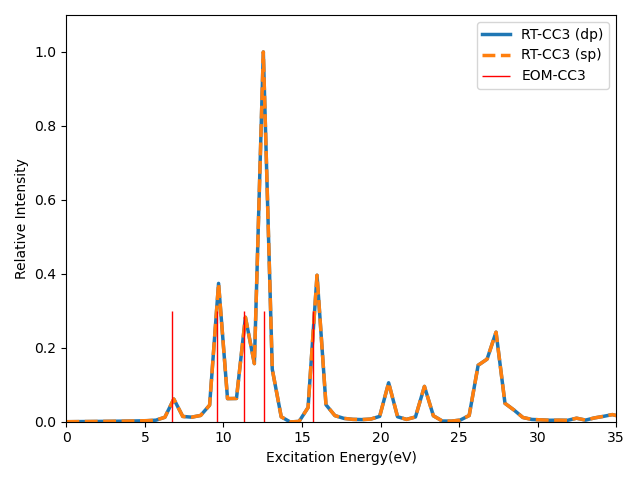
\includegraphics[angle=0, scale=0.43]{ch4/Figs/1-1.png}
    \caption{RT-CC3/cc-pVDZ linear absorption spectrum of \ch{H_{2}O} and corresponding EOM-CC3/cc-pVDZ transitions included as stick-spectra for comparison.}
    \label{fig:abs-water}
\end{figure}
To assess the stability and accuracy of the RT-CC3 implementation, we initially calculated the linear absorption spectrum using the procedure outlined in section~\ref{theory-cc3-21}. To generate a broadband spectrum, a thin Gaussian pulse was applied. The absorption spectrum was computed for both single- and double-precision arithmetics, as depicted in Fig.~\ref{fig:abs-water}. It has been demonstrated that single-precision is sufficient for calculating the absorption spectrum using RT-CCSD in our previous work.\cite{Wang2022} Similarly, in this specific test case, no significant distinction between single- and double-precision results is discernible in the RT-CC3 outcomes. For the EOM-CC3/cc-pVDZ calculation, only excitation energies are attainable from Psi4, while the corresponding oscillator strengths remain unavailable. For illustrative purposes, the `height' of the stick spectra is arbitrarily chosen to enable convenient visualization of the position of each state. However, this choice doesn't convey any information about the probability of the corresponding transition. Through this comparison, we can ascertain that the RT-CC3 method aligns with the EOM-CC3 method.

\subsubsection{Dynamic Polarizabilities and First Hyperpolarizabilities}\label{results-cc3-22}
%Fig2-RTCC3-RCW
\begin{figure}
    \centering
    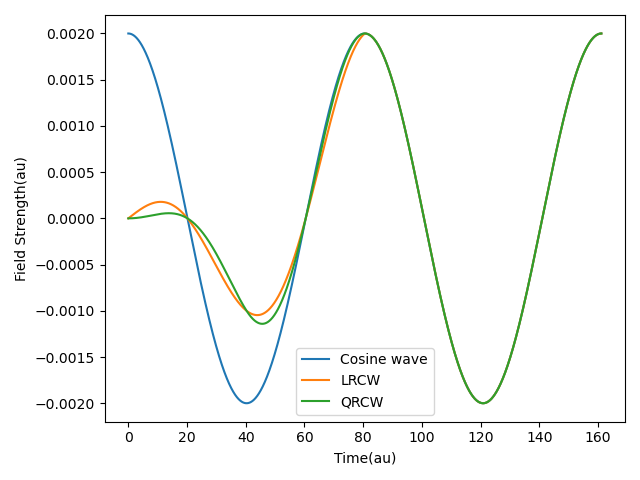
\includegraphics[angle=0, scale=0.43]{ch4/Figs/2-1.png}
    \caption{LRCW and QRCW of two optical cycles. Both of the RCWs have one ramped cycle following a cycle with a regular cosine wave. The frequency and the field strength are 0.078 au and 0.002 au, respectively.}
    \label{fig:rcw}
\end{figure}
As demonstrated in Ref.~\citenum{Ofstad2023}, the QRCW is favorable for extracting optical properties as it has a smoother switch-on compared to the LRCW or a simple oscillatory field without ramping. Fig.~\ref{fig:rcw} illustrates that both LRCW and QRCW have significantly smaller amplitudes at the initial stages of the simulation compared to the regular cosine wave. The QRCW curve exhibits a more gradual increase than the LRCW curve during the first 20 au. Here, we apply both the LRCW and the QRCW to showcase the effect of ramping.

Dynamic polarizabilities and first hyperpolarizabilities of \ch{H_{2}O} at the level of CCSD and CC3 are calculated using finite-difference methods. The simulation with the LRCW spans five ramped cycles, with the first cycle including ramping. In contrast, the simulation with the QRCW encompasses two optical cycles, with ramping applied to the first cycle. The calculations are conducted using both single-precision (sp) and double-precision (dp) arithmetics. A representative result of RT-CCSD/cc-pVDZ (dp) for \ch{H_{2}O} is depicted in Fig.~\ref{fig:pol-hyp-fit} to elucidate the procedure for obtaining polarizabilities and first hyperpolarizabilities. 

From the fitted curve of the time trajectory of the first-order dipole moment, the corresponding polarizability component can be calculated as the amplitude of the curve. As depicted in Fig.~\ref{fig:pol-hyp-fit}, the values of $\alpha_{z}$ at $\omega=0.078$ au are 7.019 au and 7.014 au, respectively, when utilizing the LRCW and QRCW. Regarding the first hyperpolarizabilities, the time trajectory of the second-order dipole moment is fitted into a cosine curve, determining the amplitude $A$ and the phase $B$, which represent the hyperpolarizabilities associated with SHG and OR, respectively. The quality of the curve fitting is assessed using the R$^{2}$ value. As shown in Fig.~\ref{fig:pol-hyp-fit}, a well-fitting curve is characterized by an R$^{2}$ value close to one, whereas a relatively inadequate fitting due to an irregular-shaped second-order dipole trajectory is indicated by an R$^{2}$ value as low as 0.89911. The summarized results are presented in Tables~\ref{tab:polar},~\ref{tab:hyp-shg} and~\ref{tab:hyp-or}.
% Fig3: RT-CC3-pol-hyp-fit
\begin{figure}
     \centering
     \begin{subfigure}{0.47\textwidth}
         \centering
         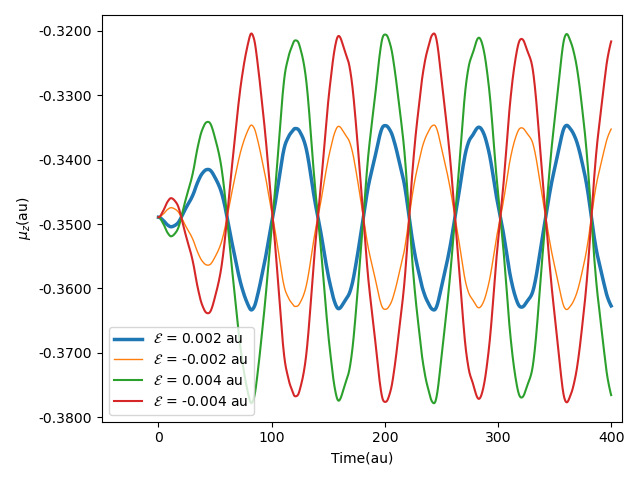
\includegraphics[width=\textwidth]{ch4/Figs/3-1.png}
     \end{subfigure}
     \hfill
     \begin{subfigure}{0.47\textwidth}
         \centering
         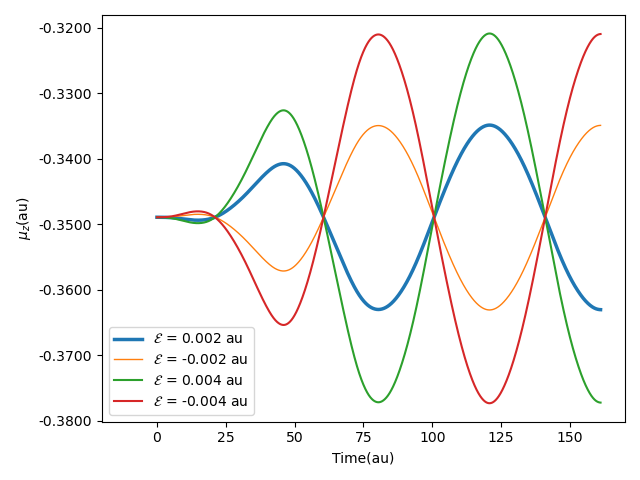
\includegraphics[width=\textwidth]{ch4/Figs/3-4.png}
     \end{subfigure}
     \vfill
     \begin{subfigure}{0.47\textwidth}
         \centering
         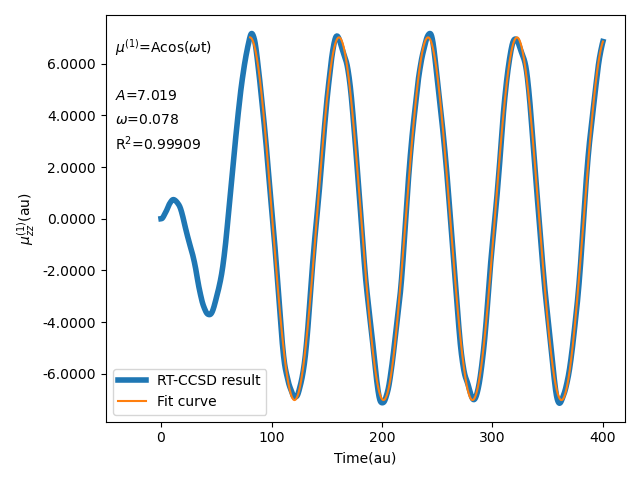
\includegraphics[width=\textwidth]{ch4/Figs/3-2.png}
     \end{subfigure}
     \hfill
     \begin{subfigure}{0.47\textwidth}
         \centering
         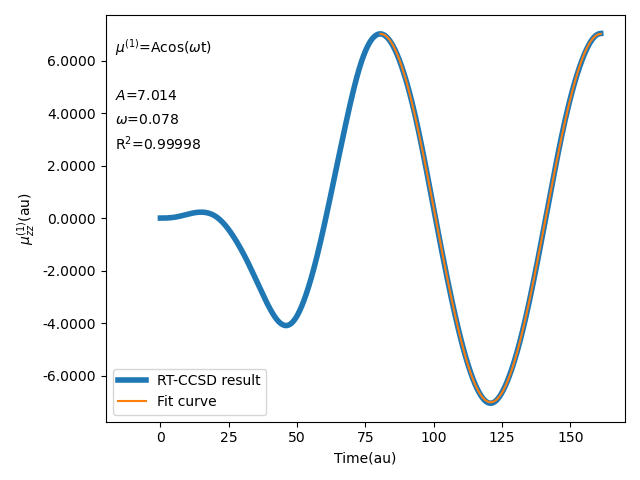
\includegraphics[width=\textwidth]{ch4/Figs/3-5.png}
     \end{subfigure}
     \vfill
     \begin{subfigure}{0.47\textwidth}
         \centering
         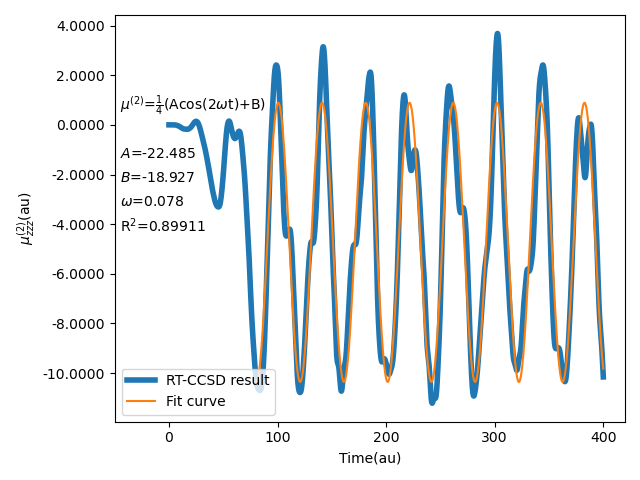
\includegraphics[width=\textwidth]{ch4/Figs/3-3.png}
     \end{subfigure}
     \hfill
     \begin{subfigure}{0.47\textwidth}
         \centering
         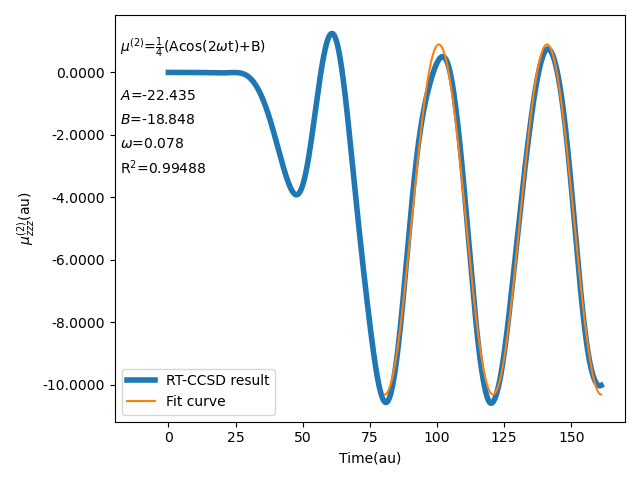
\includegraphics[width=\textwidth]{ch4/Figs/3-6.png}
     \end{subfigure}
     \caption{RT-CCSD/cc-pVDZ (dp) results of \ch{H_{2}O} obtained from four simulations with field strengths of 0.002 au, -0.002 au, 0.004 au, and -0.004 au. The left column displays the LRCW results, including the $z$ component of the induced electric dipole moment, along with the corresponding first- and second-order dipole moments. These are presented from top to bottom along with their fitted curves. The right column showcases the QRCW results.}
     \label{fig:pol-hyp-fit}
\end{figure}

To assess the performance of different simulations, three criteria are evaluated: (1) accuracy compared to linear response (LR) CC, (2) R$^{2}$ value, and (3) simulation length. A method capable of delivering accurate results from a relatively short simulation, along with a curve fitting that yields a high R$^{2}$ value, is the preferable choice. We employ the percentage error to quantify accuracy, which is calculated using the following formula:
\begin{equation}
\textrm{Percentage Error} = |\frac{x - x_{0}}{x_{0}}| \times 100\%,
\end{equation}
where $x$ is the measured value and $x_{0}$ is the reference value. 
% Table2-polarizabilities
\begin{table}
  \centering
  \caption{RT-CCSD/cc-pVDZ and RT-CC3/cc-pVDZ polarizabilities (in atomic units) of \ch{H_{2}O} at 582 nm from simulations with linear ramped continuous wave (LRCW) or quadratic ramped continuous wave (QRCW) fields. Reference values from LR-CCSD and LR-CC3 calculations using CFOUR are provided for comparison. The R$^{2}$ values, indicating the quality of curve fitting, are presented in the last three columns.}
  \begin{tabular}{c|c|ccc|ccc}
                                        & \textrm{Method} & $\alpha_{xx}$ & $\alpha_{yy}$ & $\alpha_{zz}$ 
                                          & R$^{2}_{\alpha_{xx}}$ & R$^{2}_{\alpha_{yy}}$ & R$^{2}_{\alpha_{zz}}$\\
                                          \hline
   & \textrm{LR-CCSD} & 3.182 & 10.549 & 7.017 & & &\\  
    \hline                                     
 \textrm{LRCW}  & \textrm{RT-CCSD\ (dp)} & 3.183 & 10.549 &  7.019 & 0.99980 & 0.99994 & 0.99909 \\
                           & \textrm{RT-CCSD\ (sp)} &  3.183 & 10.549 & 7.019 & 0.99980 & 0.99994 & 0.99909\\
    \cline{1-8}
  \textrm{QRCW} & \textrm{RT-CCSD\ (dp)} & 3.182 & 10.549 &  7.014 & 0.99999 & 0.99994 & 0.99998 \\
                           &\textrm{RT-CCSD\ (sp)} &  3.182 & 10.549 & 7.014 & 0.99999 & 0.99994 & 0.99998\\
    \hline\hline
   & \textrm{LR-CC3} & 3.164 & 10.581 & 7.007 & \\
    \hline
    \textrm{LRCW} &\textrm{RT-CC3\ (dp)} & 3.164 & 10.584 & 7.010 & 0.99981 & 0.99993 & 0.99908 \\
                             &\textrm{RT-CC3\ (sp)} & 3.164 & 10.584 & 7.010 & 0.99981 & 0.99993 & 0.99908 \\
    \cline{1-8}
    \textrm{QRCW} &\textrm{RT-CC3\ (dp)} & 3.165 & 10.580 & 7.004 & 0.99999 & 0.99995 & 0.99998 \\
                             &\textrm{RT-CC3\ (sp)} & 3.165 & 10.580 & 7.004 & 0.99999 & 0.99995 & 0.99998 \\
  \end{tabular}
  \label{tab:polar}
\end{table}

For polarizabilities, the single- and double-precision calculations yield identical results up to three decimal places, with the same R$^{2}$ values accurate for five decimal places. Minor discrepancy can be observed when comparing to the LRCW  and the QRCW results. In RT-CCSD simulations, the LRCW results exhibit a $0.03\%$ error in $\alpha_{xx}$ and a $0.03\%$ error in $\alpha_{zz}$ , while the QRCW results show a $0.04\%$ error in $\alpha_{zz}$. In the case of RT-CC3 simulations, the LRCW results show a $0.03\%$ error in $\alpha_{yy}$ and a $0.05\%$ error in $\alpha_{zz}$ , while the QRCW results indicate a $0.03\%$ error in $\alpha_{xx}$, a $0.01\%$ error in $\alpha_{yy}$ and a $0.05\%$ error in $\alpha_{zz}$. Both of the two ramped continuous waves yield errors well below $0.1\%$. Furthermore, the QRCW requires less simulation time compared to the LRCW and offers a slightly better curve fitting. As a result, the QRCW is the preferred choice, and this conclusion applies to both RT-CCSD and RT-CC3 simulations.
% Table3-hyperpolarizabilities (SHG)
\begin{table}
  \centering
  \caption{RT-CCSD/cc-pVDZ and RT-CC3/cc-pVDZ first hyperpolarizabilities (in atomic units) associated with second harmonic generation (SHG) of \ch{H_{2}O} at 582 nm obtained from simulations with linear ramped continuous wave (LRCW) and quadratic ramped continuous wave (QRCW) fields. Reference values from LR-CCSD calculations using CFOUR are provided. The R$^{2}$ values, reflecting the quality of curve fitting, are displayed in the last three columns.}
  \begin{tabular}{c|c|ccc|ccc}
                                        &  \textrm{Method}  & $\beta_{zxx}$ & $\beta_{zyy}$ & $\beta_{zzz}$ 
                                          & R$^{2}_{\beta_{zxx}}$ & R$^{2}_{\beta_{zyy}}$ & R$^{2}_{\beta_{zzz}}$\\
                                          \hline
    & \textrm{LR-CCSD} & -4.091 & -35.441 & -22.423 & & &\\                 
    \hline                      
     \textrm{LRCW} & \textrm{RT-CCSD\ (dp)} & -4.311 & -35.694 &  -22.485 & 0.93021 & 0.54362 & 0.89911 \\
                              & \textrm{RT-CCSD\ (sp)} & -4.298 & -35.707 & -22.482 & 0.92954 & 0.54195 & 0.89921 \\
    \hline
     \textrm{QRCW} & \textrm{RT-CCSD\ (dp)} & -4.053 & -35.469 &  -22.435 & 0.99892 & 0.97345 & 0.99488 \\
                              & \textrm{RT-CCSD\ (sp)} & -3.987 & -35.520 & -22.447 & 0.99169 & 0.97266 & 0.99480 \\
    \hline\hline
    \textrm{LRCW} & \textrm{RT-CC3\ (dp)} & -3.848 & -36.682 & -21.736 & 0.91595 & 0.67373 & 0.89616 \\
                             & \textrm{RT-CC3\ (sp)} & -3.846 & -36.749 & -22.696 & 0.92203 & 0.67353 & 0.89689 \\
      \hline
     \textrm{QRCW} & \textrm{RT-CC3\ (dp)} & -3.831 & -35.450 & -21.708 & 0.99887 & 0.97111 & 0.99476 \\
                             & \textrm{RT-CC3\ (sp)} & -3.841 & -35.444 & -21.694 & 0.99559 & 0.97180 & 0.99444 \\
  \end{tabular}
  \label{tab:hyp-shg}
\end{table}
% Table4-hyperpolarizabilities (SHG)-error
\begin{table}
  \centering
    \caption{Percentage errors of RT-CCSD/cc-pVDZ first hyperpolarizabilities (au) associated with SHG of \ch{H_{2}O} at 582 nm from calculations using LRCW and QRCW.}
  \begin{tabular}{c|c|ccc}
                                        &  \textrm{Method}  & $\beta_{zxx}$ & $\beta_{zyy}$ & $\beta_{zzz}$ \\
                                          \hline                   
     \textrm{LRCW} & \textrm{RT-CCSD\ (dp)} & 5.38\% & 0.71\% &  0.28\%  \\
                              & \textrm{RT-CCSD\ (sp)} & 5.06\% & 0.75\% & 0.26\%  \\
    \hline
     \textrm{QRCW} & \textrm{RT-CCSD\ (dp)} & 0.93\% & 0.08\% &  0.05\%  \\
                              & \textrm{RT-CCSD\ (sp)} & 2.59\% & 0.22\% & 0.11\%  \\
     \end{tabular}
      \label{tab:hyp-shg-error}
\end{table}
% Table5-hyperpolarizabilities (OR)
\begin{table}
  \centering
    \caption{RT-CCSD/cc-pVDZ and RT-CC3/cc-pVDZ first hyperpolarizabilities (in atomic units) associated with optical rectification (OR) of \ch{H_{2}O} at 582 nm obtained from simulations with linear ramped continuous wave (LRCW) and quadratic ramped continuous wave (QRCW) fields. Reference values from LR-CCSD calculations using CFOUR are provided. The R$^{2}$ values, indicating the quality of curve fitting, are displayed in the last three columns.}
  \begin{tabular}{c|c|ccc|ccc}
                                        &  \textrm{Method}  & $\beta_{zxx}$ & $\beta_{zyy}$ & $\beta_{zzz}$ 
                                          & R$^{2}_{\beta_{zxx}}$ & R$^{2}_{\beta_{zyy}}$ & R$^{2}_{\beta_{zzz}}$\\
                                          \hline
   & \textrm{LR-CCSD} & -4.488 & -30.485 & -18.830 & & &\\  
    \hline                                     
    \textrm{LRCW} & \textrm{RT-CCSD\ (dp)} & -4.532 & -30.568 &  -18.927 & 0.93021 & 0.54362 & 0.89911 \\
                              &   \textrm{RT-CCSD\ (sp)} &  -4.579 & -30.624 & -18.977 & 0.92954 & 0.54195 & 0.89921 \\
    \hline
    \textrm{QRCW} & \textrm{RT-CCSD\ (dp)} & -4.481 & -30.513 &  -18.848 & 0.99892 & 0.97345 & 0.99488 \\
                              &   \textrm{RT-CCSD\ (sp)} &  -4.445 & -30.733 & -18.918 & 0.99169 & 0.97266 & 0.99480 \\
    \hline\hline
     \textrm{LRCW} & \textrm{RT-CC3\ (dp)} & -4.272 & -30.908 & -18.300 & 0.91596 & 0.67373 & 0.89616 \\
                               &   \textrm{RT-CC3\ (sp)} & -4.331 & -30.839 & -18.159 & 0.92203 & 0.67353 & 0.89436 \\
      \hline
      \textrm{QRCW} & \textrm{RT-CC3\ (dp)} & -4.242 & -30.446 & -18.220 & 0.99887 & 0.97111 & 0.99476 \\
                               &   \textrm{RT-CC3\ (sp)} & -4.286 & -30.555 & -18.079 & 0.99559 & 0.97180 & 0.99444 \\
  \end{tabular}
  \label{tab:hyp-or}
\end{table}
% Table6-hyperpolarizabilities (OR)-error
\begin{table}
  \centering
    \caption{Percentage errors of RT-CCSD/cc-pVDZ first hyperpolarizabilities (au) associated with OR of \ch{H_{2}O} at 582 nm from calculations using LRCW and QRCW.}
  \begin{tabular}{c|c|ccc}
                                        &  \textrm{Method}  & $\beta_{zxx}$ & $\beta_{zyy}$ & $\beta_{zzz}$ \\
                                          \hline                   
     \textrm{LRCW} & \textrm{RT-CCSD\ (dp)} & 0.98\% & 0.27\% &  0.51\%  \\
                              & \textrm{RT-CCSD\ (sp)} & 2.03\% & 0.46\% & 0.78\%  \\
    \hline
     \textrm{QRCW} & \textrm{RT-CCSD\ (dp)} & 0.16\% & 0.09\% &  0.10\%  \\
                              & \textrm{RT-CCSD\ (sp)} & 0.96\% & 0.81\% & 0.47\%  \\
     \end{tabular}
  \label{tab:hyp-or-error}
\end{table}

For the first hyperpolarizabilities, we observe larger errors in RT-CCSD results compared to LR-CCSD, as well as differences between single- and double-precision results. This outcome is reasonable, considering that we are calculating a higher-order property involving induced dipole moments. It's important to note that the R$^{2}$ values in Tables~\ref{tab:hyp-shg} and~\ref{tab:hyp-or} are identical. This is because the hyperpolarizabilities associated with second harmonic generation (SHG) and optical rectification (OR) are obtained using the same curve fitting process, with the field applied in a specific direction.

Tables~\ref{tab:hyp-shg-error} and~\ref{tab:hyp-or-error} summarize the percentage errors of hyperpolarizability elements obtained from RT-CCSD calculations, compared to LR-CCSD. In Table~\ref{tab:hyp-shg-error}, the largest error of $5.38\%$ occurs in $\beta_{zxx}$ from the RT-CCSD (dp) calculation using LRCW. By switching to the QRCW, the error in $\beta_{zxx}$ is reduced by $82.71\%$, from $5.8\%$ to $0.93\%$. The percentage errors for other elements are also substantially reduced by at least $48.81\%$. Moreover, the R$^{2}$ values improve when using the QRCW, as seen in Table~\ref{tab:hyp-shg}. Notably, for $\beta_{zyy}$ where the applied field is perpendicular to the molecule's plane, a less smooth trajectory of the second-order dipole moments leads to lower R$^{2}$ values for the LRCW case. Using the QRCW recovers the quality of curve fitting, with R$^{2}$ values exceeding $0.97$.

Regarding precision arithmetic, the double-precision calculation with the LRCW outperforms the single-precision case for $\beta_{zyy}$, while showing slightly worse results for $\beta_{zxx}$ and $\beta_{zzz}$. However, for calculations using the QRCW, the single-precision arithmetic leads to larger errors for all elements. Generally, a double-precision calculation should yield more accurate and robust results because double-precision floating-point numbers are accurate up to 15 decimal places, whereas single-precision numbers are accurate only up to around 7 decimal places. In our test case, when the LRCW is used, the major error arises from the choice of external field. This can be observed from the relatively large overall error and the poor R$^{2}$ values. The difference caused by the two different precision arithmetics is not as pronounced. Neither of them produces sufficiently accurate results. However, when the QRCW is employed, the percentage error is significantly reduced due to the more gradual switch-on of the field, regardless of the chosen precision arithmetics. Consequently, the lower precision arithmetic becomes the primary factor contributing to the resulting error. This is evident in the last two rows of Table~\ref{tab:hyp-shg-error}, where errors in single-precision calculations are 120\% to 178\% larger than those in double-precision calculations.

A similar analysis applies to the results of hyperpolarizabilities associated with OR, as shown in Tables~\ref{tab:hyp-or} and~\ref{tab:hyp-or-error}. In this case, the percentage errors originating from the LRCW are not as significant as those observed in the case of hyperpolarizabilities associated with SHG. Results from the double-precision calculations are consistently more accurate than the single-precision results. Furthermore, the QRCW continues to significantly enhance accuracy for each element, consistent with the trends observed for hyperpolarizabilities associated with SHG.

In the context of RT-CC3 calculations, even though reference values are unavailable for direct comparison, the impact of replacing the LRCW with the QRCW is evident from the substantial increase in R$^{2}$ values. The excellent R$^{2}$ values observed in RT-CC3 calculations involving the QRCW further reinforce the notion that our implementation serves as a viable tool for calculating dynamic polarizability and first hyperpolarizabilities at the CC3 level, given the limitations of available alternatives.

The results presented above demonstrate the capability of the RT-CC3 method for calculating polarizabilities and first hyperpolarizabilities. Given the approximated orbital relaxation with singles in CC3, it is worthwhile to explore a comparison to orbital-optimized coupled cluster (OCC) methods. In time-dependent OCC methods, the singles are replaced by orbital rotations. As an example, Kristiansen et al. implemented real-time (RT) time-dependent orbital-optimized M\o{}ller-Plesset (TDOMP2) theory, which serves as a second-order approximation to the time-dependent orbital-optimized coupled cluster doubles (TDOCCD) method.\cite{Kristiansen2022} TDOMP2 is further compared to RT-CC2, which is a second-order approximation to RT-CCSD. The explicit orbital optimization is proven to be significant for polarizabilities and hyperpolarizabilities, with TDOMP2 outperforming RT-CC2. However, this optimization does not play a critical role in the absorption spectrum, as both methods yield nearly identical spectra.

In addition to the TDOMP2 method, Kristiansen et al. also developed the time-dependent nonorthogonal OCCD (TDNOCCD) method, where the orbital rotation is non-unitary. To assess the performance of RT-CC3 and TDNOCCD for polarizabilities, several ten-electron systems are investigated using double-precision calculations to mitigate errors stemming from low-precision arithmetic. Table~\ref{tab:noccd} presents the TDNOCCD results provided by Kristiansen and compares them with our RT-CC3 results. Reference values include FCI values and LR results, with RT-CCSD results included for comparison. FCI and LR-CC3 values for \ch{Ne} and \ch{HF} are obtained from Ref.~\citenum{Larsen1999}. LR-CC3 values for other molecules are computed using CFOUR. All RT simulations employ the QRCW as the applied field, with one ramped cycle followed by a regular cycle.

For \ch{Ne}, RT-CC3 exhibits good agreement with LR-CC3 and FCI, with errors as large as $0.67\%$ for frequencies ranging from 0.1 au to 0.3 au. However, a notable deviation from LR-CC3/FCI results becomes apparent at a frequency of 0.4 au, which is closer to the resonance at 0.613 au. The accuracy of the result at $\omega=0.5\ au$ is expected to be even lower, as indicated by the comparison between LR-CCSD and RT-CCSD. Surprisingly, the result at $\omega=0.5\ au$ is closer to the reference value. To assess the quality of curve fitting, R$^{2}$ values are compared for different frequencies. The R$^{2}$ values for $\omega=0.3\ au$, $\omega=0.4\ au$, and $\omega=0.5\ au$ are 0.99999, 0.99317, and 0.98147, respectively. These values decrease with higher frequencies. While the result at $\omega=0.5\ au$ is "accurate," it is somewhat less reliable than the results for lower frequencies.

A similar trend is observed for \ch{HF}. RT-CC3 regains accuracy compared to LR-CC3 and FCI at frequencies of 0.1 au and 0.2 au. At a frequency of 0.3 au, which is quite close to the resonance at 0.383 au, the accuracy decreases, resulting in percentage errors of $8.13\%$ and $1.96\%$ for $\alpha_{yy}$ and $\alpha_{zz}$, respectively. Corresponding R$^{2}$ values are 0.97621 and 0.97826, respectively. The error in $\alpha_{zz}$ is slightly smaller than in $\alpha_{yy}$ due to the H-F bond aligning with the z-axis, contributing a nonzero static dipole component, $(\mu_{0})_{z}$. The observed pattern in CC3 results aligns with that in CCSD results.

For \ch{H_{2}O}, selected frequencies are all below the resonance at 0.277 au. RT-CC3 values consistently align with LR-CC3, with only a $0.11\%$ error observed in $\alpha_{zz}$ at $\omega=0.1\ au$. In the case of \ch{NH_{3}}, RT-CC3 results match LR-CC3 values for all frequencies chosen, which are all below the resonance at 0.236 au. The exception is $\alpha_{zz}$ at $\omega=0.1\ au$, where a $0.87\%$ error occurs. This discrepancy contrasts with the agreement between LR-CCSD and RT-CCSD at the same frequency. Notably, the $C_{3}$ axis is aligned with the y-axis, and this significant error is absent in $\alpha_{yy}$.

A similar divergence is seen in the results for \ch{CH_{4}} at the frequency of 0.2 au, whereas the resonance occurs at 0.38 au. RT-CC3 results show a $1.02\%$ deviation from LR-CC3, compared to a mere $0.15\%$ discrepancy in the CCSD case. The corresponding R$^{2}$ values for these two less accurate results, $\alpha_{zz}$ of \ch{NH_{3}} and the polarizability of \ch{CH_{4}}, are 0.99823 and 0.99574, respectively. These values are smaller than those of the other polarizability values, which are all above 0.9999.

To further explore the differences between RT-CCSD and RT-CC3 in these cases, we calculated two additional LR-CCSD/LR-CC3 polarizabilities at different frequencies and performed polynomial regression with five data points. This analysis reveals the relationship between increasing polarizabilities and frequency. In addition to the values listed in Table~\ref{tab:noccd}, $\alpha_{zz}$ of \ch{NH_{3}} is calculated at a frequency of 0.025 au, yielding LR-CC3 and LR-CCSD results of 14.88 au and 14.90 au, respectively. At a frequency of 0.085 au, $\alpha_{zz}$ values are 15.72 au and 15.74 au for LR-CC3 and LR-CCSD, respectively. Two more frequencies, 0.0428 au and 0.15 au, are selected for \ch{CH_{4}}. RT-CC3 and RT-CCSD results at $\omega=0.0428\ au$ are 16.89 au and 16.91 au, respectively. At $\omega=0.15\ au$, the corresponding results are 18.20 au and 18.21 au, respectively.

As shown in Fig.~\ref{fig:polar-polyfit}, polynomial regression closely aligns with data points for all four data sets, with R$^{2}$ values exceeding 0.9999. Moreover, the coefficients of $\omega^{3}$ from LR-CC3 data are larger than those from LR-CCSD data for both \ch{NH_{3}} and \ch{CH_{4}}. The polynomial regression results suggest that CC3 polarizabilities increase slightly faster with frequency compared to CCSD polarizabilities. The impact of frequency moving towards the resonance on polarizability results becomes evident earlier in the frequency range for CC3 compared to CCSD in these test cases, potentially explaining the disagreement observed for polarizability values of \ch{NH_{3}} and \ch{CH_{4}}.

The impact of orbital optimization is explored by comparing TDNOCCD with RT-CCSD and higher levels of theory. As previously mentioned, TDNOCCD differs from RT-CCSD by substituting singles with a non-unitary orbital rotation, where the rotation parameter is time-dependent. OCC-type methods have demonstrated advantages in multi-electron dynamics, chemical bond breaking, response theory, and more.\cite{Pedersen2001, Kohn2005, Sato2018, Pathak2022} Explicit orbital optimization also enhances the stability of real-time simulations when systems are subjected to strong external fields, and the ground state no longer dominates.\cite{Kristiansen2020}

In our test cases, TDNOCCD is initially compared to RT-CCSD by assessing its differences from LR-CCSD. The data presented in Table~\ref{tab:noccd} indicate that TDNOCCD results exhibit relative differences ranging from $0.89\%$ to $7.09\%$, with an average difference of $2.98\%$ across all frequencies and molecules, compared to LR-CCSD. The most significant difference arises from the polarizability of \ch{Ne} at $\omega=0.5\ au$. However, this TDNOCCD result is actually closer to LR-CCSD than RT-CCSD for this specific value. Unlike the RT methods, the frequency dependence of relative differences in TDNOCCD is not as pronounced. It is evident that substantial differences are present not only in high-frequency results but also in low-frequency outcomes, which are distant from resonances. The primary factor contributing to this divergence between TDNOCCD and RT-CCSD, in comparison with LR-CCSD, is the orbital optimization.

Next, TDNOCCD results are compared to LR-CC3 and RT-CC3. Except for a few cases (e.g., \ch{Ne} at $\omega=0.4\ au$ and $0.5\ au$, \ch{HF} at $\omega=0.3\ au$, \ch{NH_{3}} at $\omega=0.1\ au$, and \ch{CH_{4}} at $\omega=0.2\ au$), RT-CC3 results match LR-CC3. However, TDNOCCD deviates from LR-CC3/RT-CC3 by at least $1.03\%$ and up to $3.41\%$, with an average divergence of $2.14\%$. As these polarizability results are unaffected by proximity to resonances, the divergence stems from distinct treatments of orbital optimization and the inclusion/exclusion of triples.

In cases where RT-CC3 exhibits significant percentage errors compared to LR-CC3, the difference between TDNOCCD and LR-CC3 may be larger or smaller than the difference between RT-CC3 and LR-CC3, depending on the RT-CC3 error. When RT-CC3 overestimates polarizability of \ch{Ne} ($\omega=0.4\ au$) and $\alpha_{zz}$ of \ch{HF} ($\omega=0.3\ au$) by $10.54\%$ and $8.13\%$, respectively, TDNOCCD yields smaller values due to orbital optimization, making it closer to LR-CC3. It ultimately underestimates these polarizability values by $2.71\%$ and $0.99\%$, respectively. The orbital-optimization effect mitigates the error and even leads to overcorrection in RT-CC3. However, when RT-CC3 underestimates polarizabilities, the even smaller values from TDNOCCD result in a larger difference from LR-CC3.
% Fig4: polyfit-polar
\begin{figure}
     \centering
     \begin{subfigure}{0.495\textwidth}
         \centering
         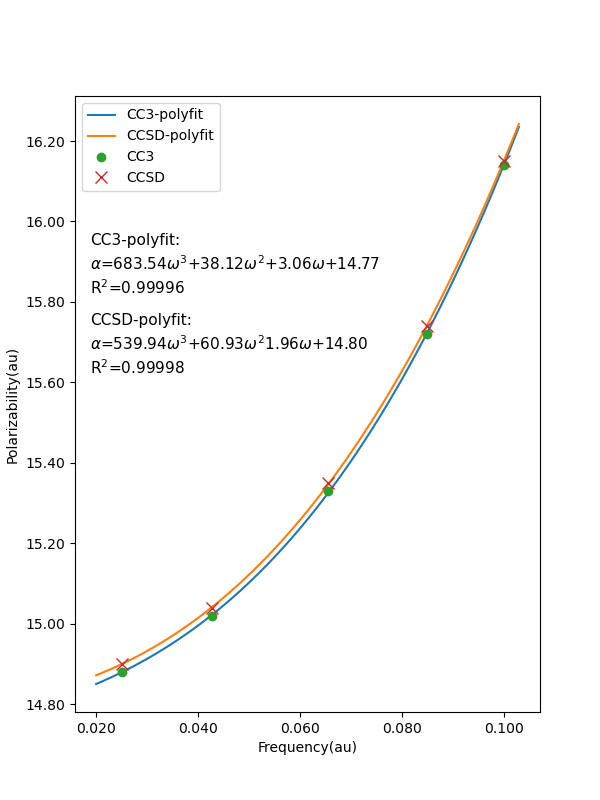
\includegraphics[width=\textwidth]{ch4/Figs/4-1.png}
     \end{subfigure}
     \hfill
     \begin{subfigure}{0.495\textwidth}
         \centering
         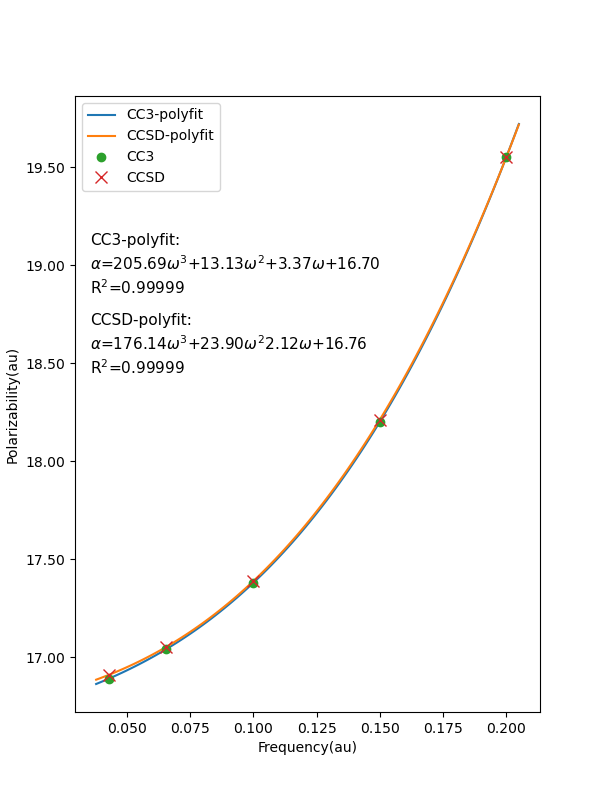
\includegraphics[width=\textwidth]{ch4/Figs/4-2.png}
     \end{subfigure}
     \caption{Variation of $\alpha_{zz}$ values for \ch{NH_{3}} (left) and polarizabilities for \ch{CH_{4}} (right) in relation to frequency, calculated using CC3 and CCSD methods. Polynomial regression curves are depicted, along with the resulting functions and R$^{2}$ values as annotations on the figures.}
     \label{fig:polar-polyfit}
\end{figure}
% Table5-RTCC3-vs-TDNOCCD
\begin{table}
\centering
\caption{Polarizabilities (in atomic units) of \ch{Ne}, \ch{HF}, \ch{H2O}, \ch{NH3} and \ch{CH4}.}
\begin{tabular}{l l r r r r r r r r r}
\hline
\hline
\ch{Ne}&$\omega\,(\text{a.u.})$ & $0.1$ & $0.2$ & $0.3$ & $0.4$ & $0.5$ \\
\hline
&FCI        &   $2.70$ & $2.79$ & $2.97$ & $3.31$ & $4.09$  \\
&LR-CC3      &   $2.71$ & $2.80$ & $2.98$ & $3.32$ & $4.10$  \\
&RT-CC3      &   $2.71$ & $2.80$ & $2.99$ & $3.67$ & $4.11$  \\
&LR-CCSD     &   $2.74$ & $2.83$ & $3.01$ & $3.38$ & $4.23$  \\		 
&RT-CCSD     &   $2.74$ & $2.83$ & $3.03$ & $3.49$ & $4.76$  \\
&TDNOCCD    &   $2.66$ & $2.75$ & $2.92$ & $3.41$ & $3.93$   \\
\hline
\ch{HF}&$\omega\,(\text{a.u.})$        & \multicolumn{2}{c}{$0.1$}&  \multicolumn{2}{c}{$0.2$} & \multicolumn{2}{c}{$0.3$}            \\ 
&                      & $\alpha_{yy}$   & $\alpha_{zz}$ & $\alpha_{yy}$   & $\alpha_{zz}$ & $\alpha_{yy}$   & $\alpha_{zz}$ \\
\hline
&FCI      & $4.39$ & $6.33$ & $4.76$ & $6.74$ & $6.00$ & $7.63$ \\
&LR-CC3    & $4.39$ & $6.34$ & $4.77$ & $6.76$ & $6.03$ & $7.64$ \\ 
&RT-CC3    & $4.39$ & $6.34$ & $4.77$ & $6.76$ & $6.52$ & $7.49$ \\ 
&LR-CCSD   &     $4.44$      &   $6.41$  &     $4.83$      &  $6.83$ &     $6.19$      &   $7.73$          \\
&RT-CCSD   & $4.45$ & $6.41$ & $4.84$ & $6.83$ & $6.72$ & $7.84$\\
&TDNOCCD  & $4.30$ & $6.21$ & $4.63$ & $6.60$ & $6.09$ & $7.35$ \\
\hline
\ch{H2O} & $\omega\,(\text{a.u.})$ & \multicolumn{3}{c}{$0.0428$} & \multicolumn{3}{c}{$0.0656$} & \multicolumn{3}{c}{$0.1$} \\
&                      & $\alpha_{xx}$          & $\alpha_{yy}$   & $\alpha_{zz}$ & $\alpha_{xx}$  & $\alpha_{yy}$   & $\alpha_{zz}$ & $\alpha_{xx}$  & $\alpha_{yy}$   & $\alpha_{zz}$ \\
\hline 
&LR-CC3   &     $8.72$    &     $9.86$       &   $9.04$      &     $8.83$    &     $9.92$       &   $9.12$      &     $9.10$    &     $10.06$      &   $9.30$\\
&RT-CC3   &     $8.72$    &     $9.86$       &   $9.04$      &     $8.83$    &     $9.92$      &   $9.12$      &     $9.10$    &     $10.06$      &   $9.31$\\
&LR-CCSD   &     $8.78$    &     $9.93$       &   $9.11$      &     $8.89$    &     $9.99$       &   $9.19$      &     $9.18$    &     $10.14$      &   $9.37$\\
&RT-CCSD   &     $8.78$    &     $9.93$       &   $9.11$      &     $8.90$    &     $10.00$      &   $9.19$      &     $9.19$    &     $10.14$      &   $9.37$\\
&TDNOCCD  &     $8.45$       &   $9.67$               & $8.84$              &  $8.55$             &  $9.73$                &   $8.90$            &     $8.79$    &     $9.86$       &   $9.07$\\
\hline
\ch{NH3} & $\omega\,(\text{a.u.})$        & \multicolumn{2}{c}{$0.0428$} & \multicolumn{2}{c}{$0.0656$} & \multicolumn{2}{c}{$0.1$} \\
&        & $\alpha_{yy}$   & $\alpha_{zz}$ & $\alpha_{yy}$& $\alpha_{zz}$ & $\alpha_{yy}$& $\alpha_{zz}$ \\
\hline 
&LR-CC3   &      $13.05$    &    $15.02$    & $13.15$      &   $15.33$     & $13.39$      & $16.14$       \\
&RT-CC3   &      $13.05$    &    $15.02$    & $13.15$      &   $15.33$     & $13.38$      & $16.00$       \\
&LR-CCSD   &      $13.10$    &    $15.04$    & $13.20$      &   $15.35$     & $13.44$      & $16.15$       \\
&RT-CCSD   &      $13.10$    &    $15.05$    & $13.20$      &   $15.36$     & $13.45$      & $16.15$       \\
&TDNOCCD  &      $12.85$    &    $14.57$    & $12.94$      &   $14.84$     & $13.17$      & $15.51$       \\
\hline
\ch{CH4}&$\omega\,(\text{a.u.})$ & $0.0656$ & $0.1$ & $0.2$\\
\hline
&LR-CC3   & $17.04$ & $17.38$ & $19.55$ \\ 
&RT-CC3   & $17.04$ & $17.37$ & $19.35$ \\
&LR-CCSD   & $17.05$ & $17.39$ & $19.55$ \\ 
&RT-CCSD   & $17.05$ & $17.39$ & $19.58$ \\
&TDNOCCD  & $16.86$ & $17.19$ & $19.22$ \\
\hline
\hline
\end{tabular}
\label{tab:noccd}
\end{table}

% G' tensor 
\subsubsection{$G'$ tensor}\label{results-cc3-23}
% Fig5: RT-CC3-G' tensor
\begin{figure}
     \centering
     \begin{subfigure}{0.47\textwidth}
         \centering
         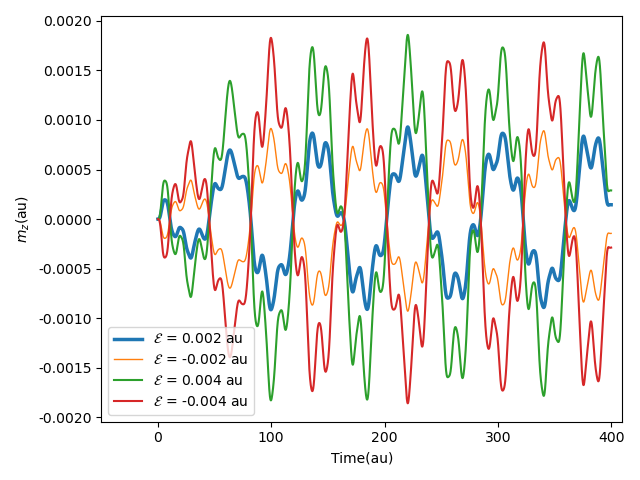
\includegraphics[width=\textwidth]{ch4/Figs/5-1.png}
     \end{subfigure}
     \hfill
     \begin{subfigure}{0.47\textwidth}
         \centering
         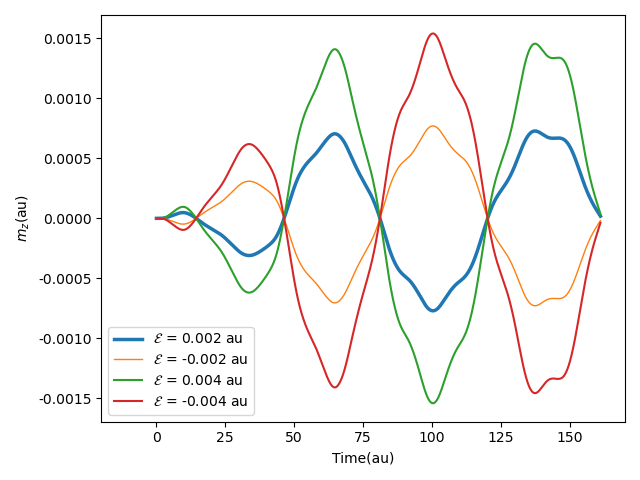
\includegraphics[width=\textwidth]{ch4/Figs/5-3.png}
     \end{subfigure}
     \vfill
     \begin{subfigure}{0.47\textwidth}
         \centering
         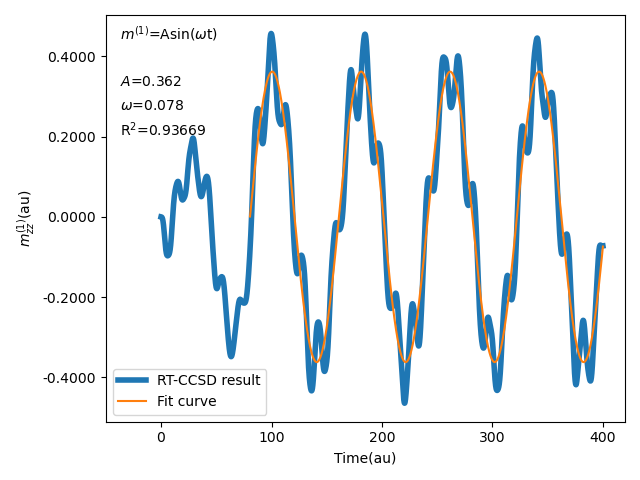
\includegraphics[width=\textwidth]{ch4/Figs/5-2.png}
     \end{subfigure}
     \hfill
     \begin{subfigure}{0.47\textwidth}
         \centering
         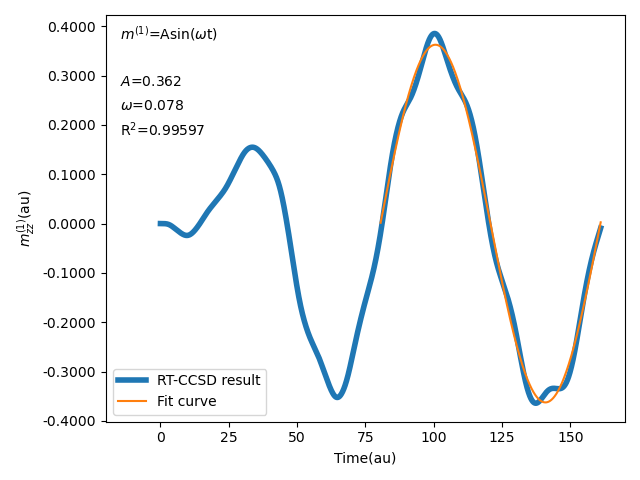
\includegraphics[width=\textwidth]{ch4/Figs/5-4.png}
     \end{subfigure}
     \caption{RT-CCSD/cc-pVDZ (dp) results of \ch{H_{2}} dimer obtained from four simulations with field strengths of 0.002 au, -0.002 au, 0.004 au, and -0.004 au. The left column displays the LRCW results, including the $z$ component of the induced magnetic dipole moment and the corresponding first-order dipole moments with their fitted curve. The right column presents the QRCW results.}
     \label{fig:g-fit}
\end{figure}
With our RT-CC implementation, we calculate the $G'$ tensor of the \ch{H_{2}} dimer using RT-CCSD and RT-CC3, both in single- and double-precision arithmetics. We employ both the LRCW and the QRCW for comparison purposes. As illustrated in Fig.~\ref{fig:g-fit}, we utilize the induced magnetic dipole moments from applied fields of varying strengths to compute the first-order magnetic dipole moments through the finite difference method, similar to the procedure for calculating polarizabilities. In this case, $G'_{zz}$ can be obtained from the magnetic dipole moment induced by the field applied in the $z$ direction, with its value represented by the amplitude of the fitted curve.

As per Table~\ref{tab:g-ccsd}, no distinction is observed between single- and double-precision results in the RT-CCSD calculations. The $G'$ tensor elements exhibit identical values for both the LRCW and the QRCW cases, with the distinction lying solely in the R$^{2}$ values. Notably, the QRCW significantly enhances curve fitting quality, aligning with the conclusion drawn in section~\ref{results-cc3-22}. Upon examining the example results in Fig.~\ref{fig:g-fit}, it is evident that the induced magnetic dipole moment curves are less smooth compared to the induced electric dipole moment curves discussed in the previous section. Particularly in the LRCW instance, a curvilinear trajectory of the dipole is observed. Although this irregular shape remains approximately periodic, it adversely affects curve fitting. A minor distortion is observed in the QRCW example, which has a lesser impact on curve fitting. Table~\ref{tab:g-cc3} presents the RT-CC3 results. Analogous to RT-CCSD, the disparities between single- and double-precision results are inconsequential. The QRCW enhances overall R$^{2}$ values and provides more dependable outcomes. Hence, the RT-CC3 method proves to be a viable approach for computing the $G'$ tensor and subsequently optical rotation.
% Table6-G' tensor
\begin{table}
  \centering
    \caption{RT-CCSD/cc-pVDZ $G'$ tensor elements (in atomic units) of H$_{2}$ dimer at 582 nm obtained using single- and double-precision computations, with linear ramped continuous wave (LRCW) and quadratic ramped continuous wave (QRCW) fields. The R$^{2}$ values, indicating the quality of curve fitting, are displayed in the last three columns.}
  \begin{tabular}{c|c|c|ccc}
                                          &  $G'$ & \textrm{RT-CCSD(dp)} & R$^{2}_{x}$(dp) & R$^{2}_{y}$(dp)& R$^{2}_{z}$(dp)\\
                                          \hline
                \textrm{LRCW} & ($G'_{xx}$, $G'_{yx}$, $G'_{zx}$) & (-0.387, -0.097, 0.000) &   0.93726 & 0.93911 & 0 \\
                                          & ($G'_{xy}$, $G'_{yy}$, $G'_{zy}$) & ( 0.058,  0.013, 0.000) &   0.88177 & 0.86203 & 0 \\
                                          & ($G'_{xz}$, $G'_{yz}$, $G'_{zz}$) & ( 0.000,  0.000, 0.362) &   0 & 0 & 0.93669 \\   
                \hline
                                           &  $G'$ & \textrm{RT-CCSD(sp)} & R$^{2}_{x}$(sp) & R$^{2}_{y}$(sp)& R$^{2}_{z}$(sp)\\
                                          \hline
                \textrm{LRCW} & ($G'_{xx}$, $G'_{yx}$, $G'_{zx}$) & (-0.387, -0.097, 0.000) &   0.93727 & 0.93911 & 0 \\
                                          & ($G'_{xy}$, $G'_{yy}$, $G'_{zy}$) & ( 0.058,  0.013, 0.000) &   0.88179 & 0.86205 & 0 \\
                                          & ($G'_{xz}$, $G'_{yz}$, $G'_{zz}$) & ( 0.000,  0.000, 0.362) &   0 & 0 & 0.93669 \\  
                 \hline
                                            &  $G'$ & \textrm{RT-CCSD(dp)} & R$^{2}_{x}$(dp) & R$^{2}_{y}$(dp)& R$^{2}_{z}$(dp)\\
                                          \hline
                \textrm{QRCW} & ($G'_{xx}$, $G'_{yx}$, $G'_{zx}$) & (-0.387, -0.097, 0.000) &   0.99956 & 0.99956 & 0 \\
                                          & ($G'_{xy}$, $G'_{yy}$, $G'_{zy}$) & ( 0.058,  0.013, 0.000) &   0.99915 & 0.99896 & 0 \\
                                          & ($G'_{xz}$, $G'_{yz}$, $G'_{zz}$) & ( 0.000,  0.000, 0.362) &   0 & 0 & 0.99597 \\  
                 \hline
                                            &  $G'$ & \textrm{RT-CCSD(sp)} & R$^{2}_{x}$(sp) & R$^{2}_{y}$(sp)& R$^{2}_{z}$(sp)\\
                                          \hline
                \textrm{QRCW} & ($G'_{xx}$, $G'_{yx}$, $G'_{zx}$) & (-0.387, -0.097, 0.000) &   0.99956 & 0.99956 & 0 \\
                                          & ($G'_{xy}$, $G'_{yy}$, $G'_{zy}$) & ( 0.058,  0.013, 0.000) &   0.99915 & 0.99896 & 0 \\
                                          & ($G'_{xz}$, $G'_{yz}$, $G'_{zz}$) & ( 0.000,  0.000, 0.362) &   0 & 0  & 0 .99597\\  
                
   \end{tabular}
  \label{tab:g-ccsd}
\end{table}
% Table7-G' tensor
\begin{table}
  \centering
    \caption{RT-CC3/cc-pVDZ $G'$ tensor elements (in atomic units) of H$_{2}$ dimer at 582 nm obtained using single- and double-precision computations, with linear ramped continuous wave (LRCW) and quadratic ramped continuous wave (QRCW) fields. The R$^{2}$ values, indicating the quality of curve fitting, are displayed in the last three columns.}
  \begin{tabular}{c|c|c|ccc}
                                          &  $G'$ & \textrm{RT-CC3(dp)} & R$^{2}_{x}$(dp) & R$^{2}_{y}$(dp)& R$^{2}_{z}$(dp)\\
                                          \hline
                \textrm{LRCW} & ($G'_{xx}$, $G'_{yx}$, $G'_{zx}$) & (-0.388, -0.097, 0.000) &   0.93805 & 0.93987 & 0 \\
                                          & ($G'_{xy}$, $G'_{yy}$, $G'_{zy}$) & ( 0.058,  0.013, 0.000) &   0.87896 & 0.85971 & 0\\
                                          & ($G'_{xz}$, $G'_{yz}$, $G'_{zz}$) & ( 0.000,  0.000, 0.363) &   0 & 0 & 0.93589 \\   
                \hline
                                           &  $G'$ & \textrm{RT-CC3(sp)} & R$^{2}_{x}$(sp) & R$^{2}_{y}$(sp)& R$^{2}_{z}$(sp)\\
                                          \hline
                \textrm{LRCW} & ($G'_{xx}$, $G'_{yx}$, $G'_{zx}$) & (-0.388, -0.097, 0.000) &   0.93805 & 0.93987 & 0 \\
                                          & ($G'_{xy}$, $G'_{yy}$, $G'_{zy}$) & ( 0.058,  0.013, 0.000) &   0.87896 & 0.85971 & 0 \\
                                          & ($G'_{xz}$, $G'_{yz}$, $G'_{zz}$) & ( 0.000,  0.000, 0.363) &   0 & 0 & 0.93588 \\  
                 \hline
                                            &  $G'$ & \textrm{RT-CC3(dp)} & R$^{2}_{x}$(dp) & R$^{2}_{y}$(dp)& R$^{2}_{z}$(dp)\\
                                          \hline
                \textrm{QRCW} & ($G'_{xx}$, $G'_{yx}$, $G'_{zx}$) & (-0.387, -0.097, 0.000) &   0.99955 & 0.99955 & 0 \\
                                          & ($G'_{xy}$, $G'_{yy}$, $G'_{zy}$) & ( 0.058,  0.013, 0.000) &   0.99911 & 0.99891 & 0 \\
                                          & ($G'_{xz}$, $G'_{yz}$, $G'_{zz}$) & ( 0.000,  0.000, 0.362) &   0 & 0 & 0.99602 \\  
                 \hline
                                            &  $G'$ & \textrm{RT-CC3(sp)} & R$^{2}_{x}$(sp) & R$^{2}_{y}$(sp)& R$^{2}_{z}$(sp)\\
                                          \hline
                \textrm{QRCW} & ($G'_{xx}$, $G'_{yx}$, $G'_{zx}$) & (-0.387, -0.097, 0.000) &   0.99955 & 0.99955 & 0 \\
                                          & ($G'_{xy}$, $G'_{yy}$, $G'_{zy}$) & ( 0.058,  0.013, 0.000) &  0.99911 & 0.99891 & 0 \\
                                          & ($G'_{xz}$, $G'_{yz}$, $G'_{zz}$) & ( 0.000,  0.000, 0.362) &   0 & 0 & 0.99602 \\  
                
   \end{tabular}
  \label{tab:g-cc3}
\end{table}

\subsection{Electron dynamics}\label{results-cc3-3}

In this section, we delve into the electron dynamics including the Rabi oscillation and the population of excited states within the RT-CC framework. We employ \ch{H_{2}}, \ch{LiH}, and \ch{C_{2}H_{4}} as our test cases. Our examination involves the effects of both the frequency and intensity of the external field. Furthermore, we investigate the stability and viability of the RT method, particularly in scenarios where the ground state is substantially depopulated. To validate our real-time implementation, we exclusively utilize the RT-CCSD method in double-precision. Employing a higher level of theory would be superfluous for the current objectives. Nevertheless, it's worth noting that the formalism employed for the RT-CCSD (dp) simulations can be seamlessly extended to RT-CC3 or single-precision calculations if necessitated.

\subsubsection{Rabi oscillation} \label{results-cc3-31}
%% H2-rabi
\subsubsubsection{\ch{H_{2}}} \label{results-cc3-311}
% Fig6: H2-abs
\begin{figure}
   \centering
   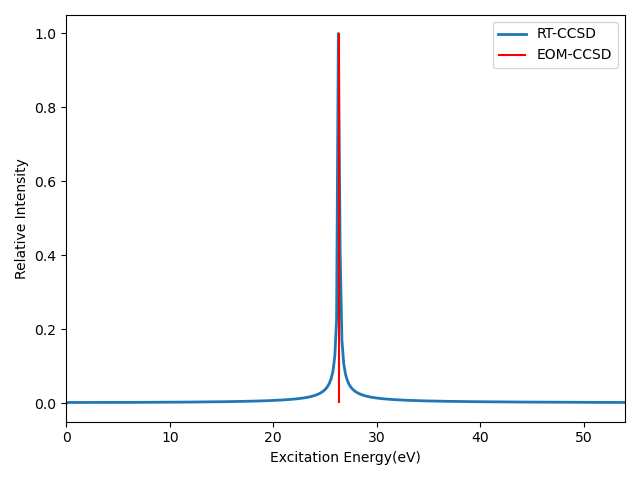
\includegraphics[angle=0, scale=0.45]{ch4/Figs/6-1.png}
   \label{fig:sp-monomer}
   \caption{RT-CCSD/STO-3G linear absorption spectrum of \ch{H_{2}} and corresponding EOM-CCSD/STO-3G transitions included as stick-spectra for comparison.}
     \label{fig:h2-abs}
\end{figure}
As a simple system comprising only two electrons, $H_{2}$ serves as an ideal molecule for testing the simulation of Rabi oscillations. We opt for a minimal basis set to eliminate complexities arising from multi-excited states. To initiate the excitation of one electron from the ground state to the excited state, we apply an oscillatory field to the system at a frequency of 0.976 au (equivalent to 26.56 eV). This frequency is determined through an EOM-CCSD/STO-3G calculation and is linked to the excitation energy of the $\sigma$-$\sigma^{*}$ transition, which is also visible in the spectrum depicted in Fig.~\ref{fig:h2-abs}. In this case, we apply the field for 500 au while varying the field strengths to observe the Rabi oscillation between the ground state S$_{0}$ and the singly-excited state S$_{1}$.

To characterize the patterns shown in Fig.~\ref{fig:h2-rabi}, we begin by examining the curves of the autocorrelation functions. It is evident that $|A(t_{0}, t)|^{2}$ oscillates between 0 and 1 for both cases. Furthermore, the Rabi frequency when the field strength is 0.0890 au (top right) is twice that of the case when the field strength is 0.0445 au (top left), which is consistent with the behavior of an ideal Rabi oscillation, where the Rabi frequency is proportional to the field strength of the driving field. Additionally, the relationship between the oscillation of the ground state population and the oscillation of the induced dipole is characteristic of Rabi oscillations. When S$_{0}$ and S$_{1}$ are equally populated, the amplitude of the dipole oscillation reaches its maximum. Conversely, when either S$_{0}$ or S$_{1}$ is fully populated, the amplitude of the dipole oscillation reaches its minimum. By observing the left and right columns of Fig.~\ref{fig:h2-rabi} respectively, it becomes apparent that the maximum amplitude in the dipole trajectory occurs when $|A(t_{0}, t)|^{2}=0.5$, and the minimum amplitude of the dipole coincides with the minima of $|A(t_{0}, t)|^{2}$ at zero or reaches the maxima at one. As demonstrated in the results, our RT-CCSD formalism successfully simulates the Rabi oscillation of \ch{H_{2}}.
% Fig7: H2-Rabi
\begin{figure}
     \centering
     \begin{subfigure}{0.47\textwidth}
         \centering
         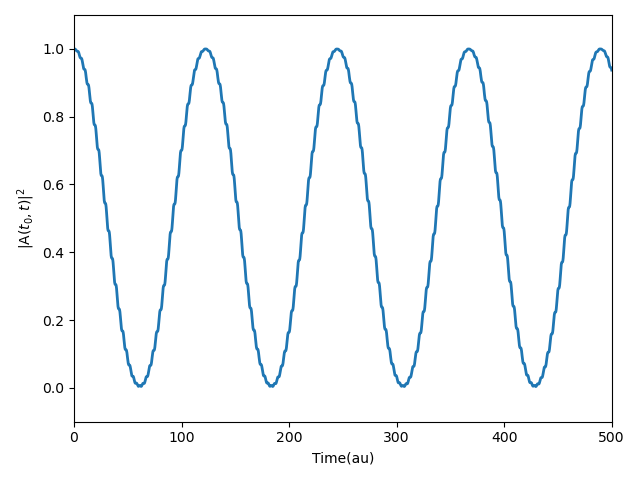
\includegraphics[width=\textwidth]{ch4/Figs/7-1.png}
     \end{subfigure}
     \hfill
     \begin{subfigure}{0.47\textwidth}
         \centering
         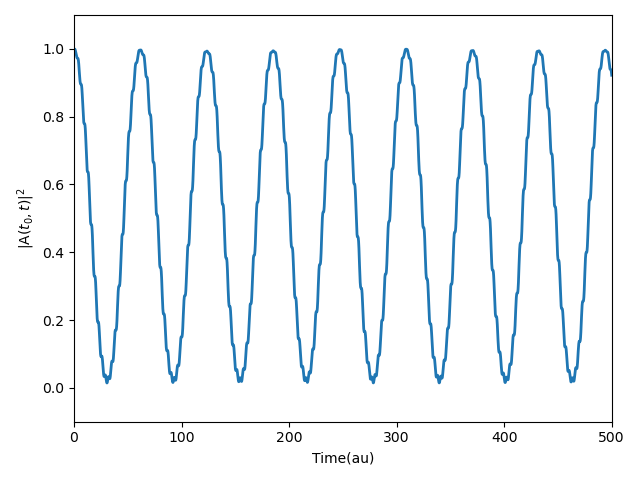
\includegraphics[width=\textwidth]{ch4/Figs/7-3.png}
      \end{subfigure}
       \vfill
     \begin{subfigure}{0.47\textwidth}
         \centering
         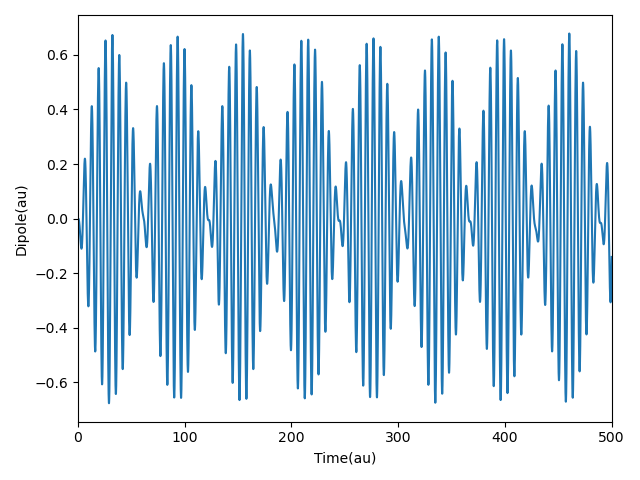
\includegraphics[width=\textwidth]{ch4/Figs/7-2.png}
     \end{subfigure}
     \hfill
     \begin{subfigure}{0.47\textwidth}
         \centering
         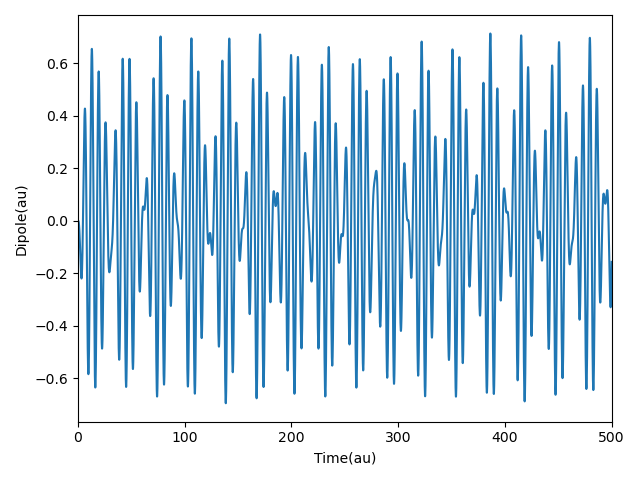
\includegraphics[width=\textwidth]{ch4/Figs/7-4.png}
     \end{subfigure}
     \caption{Rabi oscillation simulations of \ch{H_{2}} with external fields having intensities of 0.0445 au (left column) and 0.0890 au (right column). The first row displays results of $|A(t_{0}, t)|^{2}$ to indicate the population of the ground state at time $t$. The second row shows the corresponding induced dipole.}
     \label{fig:h2-rabi}
\end{figure}
%% C2H4-rabi
\subsubsubsection{\ch{C_{2}H_{4}}}\label{results-cc3-312}
With the existing formalism, \ch{C_{2}H_{4}} is also an interesting test case for Rabi oscillation. As a multi-electron molecule, it does not have the basic energy levels like \ch{H_{2}}. However, the $\pi$ and $\pi^{*}$ orbitals of the double bond can be approximately viewed as a two-level system. The calculation is conducted with the core orbitals frozen for efficiency. The number of active occupied orbitals and virtual orbitals is 6 each, using the STO-3G basis set. The frequency of the field is chosen to be 0.489 au (13.31 eV), which corresponds to the lowest excitation energy, corresponding to the $\pi$-$\pi^{*}$ transition as shown in the absorption spectrum in Fig.~\ref{fig:c2h4-abs}.
% Fig11: C2H4-abs
\begin{figure}
   \centering
   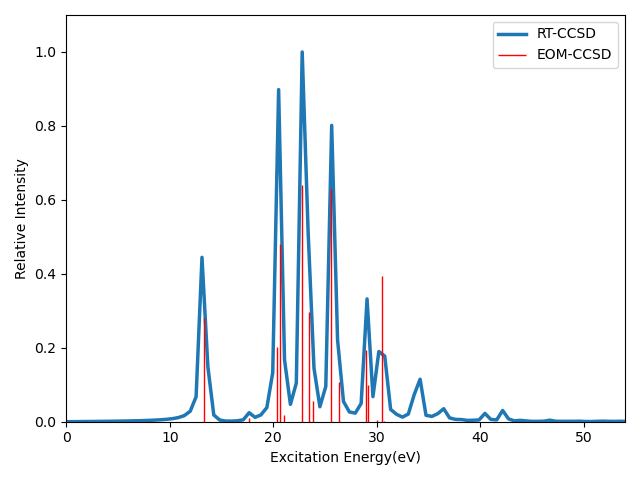
\includegraphics[angle=0, scale=0.43]{ch4/Figs/8-1.png}
   \caption{RT-CCSD/STO-3G linear absorption spectrum of \ch{C_{2}H_{4}} and corresponding EOM-CCSD/STO-3G transitions included as stick-spectra for comparison.}
     \label{fig:c2h4-abs}
\end{figure}

From the EOM-CCSD/STO-3G calculation, the leading contribution of this EOM state is the excitation from the highest occupied molecular orbital (HOMO) to the lowest unoccupied molecular orbital (LUMO), which corresponds to the specific $\hat{T}_{1}$ amplitude, $t_{5}^{0}$. Note that the orbital numbering starts from zero; thus, $t_{5}^{0}$ is associated with the sixth occupied orbital, the HOMO, and the first unoccupied orbital, the LUMO. If the state of the molecule at time $t$ can be expanded as a linear combination of all stationary point states, $t_{5}^{0}$ is the leading term of the coefficient of the lowest excited state. $|t_{5}^{0}|^{2}$ can thus be viewed as the population of this specific state. 

An additional autocorrelation function can be formulated using the ground state and a state vector with $t_{5}^{0}$ being the only nonzero amplitude at time $t$. Fig.~\ref{fig:c2h4-rabi} shows the population of the ground state on the left and the probability of the $\pi$-$\pi^{*}$ transition on the right. Unlike the success in simulating the Rabi oscillation of \ch{H_2}, the propagation is numerically unstable. From the figure on the left, the square of the autocorrelation function initially decreases from 1, reaches its minimum around 0.13, and then increases drastically, leading to a failure of the propagation.

In previous works on RT-CC methods, it has been demonstrated that the depletion of the ground state can cause a crash of the calculation. CC takes the ground state as the leading and reference state, while the ground state is no longer the most populated state due to the external field.\cite{Kristiansen2020} Although the value of the autocorrelation function does not diverge precisely at its minimum around 290 au, the population of the lowest excited state shown on the right confirms that $|t_{5}^{0}|^{2}$ diverges more rapidly as it moves beyond 0.5 and approaches one around 290 au. 

It is not clear why the simulation fails for the approximate Rabi oscillation of \ch{C_{2}H_{4}}, while it works for the Rabi oscillation of \ch{H_{2}}. Orbital-optimized methods may be good candidates for this situation, as they have been shown to work well for applying intense external fields when the population of the ground state approaches zero.\cite{Kristiansen2020} Such methods may also help identify the discrepancy between the approximate two-level system in the double bond and the exact two-level system. Further exploration is needed. 
% Fig10: C2H4-Rabi
\begin{figure}
     \centering
     \begin{subfigure}{0.45\textwidth}
         \centering
         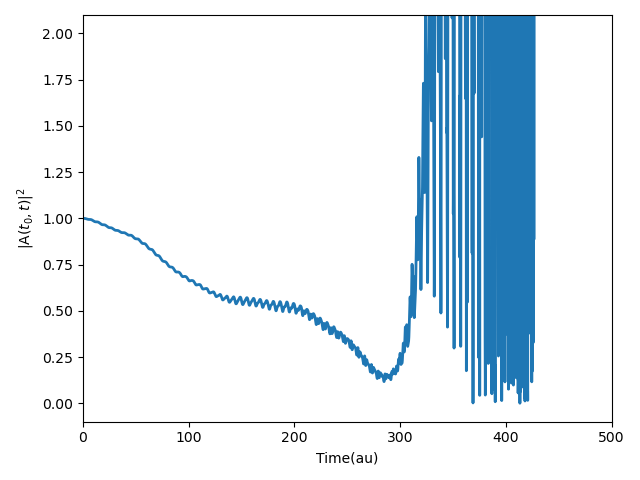
\includegraphics[width=\textwidth]{ch4/Figs/9-1.png}
     \end{subfigure}
     \hfill
     \begin{subfigure}{0.45\textwidth}
         \centering
         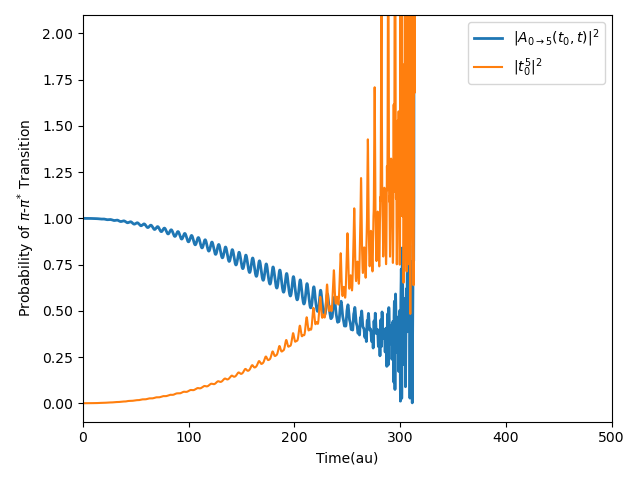
\includegraphics[width=\textwidth]{ch4/Figs/9-2.png}
      \end{subfigure}
     \caption{Rabi oscillation simulation of \ch{C_{2}H_{4}}. The intensity and frequency of the external field are chosen to be 0.01 au and 0.489 au, respectively. The left figure displays $|A(t_{0}, t)|^{2}$, indicating the population of the ground state at time $t$. The right one shows the probability of the targeted $\pi$-$\pi^{*}$ transition, represented by the square of the autocorrelation function and the square of $\hat{T}_{1}$ amplitude associated with the transition. The simulation lasts for 500 au, with the `cut off' of the curve indicating the time when the values diverge.}
     \label{fig:c2h4-rabi}
\end{figure}

\subsubsection{Population of the excited states}\label{results-cc3-32}
%%H2-ge
\subsubsubsection{\ch{H_{2}}}\label{results-cc3-321}
% Fig8: H2-Rabi-g-e
\begin{figure}
     \centering
     \begin{subfigure}{0.47\textwidth}
         \centering
         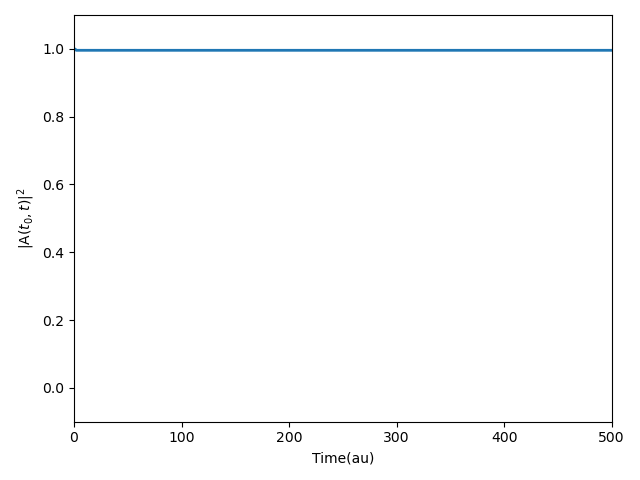
\includegraphics[width=\textwidth]{ch4/Figs/10-1.png}
     \end{subfigure}
     \hfill
     \begin{subfigure}{0.47\textwidth}
         \centering
         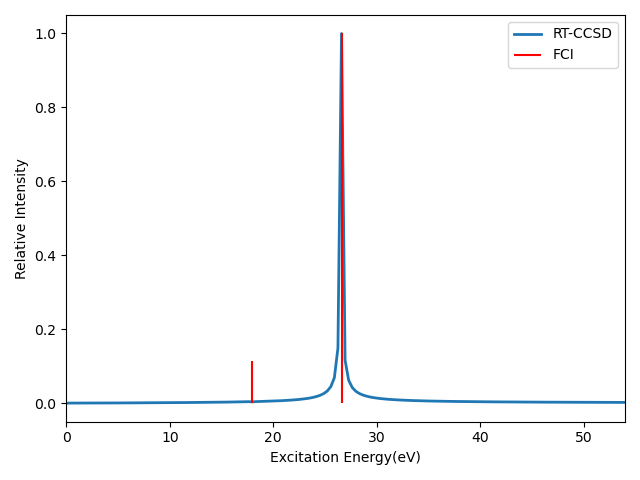
\includegraphics[width=\textwidth]{ch4/Figs/10-2.png}
      \end{subfigure}
       \vfill
     \begin{subfigure}{0.47\textwidth}
         \centering
         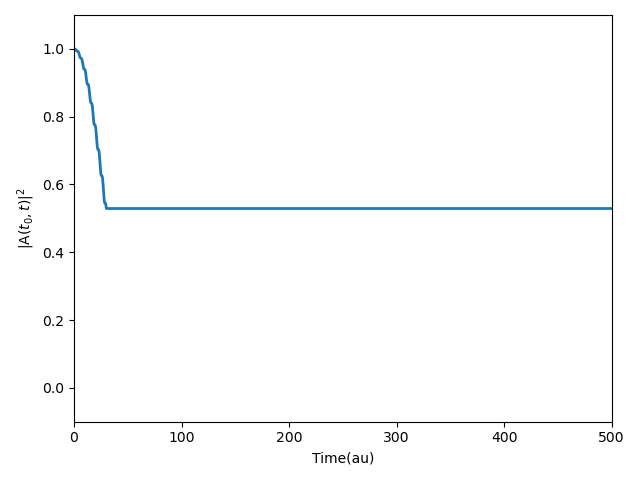
\includegraphics[width=\textwidth]{ch4/Figs/10-3.png}
     \end{subfigure}
     \hfill
     \begin{subfigure}{0.47\textwidth}
         \centering
         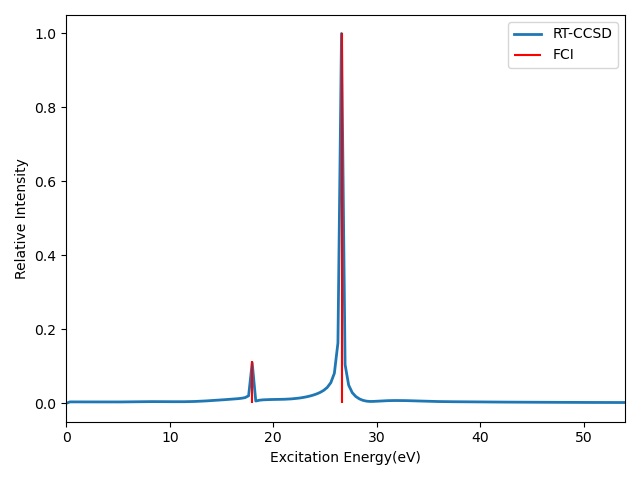
\includegraphics[width=\textwidth]{ch4/Figs/10-4.png}
     \end{subfigure}
      \vfill
     \begin{subfigure}{0.47\textwidth}
         \centering
         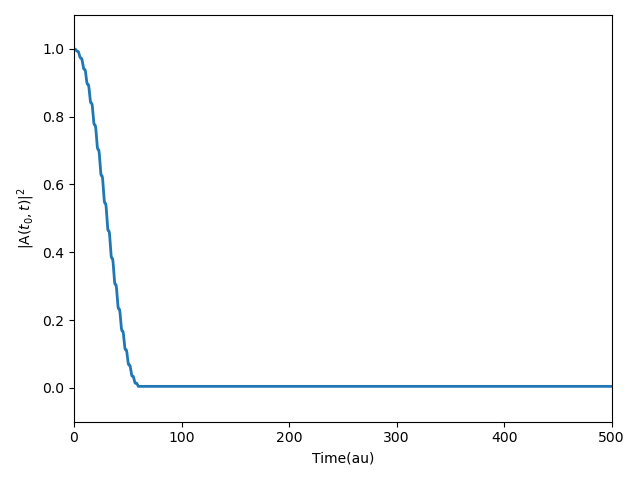
\includegraphics[width=\textwidth]{ch4/Figs/10-5.png}
     \end{subfigure}
     \hfill
     \begin{subfigure}{0.47\textwidth}
         \centering
         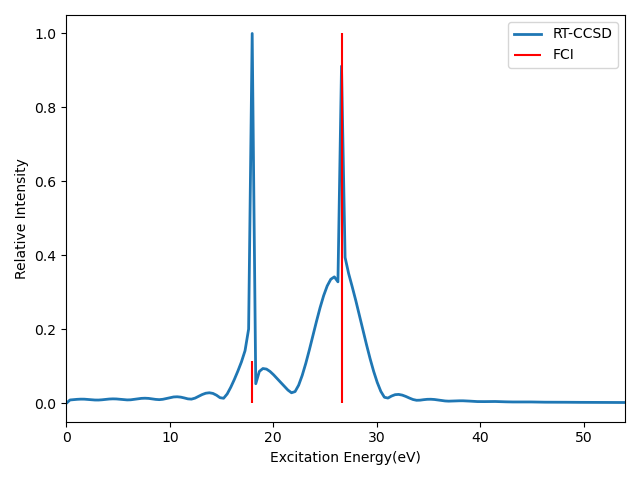
\includegraphics[width=\textwidth]{ch4/Figs/10-6.png}
     \end{subfigure}
     \caption{RT-CCSD/STO-3G results of \ch{H_{2}} with the external field applied for 2 au, 30 au, and 60 au. The left column displays the results of $|A(t_{0}, t)|^{2}$, indicating the population of the ground state at time $t$. The right column shows the corresponding absorption spectra. FCI/STO-3G transitions are included as stick spectra for comparison.}
     \label{fig:h2-ge}
\end{figure}
Besides the Rabi oscillation itself, details about the population of each state can provide additional information about the electron dynamics. To target different state populations in the RT propagation, the duration of the applied field can be varied according to the Rabi frequency obtained from the Rabi oscillation simulation. As shown in Fig.~\ref{fig:h2-ge}, the propagations are run for a total of 500 au. The field lasts for 2 au, 30 au, or 60 au, with the resulting $|A(t_{0}, t)|^{2}$ and absorption spectrum shown in the first, second, and third rows of Fig.~\ref{fig:h2-ge}, respectively.

When the field is turned off after only 2 au, $|A(t_{0}, t)|^{2}$ decreases slightly and remains close to 1 for the rest of the propagation. The resulting absorption spectrum reflects the singly-excited state correctly. When the duration of the field is increased to 30 au, $|A(t_{0}, t)|^{2}$ can be reduced to around 0.5, indicating a 50\% chance of finding the molecule in its ground state. A second peak appears in the lower frequency region of the spectrum. When the field is on for 60 au, the ground state is depleted, as shown by the decline of $|A(t_{0}, t)|^{2}$ from one to zero. As the duration of the field increases, the secondary peak becomes more prominent. The quality of the absorption spectrum is also diminished due to the deviation from the ground state.

In addition, the density matrix can be utilized to check the population of different states, as the diagonal elements represent the occupation numbers of the molecular orbitals. When the field is switched off after 2 au, the occupation number of the occupied orbital (OO) becomes 1.971, while the occupation number of the virtual orbital (OV) becomes 0.029, which is not far from the ground state. For the calculation where the field lasts for 30 au, NO$=1.496$ and NV$=0.504$. For the 60 au case, NO$=0.999$ and NV$=1.001$. The sum of NO and NV is the total number of electrons. These values are consistent with the corresponding autocorrelation functions. However, this does not explain the additional peak in the absorption spectra.

To identify the excited states, FCI results from Ref.~\citenum{Provorse2015} are included as stick spectra. In Ref.~\citenum{Provorse2015}, Provorse et al. discussed the population of the doubly-excited state S$_{2}$ from both TDCI and RT-TDDFT simulations of the Rabi oscillation, where RT-TDDFT has an artificial peak shift due to the limitation of the exchange functional. For our RT-CCSD calculation, the left and right peaks match the excitation energy from S$_{1}$ to S$_{2}$ and the excitation energy from S$_{0}$ to S$_{1}$, respectively. For an EOM-CCSD calculation with the RHF reference, only one transition from S$_{0}$ to S$_{1}$ can be obtained. The spectrum shows that the population of S$_{2}$ is not zero and increases with the decrease in ground state population induced by the applied field. The excitation energy can be obtained from the absorption spectrum, although the implementation is built upon an RHF formalism.
%% LiH-ge
\subsubsubsection{\ch{LiH}}\label{results-cc3-322}
To further explore the transitions to excited states caused by the external field, an oscillatory field is applied to \ch{LiH} for one optical cycle. The frequency is chosen to be the excitation energy associated with the $\sigma$-$\sigma^{*}$ transition, which is 0.652 au as obtained from the EOM-CCSD/STO-3G calculation. The duration of the field is therefore 9.64 au, while the total length of the propagation is 500 au. A reference absorption spectrum with a thin Gaussian pulse as the applied field is shown in Fig.~\ref{fig:lih-abs}, where the peaks match the EOM-CCSD results for the ground state to excited state transitions.

As shown in the left column of Fig.~\ref{fig:lih-ge}, the population of the ground state decreases with the increase in the field strength, resulting in a larger probability of ground state to excited state and excited state to excited state transitions. In the resulting absorption spectra on the right, in addition to the ground to excited state transitions, the excited to excited state transitions, labeled as thinner sticks for the reference value, are found and become more populated when the field strength is increased to 0.15 au. If the intensity is further increased to 0.45 au, some of the transitions become more obvious, but the stability of the propagation and the line shape of the spectrum are no longer ideal.

Overall, the RT-CCSD calculation can recover most of the excited state to excited state transitions, although they are still weaker than the ground state to excited state transitions. A reasonable field strength needs to be selected to ensure that the electrons can be excited while retaining the stability of the calculation.
% Fig9: LiH-abs
\begin{figure}
   \centering
   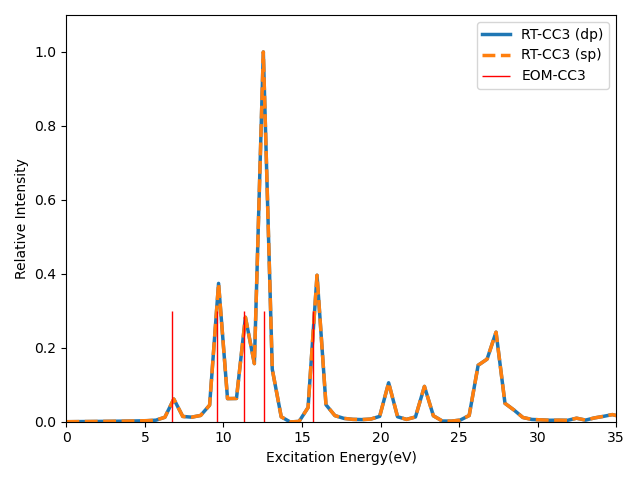
\includegraphics[angle=0, scale=0.43]{ch4/Figs/1-1.png}
   \caption{RT-CCSD/STO-3G linear absorption spectrum of \ch{LiH} and corresponding EOM-CCSD/STO-3G transitions included as stick-spectra for comparison.}
     \label{fig:lih-abs}
\end{figure}
% Fig10: LiH-g-e
\begin{figure}
     \centering
     \begin{subfigure}{0.47\textwidth}
         \centering
         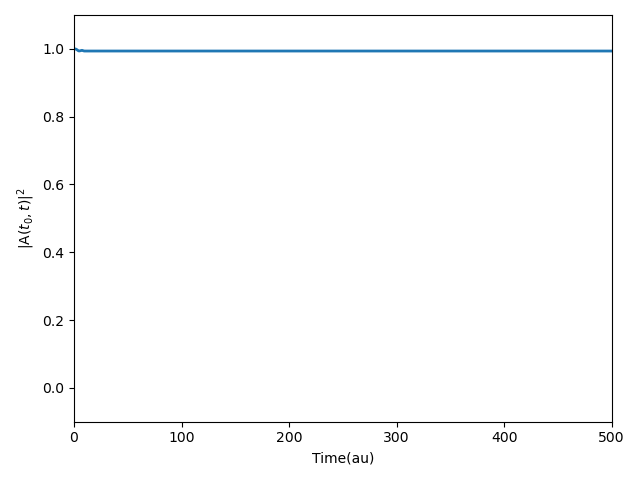
\includegraphics[width=\textwidth]{ch4/Figs/12-1.png}
     \end{subfigure}
     \hfill
     \begin{subfigure}{0.47\textwidth}
         \centering
         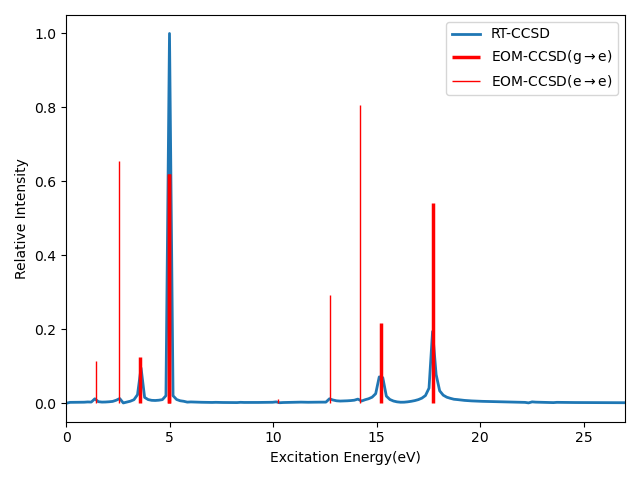
\includegraphics[width=\textwidth]{ch4/Figs/12-2.png}
      \end{subfigure}
       \vfill
     \begin{subfigure}{0.47\textwidth}
         \centering
         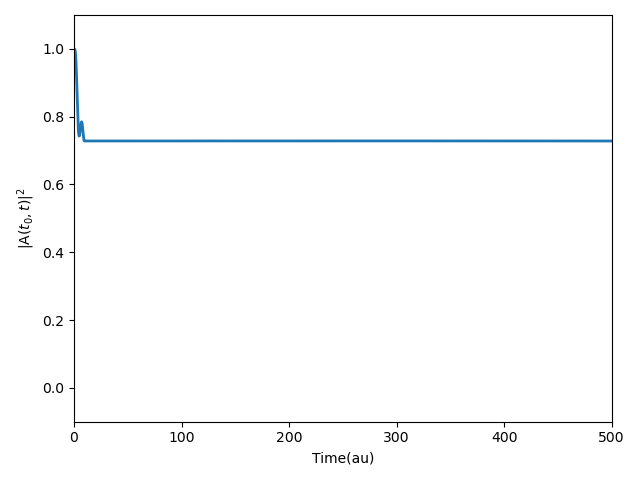
\includegraphics[width=\textwidth]{ch4/Figs/12-3.png}
     \end{subfigure}
     \hfill
     \begin{subfigure}{0.47\textwidth}
         \centering
         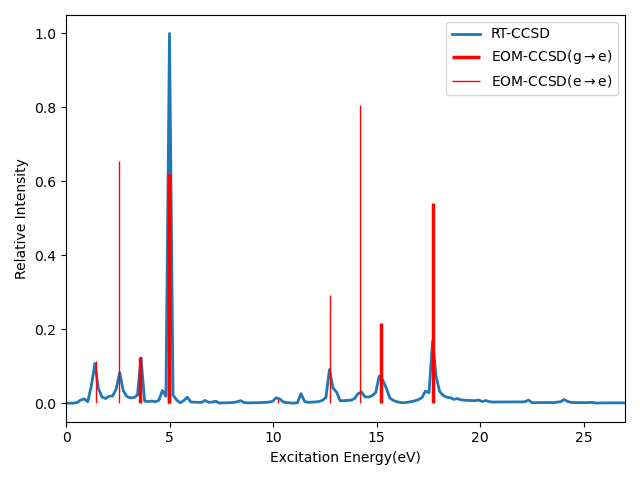
\includegraphics[width=\textwidth]{ch4/Figs/12-4.png}
     \end{subfigure}
      \vfill
     \begin{subfigure}{0.47\textwidth}
         \centering
         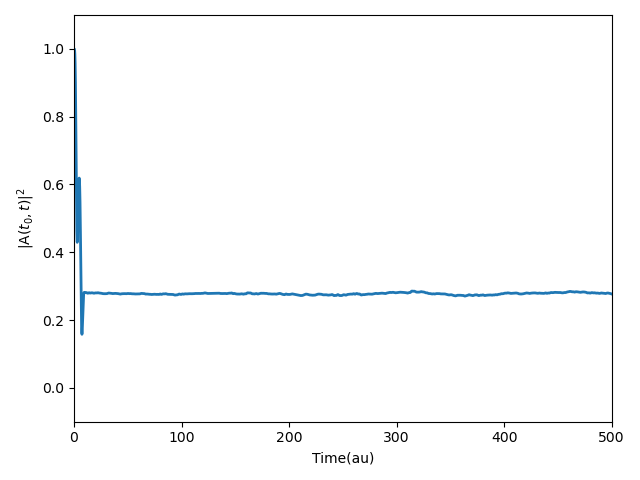
\includegraphics[width=\textwidth]{ch4/Figs/12-5.png}
     \end{subfigure}
     \hfill
     \begin{subfigure}{0.47\textwidth}
         \centering
         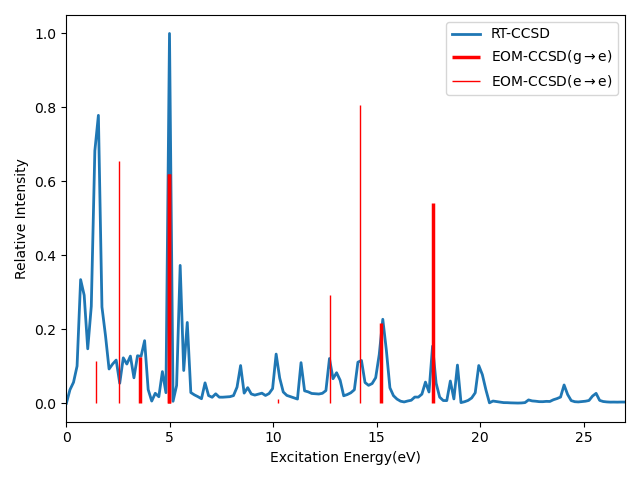
\includegraphics[width=\textwidth]{ch4/Figs/12-6.png}
     \end{subfigure}
     \caption{RT-CCSD/STO-3G results of \ch{LiH} with external fields of varying intensities (0.01 au, 0.15 au, and 0.45 au) applied for a duration of 500 au. The left column displays the evolution of the ground state population $|A(t_{0}, t)|^{2}$ over time $t$, while the right column showcases the corresponding absorption spectra. Stick-spectra of EOM-CCSD/STO-3G transitions are included for comparison.}
     \label{fig:lih-ge}
\end{figure}
\section{Conclusions}\label{conc_cc3}
The RT-CC3 method has been implemented with additional single-precision and GPU options. The working equations of RT-CC3 in the closed-shell and spin-adapted formalism are provided, with considerations of optimizing the performance in terms of reducing the number of higher-order tensor contractions. The implementation has been validated through the calculation of the absorption spectrum of \ch{H_{2}O} in both single- and double-precision. Numerical experiments have also been conducted with water clusters to test the computational cost of RT-CC3 simulations. It has been found that the use of GPUs can significantly speed up calculations by up to a factor of 17 due to the computational power they provide for tensor contractions. The acceleration gained from utilizing either GPUs or single-precision arithmetic needs to be observed significantly within a relatively large system (e.g., 72 molecular orbitals). To achieve the theoretical speedup, a much larger system is needed, however, optimization of memory allocation will also need to be taken into account because of the limited memory available on GPUs and the overhead of data migration. With the promising results of our Python implementation, exploring a productive-level code is worthwhile, especially for making the RT-CC3 method, which scales at $N^{7}$, feasible for large system/basis set and/or long RT propagations.  

For the calculation of optical properties, we have demonstrated that RT-CC3 is a feasible tool to obtain dynamic polariazabilities, first hyperpolarizabilities, and the $G'$ tensor with good agreement to LR-CC3 and a reasonable computational cost. The type of applied field, the precision arithmetic and the level of theory were tested with \ch{H_{2}O}. It has been proven through all test cases, including our new RT-CC3 method, that the QRCW can substantially improve curve fitting substantially and requires only two optical cycles for propagation. Especially for first hyperpolarizabilites, the curve of the second-order dipole moments from LRCW calculation has `discontinuities' in some places, leading to a large error and a low R$^{2}$ value for curve fitting. The QRCW is required here to obtain reliable results. The same is found in $G'$ tensor results, where some shifts appear in the curve of the induced magnetic dipole moments from LRCW calculations but not the QRCW ones. Regarding the single-precision calculations, no discrepancy is found in the polarizabilities and $G'$ tensor elements that are associated with the first derivative of electric and magnetic dipole moments, respectively. A significant difference, however, is found in the first hyperpolarizabilities. Although the QRCW can still reduce the error compared to the LRCW, single-precision results remain less accurate compared to double-precision results. These conclusions hold for both RT-CCSD and RT-CC3. 

Additionally, ten-electron systems including \ch{Ne}, \ch{HF}, \ch{H_{2}O}, \ch{NH_{3}} and \ch{CH_{4}} are used to test the calculation of polarizabilities with RT-CCSD, RT-CC3, and particularly TDNOCCD. It has been observed that the accuracy drops significantly when the frequency is closer to the resonance, while for the small frequencies, RT-CC3 matches LR-CC3 and FCI with errors less than 0.1\%. The trend of the error of RT-CC3 is consistent with RT-CCSD for most cases, except for the two values with the highest chosen frequencies of \ch{NH_{3}} and \ch{CH_{4}}. We have shown that the CC3 polarizabilities increases slightly faster when the frequency moves towards resonance, which may lead to a larger error. The TDNOCCD results show that the explicit orbital optimization lowers the polarizability values compared to RT-CCSD, where the only difference in these two methods is the orbital optimization. Compared to RT-CC3, TDNOCCD results are closer to LR-CC3/FCI results when RT-CC3 largely overestimates the results, otherwise, RT-CC3 yields more accurate results. 

Finally, the Rabi oscillation is simulated for \ch{H_{2}} and \ch{C_{2}H_{4}}. For \ch{H_{2}}, the Rabi oscillation between the ground state and the singly-excited state has been successfully reproduced. However, the simulation of the approximate two-level system, $\pi$-$\pi^{*}$ of the double bond, cannot be conducted. The propagation is no longer numerically stable, and the amplitudes diverge when the population of the ground state approaches zero. The reason why RT simulations act differently for the two systems is uncertain. Additional investigation is needed to locate the source of the problem. Using orbital-optimized methods may be a good starting point to determine if stability can be recovered. Using the same applied field but only keeping it on for a short amount of time at the beginning of the propagation, the transition to doubly-excited state of \ch{H_{2}} is observed from the absorption spectrum, although the RT-CC framework is built upon a RHF reference. Furthermore, the field is applied for one optical cycle for \ch{LiH}, with various field strengths. With the increasing field strength, the transitions can be found in the absorption spectrum, not only for ground state to ground state transitions, but also for excited state to excited state transitions. As stated earlier, although only RT-CCSD simulations were carried out for this section, RT-CC3 can be used in the same fashion if needed. 

    \chapter{Conclusions} \label{conc}
In this work, we have explored how molecules interact with external electromagnetic fields using real-time methods. The study began by establishing a framework that can be generally applied to RT-CC methods with varying levels of accuracy. Through this, we attempted a GPU implementation, single-precision calculations, and various numerical integration techniques to enhance the efficiency and numerical stability of the method. Additionally, we investigated the implementation of a higher level of theory, CC3, within the RT framework. A range of optical properties were calculated and then compared to results obtained from conventional linear response theory. Providing context and an overview of this topic, the background and objectives are summarized in Chapter 1. The relevant theoretical frameworks, including coupled cluster methods, response theory, and real-time methods, are presented in Chapter 2.

Chapter 3 focused on enhancing the computational efficiency of RT-CC methods in several aspects. Firstly, single-precision arithmetic was applied and tested for the calculation of the absorption spectrum of the water molecule, considering both computational speed and memory usage. Random noise of varying magnitudes was introduced to the double-precision results to assess the impact of precision level. No significant difference was observed between single- and double-precision absorption spectra in the water cluster test cases. The calculation was accelerated by a factor of 1.5 to 2 for a moderately larger system size.

Secondly, a GPU implementation was developed to accelerate tensor contractions, which represent the most resource-intensive part of the calculation. To minimize modifications to the existing CPU implementation, PyTorch was utilized to replace NumPy for tensor operations. The contractions were performed using {\tt opt\_einsum} with PyTorch backend. Numerical experiments demonstrated that the speedup from GPUs increases with system size. For the water tetramer test case, a speedup of a factor of 14 was achieved. This speedup is expected to continue growing for larger systems until it reaches the memory limit of GPUs.

Lastly, a family of Runge-Kutta integrators for the explicit propagation of wave function parameters in RT methods was studied and implemented. The explicit integrator was initially introduced and used to convey the fundamental concepts of numerical integration. Adaptive integrators, capable of adjusting the step size based on the local error at each time step, were further tested for potential speedup while maintaining numerical stability. Results showed that adaptive integrators can achieve a speedup compared to explicit integrators of the same order, assuming there are no abrupt changes in the trajectory.

For strong-field calculations, a mixed-step-size approach inspired by adaptive integrators was developed. This approach targets the rapidly increasing coupled cluster amplitudes when the field is active. A small step size, such as $10^{-5}$ au, is chosen for that period, while a larger step size, such 0.01 au, is used for the remainder of the propagation. This approach effectively stabilizes the calculation with minor overhead, especially when a thin Gaussian pulse is used as the external field.

In Chapter 4, we have formulated and implemented the RT-CC3 method to achieve a higher level of accuracy in comparison to the prevailing RT-CCSD method. Within the CC3 model, singles are designated as zeroth-order in perturbation theory and treated as parameters for orbital relaxation. Triples are computed in each iteration, with updated singles and doubles, and are employed to calculate their contributions to the new amplitude residuals.

The RT-CC3 absorption spectrum of the water molecule was computed in both single- and double-precision. It was demonstrated that these two levels of precision yield identical spectra that align with the EOM-CC3 results. Furthermore, the performance of both GPU and CPU implementations was evaluated using the same water cluster test cases introduced in Chapter 3. The results clearly indicated that the runtime of RT-CC3 calculations was notably longer than that of RT-CCSD, due to the $N^{7}$ scaling. However, through the utilization of GPUs, a significant speedup of up to a factor of 17 was achieved.

Beyond the absorption spectrum, RT-CC3 has been extended to compute higher-order properties and to be compared against other RT methods. Dynamic optical properties, encompassing polarizabilities, first hyperpolarizabilities, and the $G'$ tensor, were obtained using the finite difference method to calculate the first and second-order derivatives of the time-dependent induced electric and magnetic dipole moments. In comparison to their double-precision counterparts, single-precision calculations were also conducted.

From the numerical tests on the water molecule, it was observed that the quadratic ramped continuous wave (QRCW), which ensures an adiabatic switch-on, yielded more accurate results and higher curve fitting quality compared to the linear ramped continuous wave (LRCW). Concerning polarizabilities, the single- and double-precision results were identical and differed from the linear response (LR) results by less than 0.1\%. For first hyperpolarizabilities, a discrepancy between single- and double-precision arithmetic was observed, with single-precision results being less accurate. The results showed larger errors, up to 2.56\% for single-precision and 0.93\% for double-precision, which stemmed from the higher-order dipole moments compared to polarizabilities. Results of the $G'$ tensor were similar to polarizabilities, exhibiting no significant difference between single- and double-precision results and maintaining a high-quality curve fitting.

Furthermore, RT-CCSD and RT-CC3 polarizabilities were compared to time-dependent nonorthogonal orbital-optimized coupled cluster doubles (TDNOCCD) results for five ten-electron systems. It was demonstrated that the accuracy of RT results decreased as the corresponding frequencies approached resonance. The orbital optimization within TDNOCCD led to smaller polarizability values across various systems and frequencies, in comparison to RT-CCSD and RT-CC3.

With our RT implementation, we have also conducted simulations involving electron dynamics, including Rabi oscillations and transitions to excited states. The Rabi oscillation of the hydrogen molecule was successfully reproduced by applying an oscillatory field with the excitation energy from the ground state to the singly-excited state as the frequency. The population of the ground state, represented by the square of the autocorrelation function of the ground state and the state vector at each time step, fluctuated between 0 and 1. The frequency, position of the wave crest, and trough matched the characteristics of a general Rabi oscillation.

A similar simulation was attempted for the Rabi oscillation of an approximate two-level system, $\pi$-$\pi^{*}$ of \ch{C_{2}H_{4}}. However, the propagation encountered issues around the time when the ground state was depleted. While this behavior might be reasonable considering our RT methods are built upon a single reference, the distinct difference compared to the simulation of \ch{H_{2}} remains unexplained with the current results.

In addition to the Rabi oscillation, we observed transitions between excited states for the \ch{H_{2}} and \ch{LiH} test cases, particularly when the frequency of the external field was selected to match the $\sigma$-$\sigma^{*}$ transition. As the field strength increased, a corresponding enhancement in the relative intensities of the excited state to excited state transitions was demonstrated in the absorption spectra.

Overall, this work has demonstrated the process of obtaining optical properties using RT-CC methods and enhancing the efficiency of these calculations. Through the development of the RT-CC framework, the established infrastructure, GPU implementation, and distinct precision arithmetics are readily applicable to various levels of theory with minimal adjustments. Simulations have confirmed that our RT-CC implementation offers a functional and user-friendly tool for computing frequency-dependent optical properties in the time domain.

For future investigations, the potential development of a production-level code incorporating the GPU implementation could expand the capacity to compute optical properties for larger systems. Additionally, collaborative efforts with experimental scientists are anticipated, as the parameters of the external field can be tailored to match experimental setups within the existing RT framework.

    %%%% ADDING TO TRY TO FIX BIB....
    \bibliographystyle{achemso}

      
	% This is the standard bibtex file. Do not include the .bib extension in <bib_file_name>.
	% Uncomment the following lines to include your bibliography: 
	\bibliography{refs,ch3/refs_ch3}
	%\bibliographystyle{plainnat}   

	% This formats the chapter name to appendix to properly define the headers:
	\appendix
	% Add your appendices here. You must leave the appendices enclosed in the appendices environment in order for the table of contents to be correct.
%	\begin{appendices}
%% TODO: SI for Ch4: geometries
%		\chapter{Supporting Information for Basis Set Superposition Errors in the Many-Body Expansion of Molecular Properties} \label{si:mbe}
 %      \input{p1/si.tex}
 %     \end{appendices}
	
\end{document}


%****************************************************************************
% Below are some general suggestions for writing your dissertation:
%
% 1. Label everything with a meaningful prefix so that you
%    can refer back to sections, tables, figures, equations, etc.
%    Usage \label{<prefix>:<label_name>} where some suggested
%    prefixes are:
%			ch: Chapter
%     		se: Section
%     		ss: Subsection
%     		sss: Sub-subsection
%			app: Appendix
%     		ase: Appendix section
%     		tab: Tables
%     		fig: Figures
%     		sfig: Sub-figures
%     		eq: Equations
%
% 2. The VTthesis class provides for natbib citations. You should upload
%	 one or more *.bib bibtex files. Suppose you have two bib files: some_refs.bib and 
%    other_refs.bib.  Then your bibliography line to include them
%    will be:
%      \bibliography{some_refs, other_refs}
%    where multiple files are separated by commas. In the body of 
%    your work, you can cite your references using natbib citations.
%    Examples:
%      Citation                     Output
%      -------------------------------------------------------
%      \cite{doe_title_2016}        [18]
%      \citet{doe_title_2016}       Doe et al. [18]
%      \citet*{doe_title_2016}      Doe, Jones, and Smith [18]
%
%    For a complete list of options, see
%      https://www.ctan.org/pkg/natbib?lang=en
%
% 3. Here is a sample table. Notice that the caption is centered at the top. Also
%    notice that we use booktabs formatting. You should not use vertical lines
%    in your tables.
% 
%				\begin{table}[htb]
%					\centering
%					\caption{Approximate computation times in hh:mm:ss for full order 						versus reduced order models.}
%					\begin{tabular}{ccc}
%						\toprule
%						& \multicolumn{2}{c}{Computation Time}\\
%						\cmidrule(r){2-3}
%						$\overline{U}_{in}$ m/s & Full Model & ROM \\
%						\midrule
%						0.90 & 2:00:00 & 2:08:00\\
%						0.88 & 2:00:00 & 0:00:03\\
%						0.92 & 2:00:00 & 0:00:03\\
%						\midrule
%						Total & 6:00:00 & 2:08:06\\
%						\bottomrule
%					\end{tabular}
%					\label{tab:time_rom}
%				\end{table}
% 
% 4. Below are some sample figures. Notice the caption is centered below the
%    figure.
%    a. Single centered figure:
%					\begin{figure}[htb]
%						\centering
%						\includegraphics[scale=0.5]{my_figure.eps}
%						\caption{Average outlet velocity magnitude given an average  
%				        input velocity magnitude of 0.88 m/s.} 
%						\label{fig:output_rom}
%					\end{figure}
%    b. Two by two grid of figures with subcaptions
%					\begin{figure}[htb]
%						\centering
%						\begin{subfigure}[h]{0.45\textwidth}
%							\centering
%							\includegraphics[scale=0.4]{figure_1_1.eps}
%							\caption{Subcaption number one}
%							\label{sfig:first_subfig}
%						\end{subfigure}
%						\begin{subfigure}[h]{0.45\textwidth}
%							\centering
%							\includegraphics[scale=0.4]{figure_1_2.png}
%							\caption{Subcaption number two}
%							\label{sfig:second_subfig}
%						\end{subfigure}
%
%						\begin{subfigure}[h]{0.45\textwidth}
%							\centering
%							\includegraphics[scale=0.4]{figure_2_1.pdf}
%							\caption{Subcaption number three}
%							\label{sfig:third_subfig}
%						\end{subfigure}
%						\begin{subfigure}[h]{0.45\textwidth}
%							\centering
%							\includegraphics[scale=0.4]{figure_2_2.eps}
%							\caption{Subcaption number four}
%							\label{sfig:fourth_subfig}
%						\end{subfigure}
%						\caption{Here is my main caption describing the relationship between the 4 subimages}
%						\label{fig:main_figure}
%					\end{figure}
%
%----------------------------------------------------------------------------
%
% The following is a list of definitions and packages provided by VTthesis:
%
% A. The following packages are provided by the VTthesis class:
%      amsmath, amsthm, amssymb, enumerate, natbib, hyperref, graphicx, 
%      tikz (with shapes and arrows libraries), caption, subcaption,
%      listings, verbatim
%
% B. The following theorem environments are defined by VTthesis:
%      theorem, proposition, lemma, corollary, conjecture
% 
% C. The following definition environments are defined by VTthesis:
%      definition, example, remark, algorithm
%
%----------------------------------------------------------------------------
%
%  I hope this template file and the VTthesis class will keep you from having 
%  to worry about the formatting and allow you to focus on the actual writing.
%  Good luck, and happy writing.
%    Alan Lattimer, VT, 2016
%
%****************************************************************************





